\documentclass[conference]{IEEEtran}
\IEEEoverridecommandlockouts
\usepackage{cite}
\usepackage{amsmath,amssymb,amsfonts}
\usepackage{algorithmic}
\usepackage{graphicx}
\usepackage{textcomp}
\usepackage{xcolor}
\usepackage{hyperref}
\usepackage{float}

\def\BibTeX{{\rm B\kern-.05em{\sc i\kern-.025em b}\kern-.08em
    T\kern-.1667em\lower.7ex\hbox{E}\kern-.125emX}}
\begin{document}

\title{Clasificación de Dígitos en Audio MNIST usando LeNet-5 y Técnicas de Preprocesamiento}

\author{
    \IEEEauthorblockN{Tomás Granados}
    \IEEEauthorblockA{
        \textit{Escuela de Ingeniería en Computación} \\
        \textit{Instituto Tecnológico de Costa Rica} \\
        Cartago, Costa Rica \\
        Carné: 2021579524 \\
        \texttt{tomasgrapre@estudiantec.cr}
    }
    \and
    \IEEEauthorblockN{Daniel Garbanzo}
    \IEEEauthorblockA{
        \textit{Escuela de Ingeniería en Computación} \\
        \textit{Instituto Tecnológico de Costa Rica} \\
        San José, Costa Rica \\
        Carné: 2022117129 \\
        \texttt{dgarbanzo@estudiantec.cr}
    }
    \and
    \IEEEauthorblockN{José Pablo Granados}
    \IEEEauthorblockA{
        \textit{Escuela de Ingeniería en Computación} \\
        \textit{Instituto Tecnológico de Costa Rica} \\
        Cartago, Costa Rica \\
        Carné: 2022028503 \\
        \texttt{j.granados@estudiantec.cr}
    }
}

\maketitle

\begin{abstract}
En este trabajo se explora la clasificación de dígitos hablados utilizando el dataset Audio MNIST. Se implementan y comparan diferentes técnicas de preprocesamiento y modelos, enfocándose en el ajuste de hiperparámetros y el análisis de resultados sobre cuatro variantes del dataset. Se presentan los resultados obtenidos y se discute el impacto de cada técnica en el desempeño del clasificador.
\end{abstract}

\begin{IEEEkeywords}
Audio MNIST, LeNet-5, clasificación de audio, frequency masking, bilateral filter, ajuste de hiperparámetros, deep learning
\end{IEEEkeywords}

\section{Introducción}
El reconocimiento automático de voz es un área de investigación activa con aplicaciones en asistentes virtuales, accesibilidad y sistemas de control por voz. El objetivo de este trabajo es crear un clasificador para el dataset Audio MNIST~\cite{audio_mnist_original}, un benchmark ampliamente utilizado en la literatura para tareas de clasificación de audio y experimentación con arquitecturas de deep learning~\cite{audio_mnist_cnn,audio_mnist_transfer}. 

Se utilizaron cuatro variantes del dataset, aplicando técnicas como \textit{frequency masking}~\cite{audio_augmentation} y \textit{bilateral filter}, y se implementó el modelo LeNet-5~\cite{lenet5_original} como base para la clasificación, así como una arquitectura ResNet personalizada~\cite{resnet_original}. El ajuste de hiperparámetros se realizó de manera específica para cada variante del dataset, evaluando métricas como \textit{accuracy}, \textit{loss}, \textit{precision}, \textit{recall} y \textit{f1-score}.

La estructura del documento es la siguiente: en la Sección II se describe el dataset y las variantes utilizadas; en la Sección III se presenta el Modelo A (LeNet-5) y el análisis de sus resultados; en la Sección IV se presenta el Modelo B; finalmente, en la Sección V se realiza una comparación entre ambos modelos.



\section{Datasets}
Se utilizó el dataset de Audio MNIST \cite{audio_mnist_kaggle}, el cual consiste en grabaciones de audio de dígitos hablados por diferentes personas. Para este experimento, el dataset se dividió en cuatro variantes principales:

\begin{itemize}
    \item \textbf{Raw without data augmentation}
    \item \textbf{Raw with data augmentation}
    \item \textbf{Bilateral Filter without data augmentation}
    \item \textbf{Bilateral Filter with data augmentation}
\end{itemize}

La técnica de \textit{data augmentation} utilizada fue \textit{Frequency Masking} \cite{freq_masking_torch}, seleccionada debido a la corta duración de los audios (menos de 2 segundos). Se aplicó un máximo de 7 bins para evitar la pérdida excesiva de información.

Ejemplos visuales de las diferentes técnicas de preprocesamiento se muestran en la Figura~\ref{fig:masking} (\textit{frequency masking}), Figura~\ref{fig:bilateral} (\textit{bilateral filter}) y Figura~\ref{fig:raw} (sin preprocesamiento).

\begin{figure}[H]
\centerline{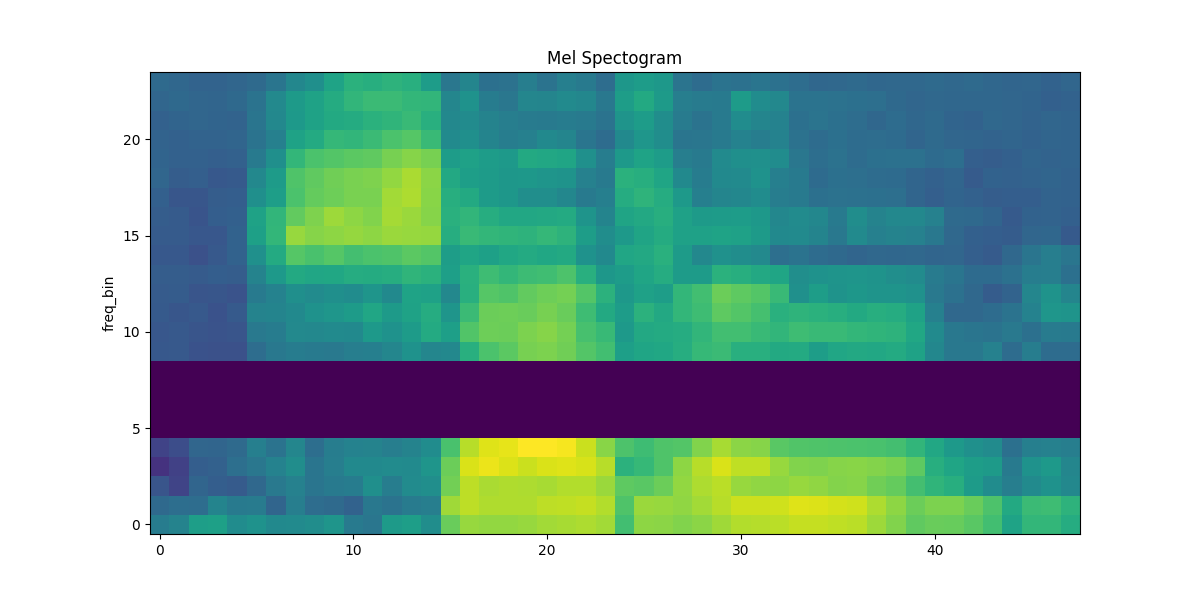
\includegraphics[width=0.45\textwidth]{sample_masking.png}}
\caption{Ejemplo de frequency masking aplicado a un espectrograma.}
\label{fig:masking}
\end{figure}
\noindent\textit{
La Figura~\ref{fig:masking} muestra un espectrograma al que se le ha aplicado la técnica de frequency masking. Se observa una franja horizontal oscura que representa la eliminación de ciertas bandas de frecuencia, lo cual simula la pérdida de información en el dominio frecuencial. Esta técnica de data augmentation ayuda a que el modelo sea más robusto ante variaciones y ruidos en las frecuencias, promoviendo una mejor generalización y reduciendo el riesgo de sobreajuste.
}

\begin{figure}[H]
\centerline{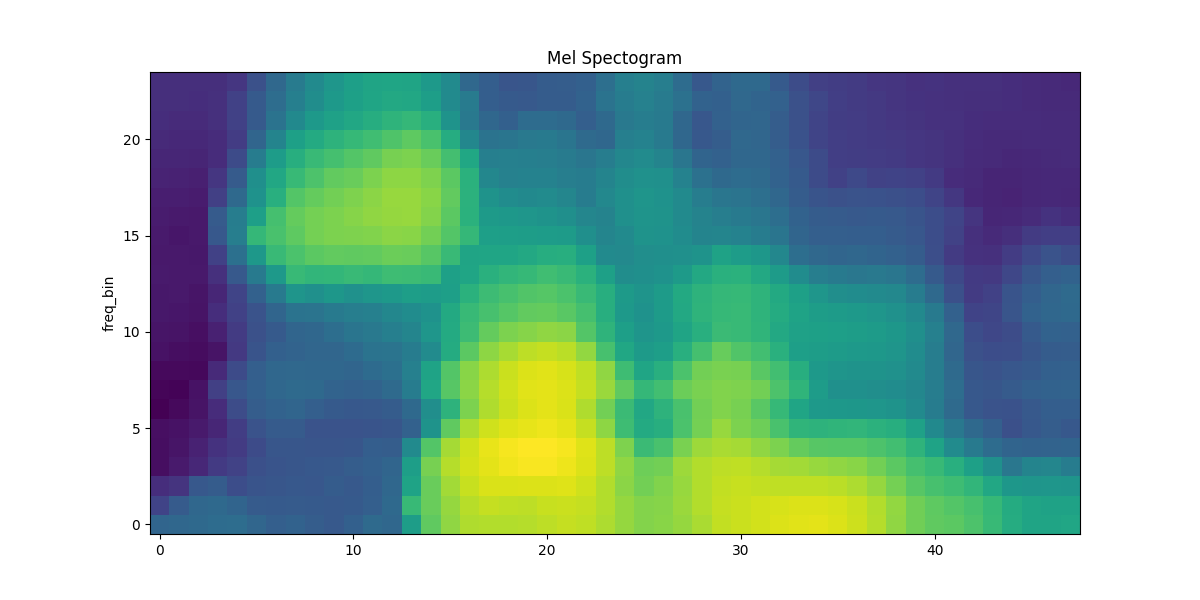
\includegraphics[width=0.45\textwidth]{sample_bilateral.png}}
\caption{Ejemplo de bilateral filter aplicado a un espectrograma.}
\label{fig:bilateral}
\end{figure}
\noindent\textit{
En la Figura~\ref{fig:bilateral} se presenta un espectrograma procesado con un filtro bilateral. Este filtro suaviza la imagen preservando los bordes, lo que resulta en una representación más nítida de las regiones de energía en el espectrograma. El uso de bilateral filter puede ayudar a resaltar patrones relevantes y reducir el ruido, facilitando que el modelo de aprendizaje profundo identifique características discriminativas en los datos de audio.
}

\begin{figure}[H]
\centerline{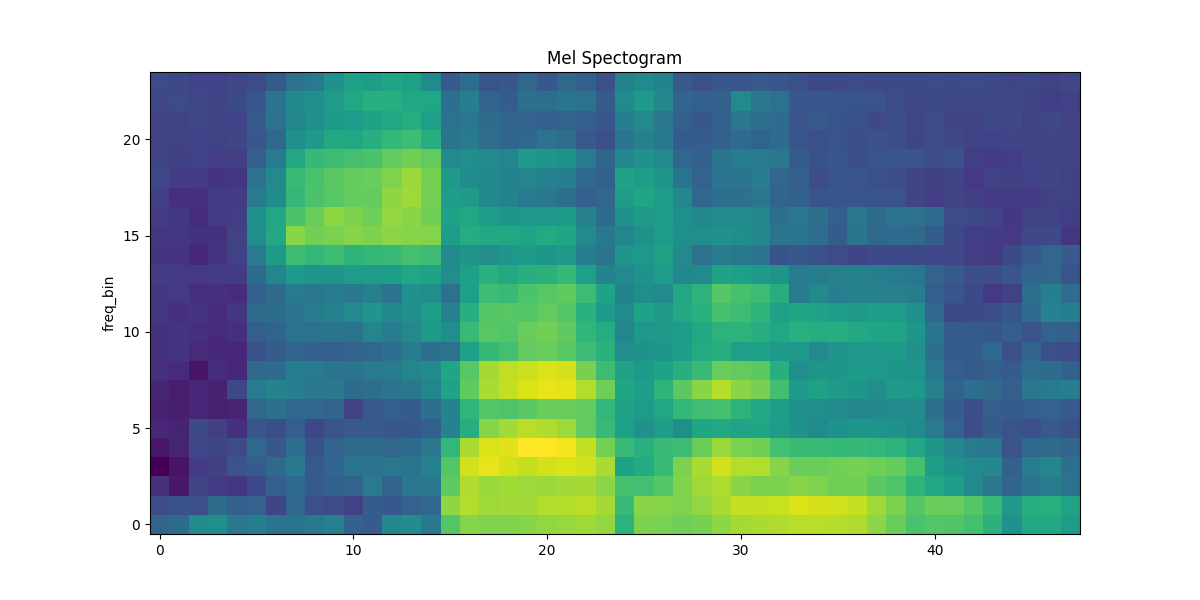
\includegraphics[width=0.45\textwidth]{sample.png}}
\caption{Ejemplo de espectrograma sin preprocesamiento.}
\label{fig:raw}
\end{figure}
\noindent\textit{
La Figura~\ref{fig:raw} muestra un espectrograma original, sin ningún tipo de preprocesamiento. Se pueden observar las variaciones de energía a lo largo del tiempo y las diferentes bandas de frecuencia. Este tipo de representación es la base para comparar el impacto de las técnicas de preprocesamiento, como frequency masking y bilateral filter, en el desempeño del modelo de clasificación.
}

\section{Modelo A: LeNet-5}

El modelo LeNet-5~\cite{lenet5_original} fue implementado tomando como referencia el notebook de Kaggle~\cite{lenet5_kaggle}. Se realizaron múltiples corridas para ajustar los hiperparámetros de acuerdo con el comportamiento de cada variante del dataset.

LeNet-5 es una arquitectura pionera en el campo de las redes neuronales convolucionales, originalmente propuesta para el reconocimiento de dígitos manuscritos, y ha sido adaptada exitosamente a tareas de clasificación de audio~\cite{audio_mnist_cnn}. Su simplicidad y eficiencia la convierten en un baseline robusto para comparar con arquitecturas más complejas en el dominio de audio~\cite{audio_cnn_review}.

La implementación consiste en una secuencia de capas convolucionales y de pooling, seguidas de capas lineales totalmente conectadas. En particular, se emplea una entrada de un solo canal (\texttt{n\_channels=1}), ya que los espectrogramas generados a partir de los audios son representaciones en escala de grises, es decir, matrices bidimensionales con un solo canal de información. 

El número de clases de salida (\texttt{n\_classes=10}) corresponde a los diez dígitos posibles (del 0 al 9) presentes en el dataset Audio MNIST, lo que permite que el modelo realice una clasificación multiclase adecuada para el problema planteado. La arquitectura mantiene la estructura original de LeNet-5, con dos bloques de convolución y pooling, seguidos de tres capas lineales, lo que proporciona un balance entre capacidad de representación y eficiencia computacional.

\subsection{Ajuste de Hiperparámetros}
El ajuste de hiperparámetros se realizó de manera independiente para cada variante del dataset. Para el modelo LeNet-5, se utilizó como línea base un \textit{learning rate} de 0.0001 y 15 \textit{epochs}.

\subsubsection{Raw with Data Augmentation}
Se realizaron 8 corridas con los siguientes hiperparámetros (ver Tabla~\ref{tab:raw_aug_hparams}).

\begin{table}[H]
\caption{Hiperparámetros de las corridas (Raw with Data Augmentation)}
\centering
\begin{tabular}{|c|c|c|}
\hline
\textbf{Corrida} & \textbf{Learning Rate} & \textbf{Epochs} \\
\hline
1 & 0.0001 & 15 \\
2 & 0.0001 & 30 \\
3 & 0.0010 & 15 \\
4 & 0.0005 & 15 \\
5 & 0.0005 & 20 \\
6 & 0.0007 & 20 \\
7 & 0.0007 & 25 \\
8 & 0.0007 & 30 \\
\hline
\end{tabular}
\label{tab:raw_aug_hparams}
\end{table}

Los resultados de cada corrida se pueden observar en la Tabla~\ref{tab:raw_aug_results} del Apéndice~\ref{appendix:results}.

\noindent\textit{
Al analizar la Tabla~\ref{tab:raw_aug_results}, se observa una mejora progresiva en las métricas de accuracy, F1-score, precisión y recall a medida que se ajustan los hiperparámetros, especialmente aumentando el número de épocas y el learning rate. La última corrida (corrida 8) presenta los mejores resultados en la mayoría de las métricas tanto para los conjuntos de prueba, entrenamiento y validación. Esto sugiere que el modelo se beneficia de un mayor número de épocas y un learning rate de 0.0007, permitiendo una mejor convergencia y generalización. Además, la pérdida (loss) es la más baja en esta corrida, lo que indica un ajuste óptimo del modelo sin señales de sobreajuste.
}

\subsection{Gráficas de Raw with Data Augmentation}

A continuación se presentan las gráficas de las métricas obtenidas para el dataset \textit{Raw with Data Augmentation}. Las primeras gráficas muestran la evolución de las métricas en los conjuntos de entrenamiento y validación, seguidas de las métricas por clase en el conjunto de prueba. Finalmente, se presenta la matriz de confusión obtenida.

% --- TRAIN/VAL ---

\begin{figure}[H]
    \centering
    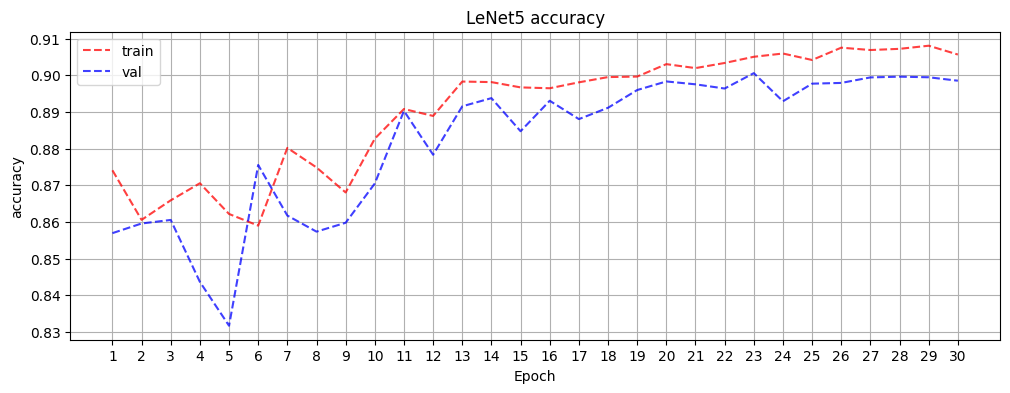
\includegraphics[width=0.95\linewidth]{graphics-raw-da/raw-da-accuracy-train_val.png}
    \caption{Accuracy en los conjuntos de entrenamiento y validación a lo largo de las épocas.}
    \label{fig:raw-da-accuracy-train_val}
\end{figure}
\noindent\textit{
La Figura~\ref{fig:raw-da-accuracy-train_val} muestra la evolución del accuracy durante el entrenamiento. Se observa una tendencia ascendente tanto en el conjunto de entrenamiento como en el de validación, alcanzando valores cercanos a 0.91 y 0.90 respectivamente. La cercanía entre ambas curvas indica que el modelo no está sobreajustando y que la generalización es adecuada. Esto valida la elección de los hiperparámetros y sugiere que el modelo está bien ajustado para este dataset.
}

\begin{figure}[H]
    \centering
    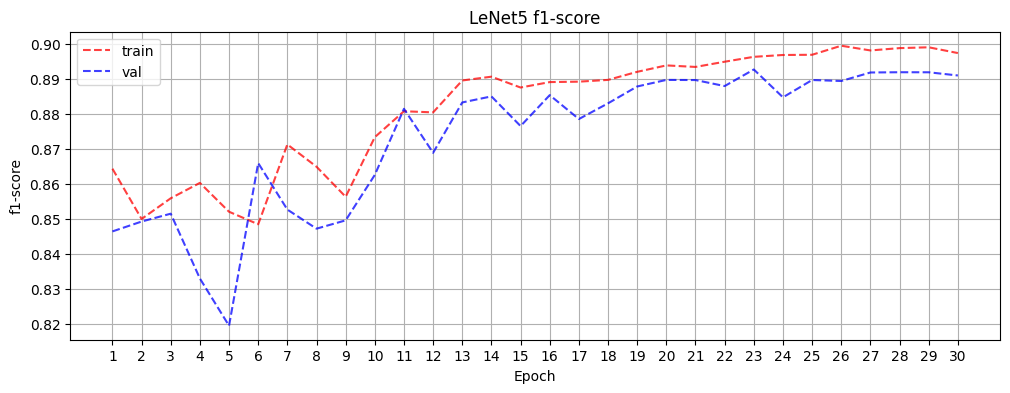
\includegraphics[width=0.95\linewidth]{graphics-raw-da/raw-da-f1score-train_val.png}
    \caption{F1-score en los conjuntos de entrenamiento y validación a lo largo de las épocas.}
    \label{fig:raw-da-f1score-train_val}
\end{figure}
\noindent\textit{
La Figura~\ref{fig:raw-da-f1score-train_val} muestra la evolución del F1-score durante el entrenamiento. Se observa una mejora progresiva y una convergencia entre los valores de entrenamiento y validación, lo que indica que el modelo mantiene un buen equilibrio entre precisión y recall a lo largo de las épocas. Esto respalda la estabilidad del modelo y la idoneidad de los hiperparámetros seleccionados.
}

\begin{figure}[H]
    \centering
    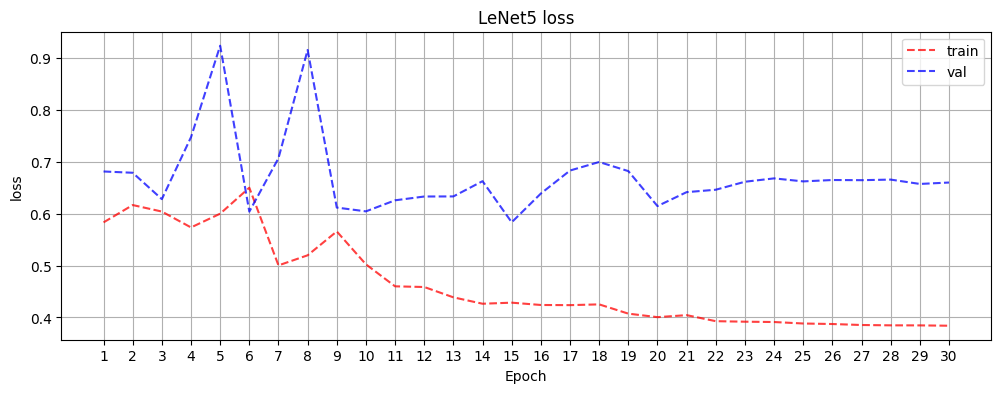
\includegraphics[width=0.95\linewidth]{graphics-raw-da/raw-da-loss-train_val.png}
    \caption{Loss en los conjuntos de entrenamiento y validación a lo largo de las épocas.}
    \label{fig:raw-da-loss-train_val}
\end{figure}
\noindent\textit{
En la Figura~\ref{fig:raw-da-loss-train_val} se observa la evolución de la función de pérdida (loss) para entrenamiento y validación. Aunque hay algunas fluctuaciones en las primeras épocas, ambas curvas tienden a estabilizarse, con la de entrenamiento alcanzando valores más bajos. La diferencia entre ambas curvas no es excesiva, lo que indica que el modelo no está sobreajustando y que la capacidad de generalización es adecuada.
}

\begin{figure}[H]
    \centering
    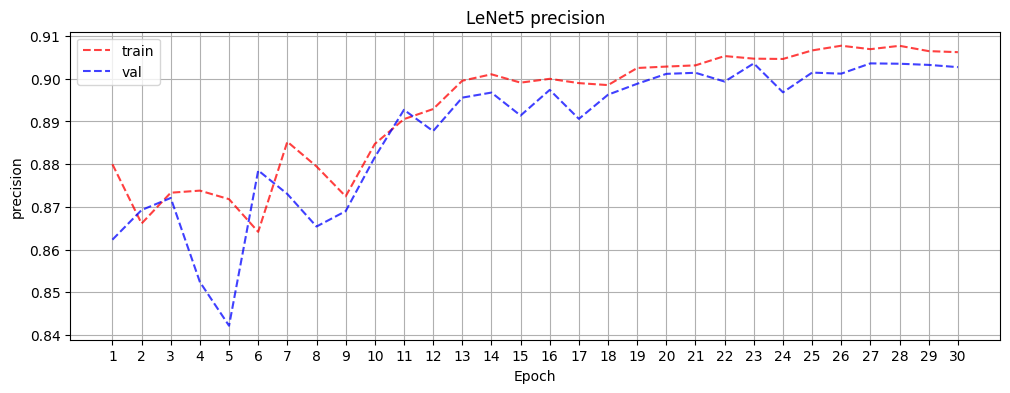
\includegraphics[width=0.95\linewidth]{graphics-raw-da/raw-da-precision-train_val.png}
    \caption{Precisión en los conjuntos de entrenamiento y validación a lo largo de las épocas.}
    \label{fig:raw-da-precision-train_val}
\end{figure}
\noindent\textit{
En la Figura~\ref{fig:raw-da-precision-train_val} se observa que la precisión aumenta de manera constante durante el entrenamiento, con valores finales cercanos a 0.91 para ambos conjuntos. La similitud entre ambas curvas indica que el modelo no está sobreajustando y que la precisión es consistente tanto en entrenamiento como en validación.
}

\begin{figure}[H]
    \centering
    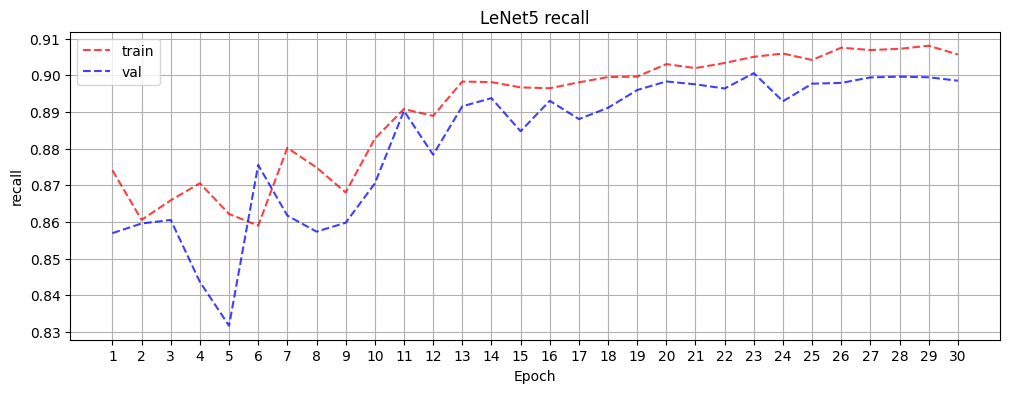
\includegraphics[width=0.95\linewidth]{graphics-raw-da/raw-da-recall-train_val.png}
    \caption{Recall en los conjuntos de entrenamiento y validación a lo largo de las épocas.}
    \label{fig:raw-da-recall-train_val}
\end{figure}
\noindent\textit{
Finalmente, la Figura~\ref{fig:raw-da-recall-train_val} muestra la evolución del recall durante el entrenamiento. Ambas curvas presentan una tendencia ascendente y convergente, alcanzando valores cercanos a 0.91. Esto indica que el modelo es capaz de identificar correctamente la mayoría de las instancias en ambos conjuntos, validando la robustez del entrenamiento y la selección de hiperparámetros.
}

% --- TEST ---

\begin{figure}[H]
    \centering
    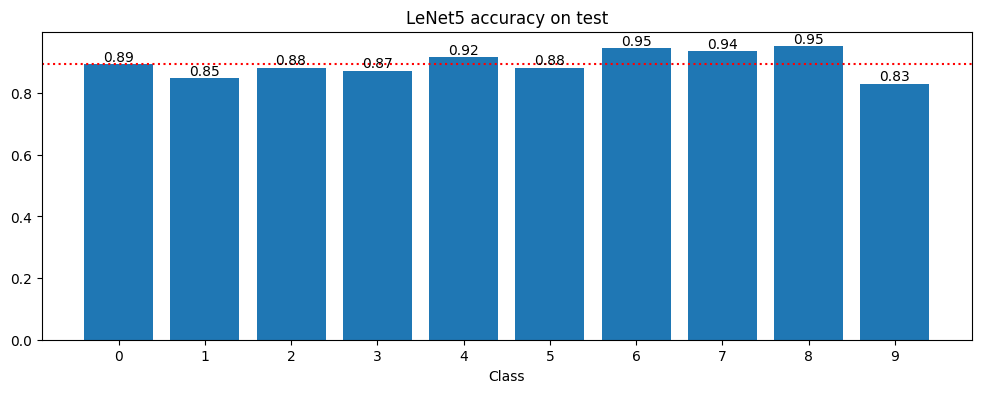
\includegraphics[width=0.95\linewidth]{graphics-raw-da/raw-da-accuracy-test.png}
    \caption{Accuracy por clase en el conjunto de prueba.}
    \label{fig:raw-da-accuracy-test}
\end{figure}
\noindent\textit{
En la Figura~\ref{fig:raw-da-accuracy-test} se observa que la precisión del modelo LeNet5 varía entre las diferentes clases, alcanzando valores superiores al 0.9 en las clases 4, 6, 7 y 8, mientras que la clase 9 presenta el menor desempeño (0.83). La línea roja punteada indica el promedio general de accuracy. Este análisis sugiere que el modelo tiene dificultades particulares con ciertas clases.
}

\begin{figure}[H]
    \centering
    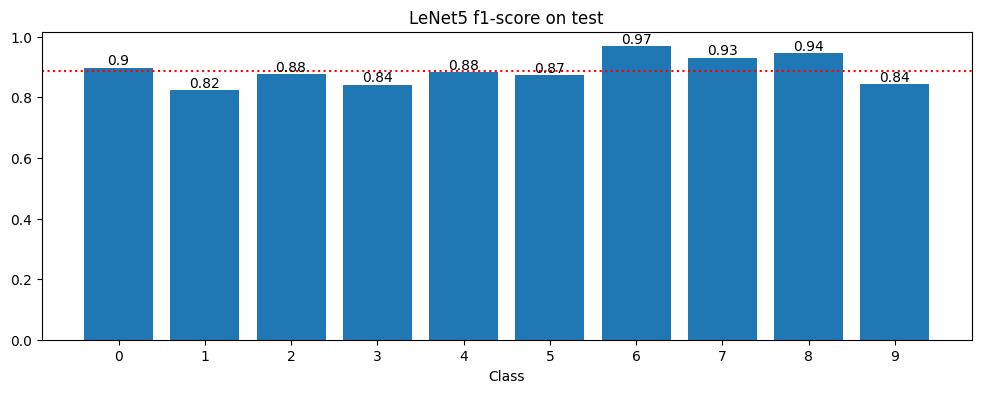
\includegraphics[width=0.95\linewidth]{graphics-raw-da/raw-da-f1score-test.png}
    \caption{F1-score por clase en el conjunto de prueba.}
    \label{fig:raw-da-f1score-test}
\end{figure}
\noindent\textit{
En la Figura~\ref{fig:raw-da-f1score-test} se aprecia el F1-score por clase. Al igual que con el accuracy, las clases 6, 7 y 8 presentan los mejores resultados, mientras que la clase 1 y la clase 9 muestran los valores más bajos. El F1-score promedio está representado por la línea roja punteada.
}

\begin{figure}[H]
    \centering
    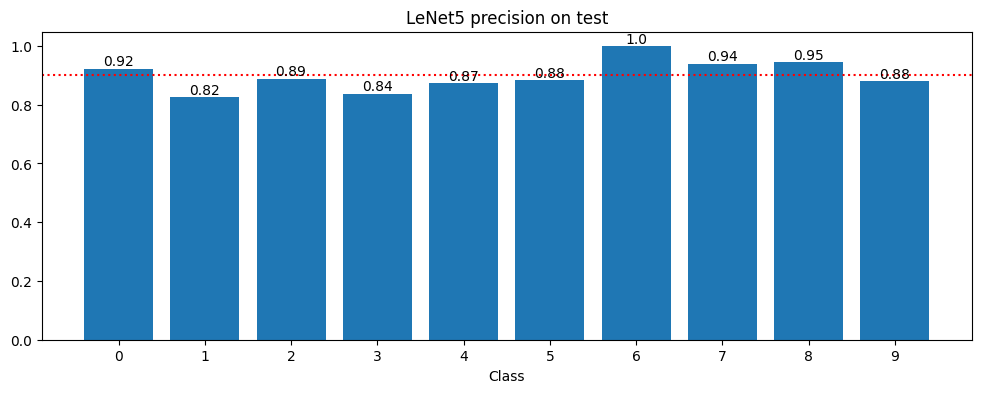
\includegraphics[width=0.95\linewidth]{graphics-raw-da/raw-da-precision-test.png}
    \caption{Precisión por clase en el conjunto de prueba.}
    \label{fig:raw-da-precision-test}
\end{figure}
\noindent\textit{
La Figura~\ref{fig:raw-da-precision-test} muestra la precisión por clase. Destaca la clase 6 con un valor perfecto de 1.0, mientras que las clases 1 y 3 presentan los valores más bajos (0.82 y 0.84 respectivamente). El promedio general está indicado por la línea roja punteada. Estos resultados sugieren que el modelo es especialmente confiable para ciertas clases.
}

\begin{figure}[H]
    \centering
    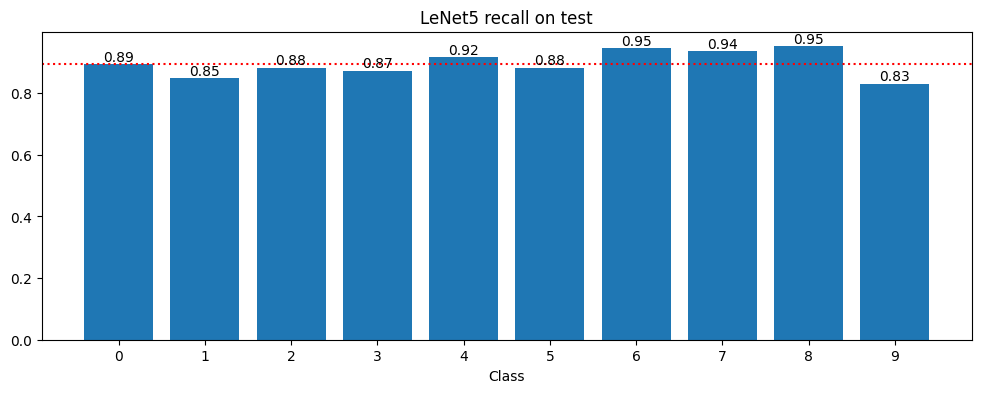
\includegraphics[width=0.95\linewidth]{graphics-raw-da/raw-da-recall-test.png}
    \caption{Recall por clase en el conjunto de prueba.}
    \label{fig:raw-da-recall-test}
\end{figure}
\noindent\textit{
La Figura~\ref{fig:raw-da-recall-test} muestra el recall por clase. Se observa un comportamiento similar al accuracy y F1-score, con las clases 6, 7 y 8 destacando, y la clase 9 mostrando el menor recall. Esto indica que el modelo tiene dificultades para identificar correctamente todas las instancias de la clase 9.
}

% --- MATRIZ CONFUSIÓN ---

\begin{figure}[H]
    \centering
    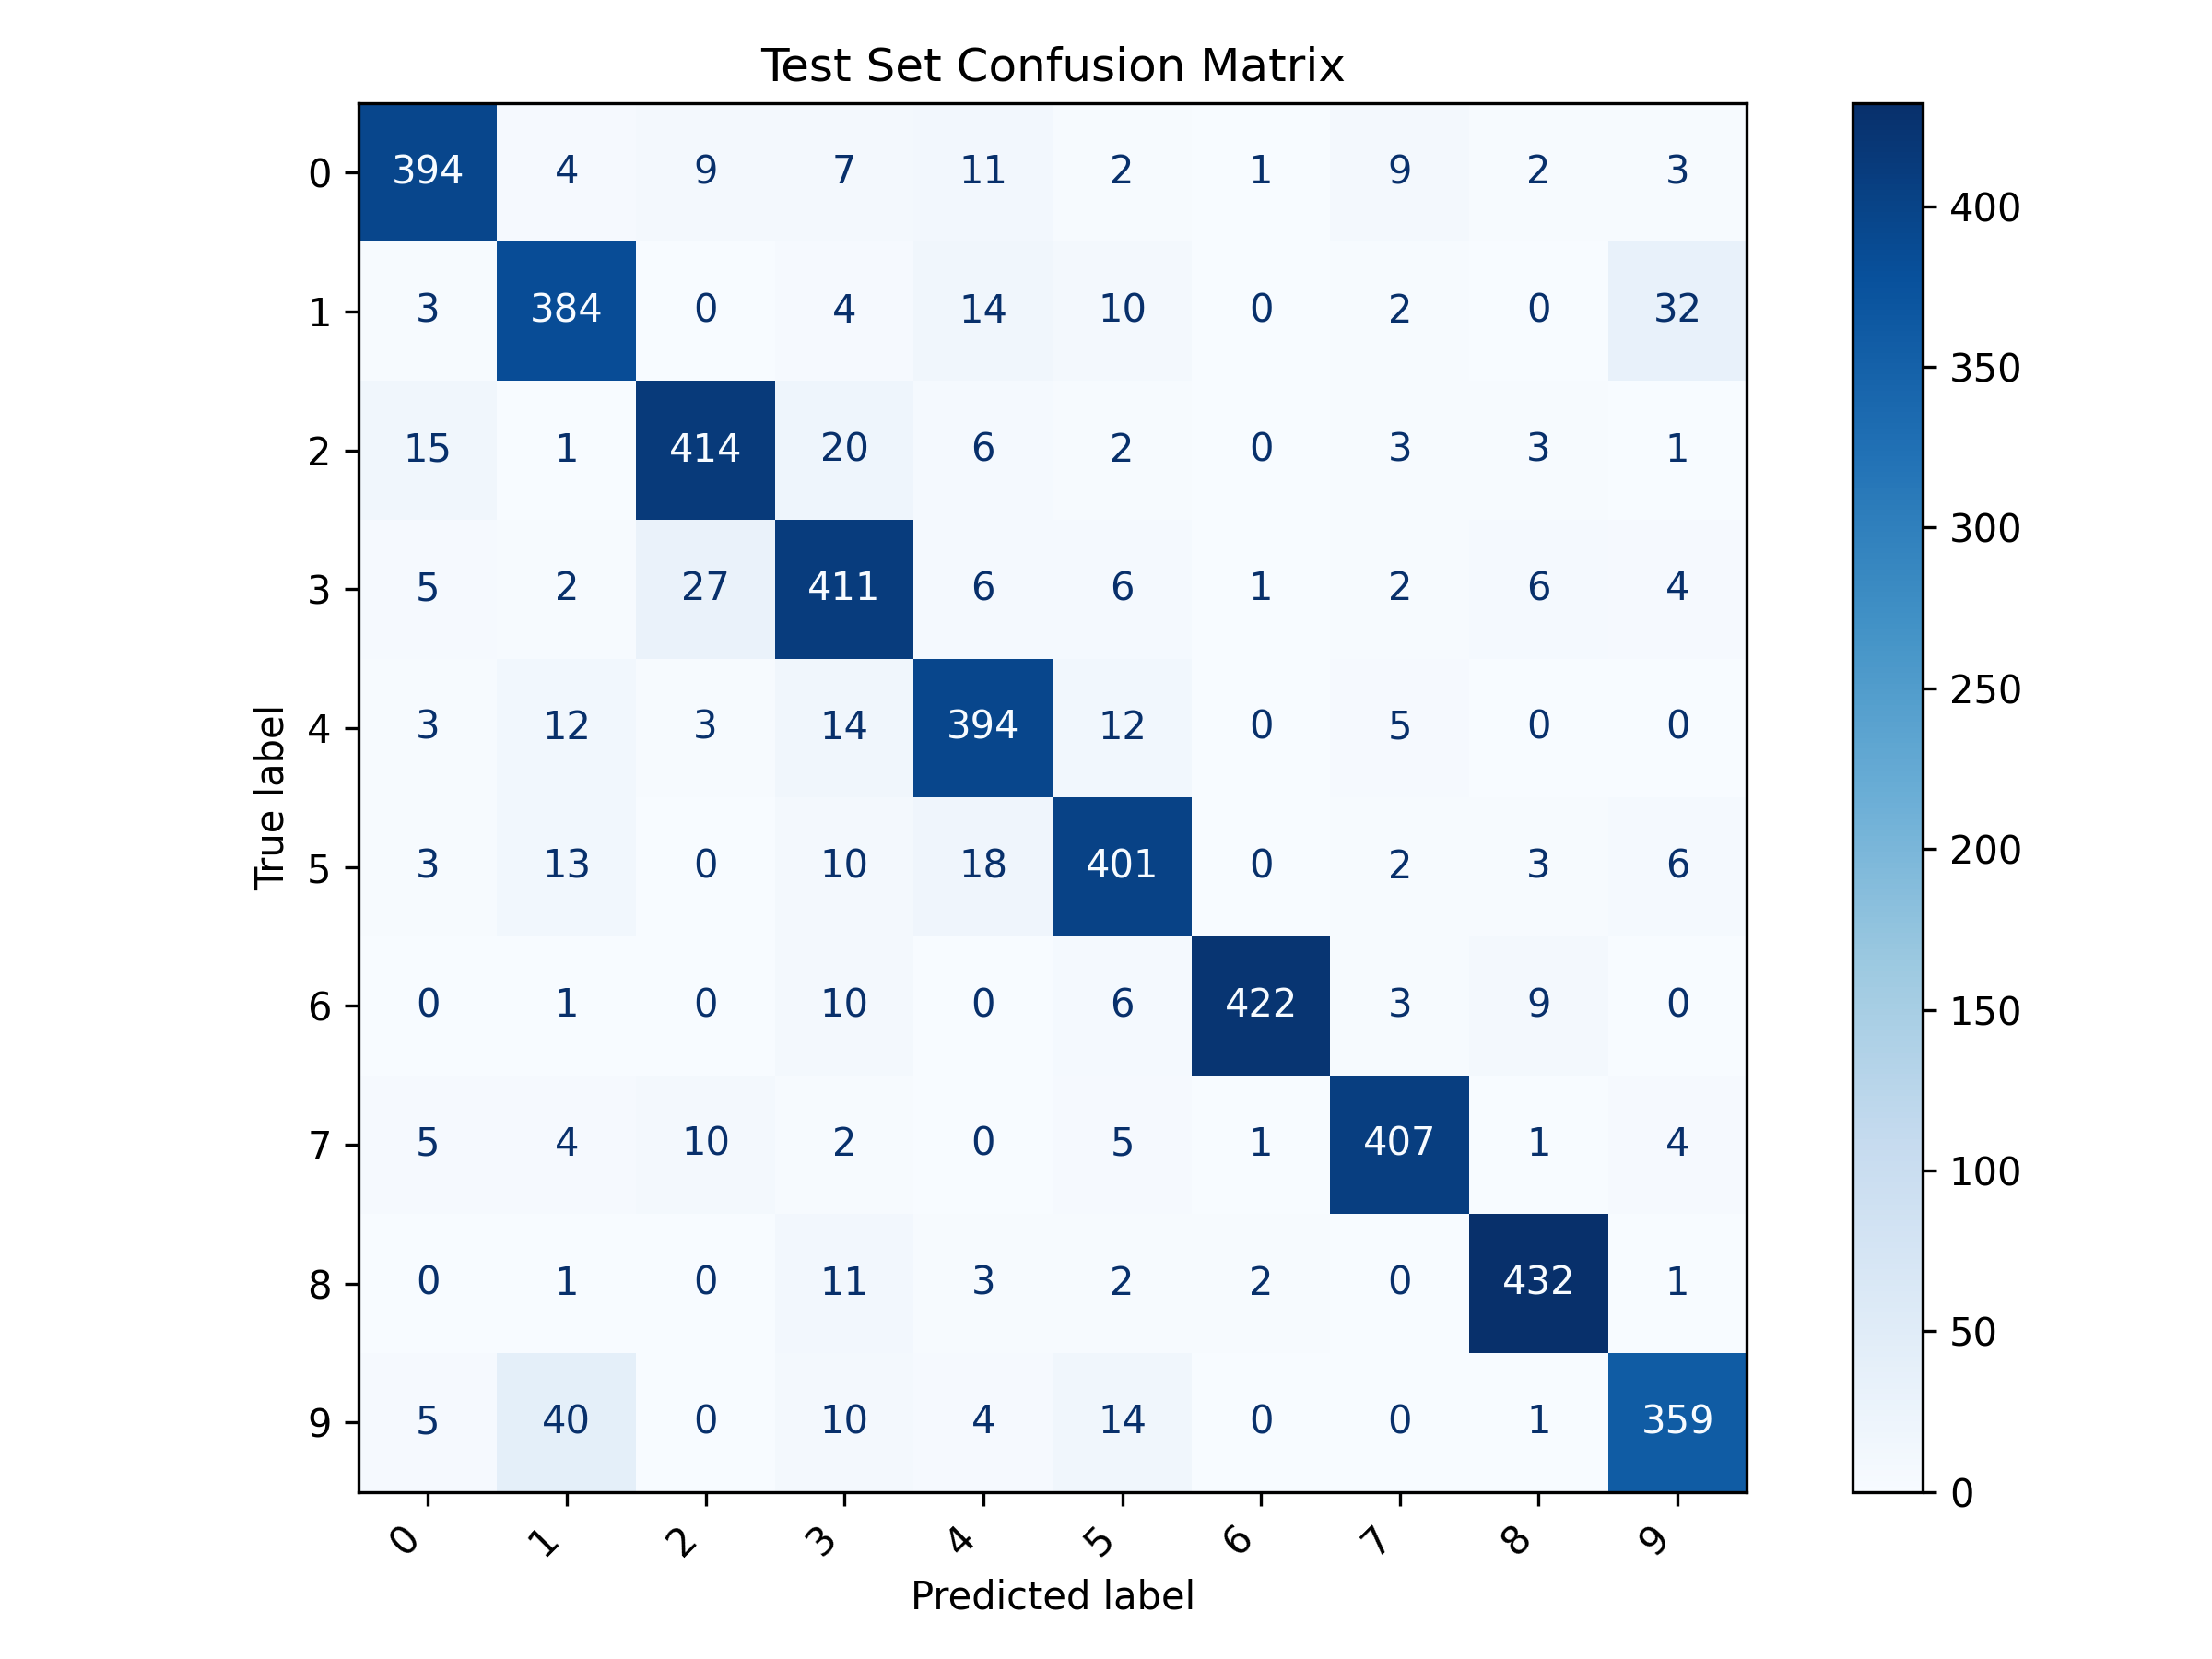
\includegraphics[width=0.95\linewidth]{graphics-raw-da/raw-da-confusion-matrix.png}
    \caption{Matriz de confusión del conjunto de prueba para Raw with Data Augmentation.}
    \label{fig:raw-da-confusion-matrix}
\end{figure}
\noindent\textit{
La Figura~\ref{fig:raw-da-confusion-matrix} muestra la matriz de confusión obtenida en el conjunto de prueba. Se observa que la mayoría de las predicciones se concentran en la diagonal principal, lo que indica un buen desempeño general del modelo. Sin embargo, existen confusiones notables entre algunas clases, especialmente la clase 9, que es confundida con la clase 1 en 40 ocasiones, y la clase 3, que es confundida con la clase 2 en 27 ocasiones. Estas confusiones sugieren que existen similitudes acústicas entre ciertos dígitos o posibles desbalances en el dataset.
}

\subsubsection{Raw without Data Augmentation}
Se realizaron 4 corridas con los siguientes hiperparámetros (ver Tabla~\ref{tab:raw_noaug_hparams}).

\begin{table}[H]
\caption{Hiperparámetros de las corridas (Raw without Data Augmentation)}
\centering
\begin{tabular}{|c|c|c|}
\hline
\textbf{Corrida} & \textbf{Learning Rate} & \textbf{Epochs} \\
\hline
1 & 0.0001 & 15 \\
2 & 0.0007 & 20 \\
3 & 0.0007 & 25 \\
4 & 0.0007 & 30 \\
\hline
\end{tabular}
\label{tab:raw_noaug_hparams}
\end{table}

Los resultados de cada corrida se pueden observar en la Tabla~\ref{tab:raw_noaug_results} del Apéndice~\ref{appendix:results}.

\noindent\textit{
En la Tabla~\ref{tab:raw_noaug_results} se aprecia una clara tendencia de mejora en las métricas a medida que se incrementan las épocas y se ajusta el learning rate. La última corrida (corrida 4) destaca por alcanzar los valores más altos de accuracy, F1-score, precisión y recall en todos los conjuntos, así como la menor pérdida (loss). Esto indica que el modelo logra un excelente ajuste y generalización bajo estas condiciones, beneficiándose de un mayor tiempo de entrenamiento y un learning rate de 0.0007.
}

\subsection{Gráficas de Raw without Data Augmentation}

A continuación se presentan las gráficas de las métricas obtenidas para el dataset \textit{Raw without Data Augmentation}. Se muestran primero las métricas de entrenamiento y validación, seguidas de las métricas por clase en el conjunto de prueba y, finalmente, la matriz de confusión.

% --- TRAIN/VAL ---

\begin{figure}[H]
    \centering
    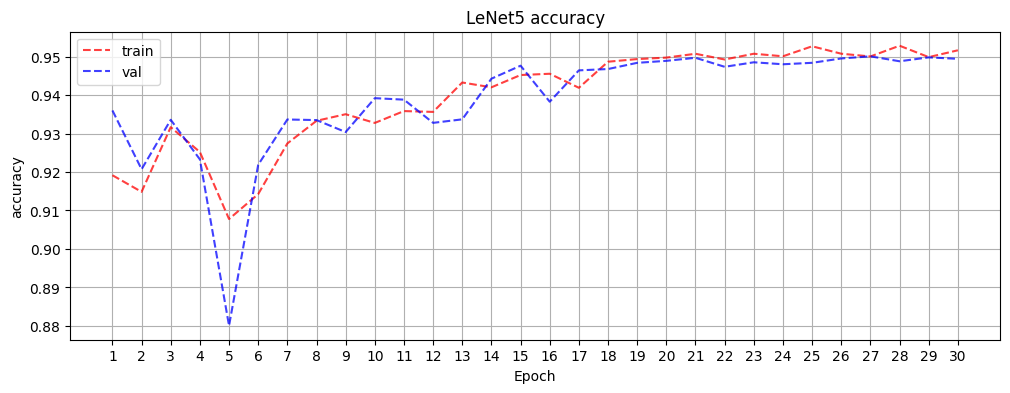
\includegraphics[width=0.95\linewidth]{graphics-raw/raw-accuracy-train_val.png}
    \caption{Accuracy en los conjuntos de entrenamiento y validación a lo largo de las épocas.}
    \label{fig:raw-accuracy-train_val}
\end{figure}
\noindent\textit{
La Figura~\ref{fig:raw-accuracy-train_val} muestra la evolución del accuracy durante el entrenamiento. Se observa una tendencia ascendente y una convergencia entre las curvas de entrenamiento y validación, alcanzando valores superiores a 0.95. Esto indica que el modelo logra un excelente desempeño y generalización, sin señales de sobreajuste.
}

\begin{figure}[H]
    \centering
    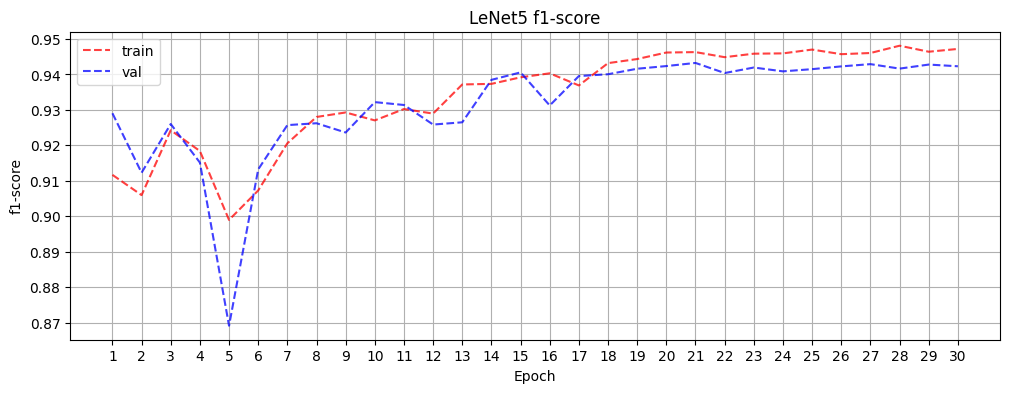
\includegraphics[width=0.95\linewidth]{graphics-raw/raw-f1score-train_val.png}
    \caption{F1-score en los conjuntos de entrenamiento y validación a lo largo de las épocas.}
    \label{fig:raw-f1score-train_val}
\end{figure}
\noindent\textit{
La Figura~\ref{fig:raw-f1score-train_val} muestra la evolución del F1-score durante el entrenamiento. Ambas curvas presentan una mejora progresiva y se mantienen cercanas, lo que indica que el modelo mantiene un buen equilibrio entre precisión y recall, y que la selección de hiperparámetros es adecuada.
}

\begin{figure}[H]
    \centering
    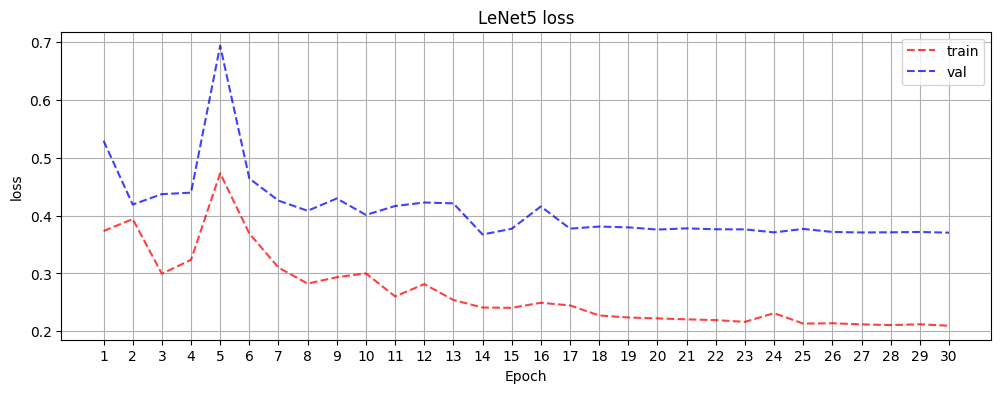
\includegraphics[width=0.95\linewidth]{graphics-raw/raw-loss-train_val.png}
    \caption{Loss en los conjuntos de entrenamiento y validación a lo largo de las épocas.}
    \label{fig:raw-loss-train_val}
\end{figure}
\noindent\textit{
En la Figura~\ref{fig:raw-loss-train_val} se observa la evolución de la función de pérdida (loss) para entrenamiento y validación. Ambas curvas descienden y se estabilizan, con la de entrenamiento alcanzando valores más bajos. La diferencia entre ambas no es significativa, lo que indica que el modelo no está sobreajustando y que la capacidad de generalización es adecuada.
}

\begin{figure}[H]
    \centering
    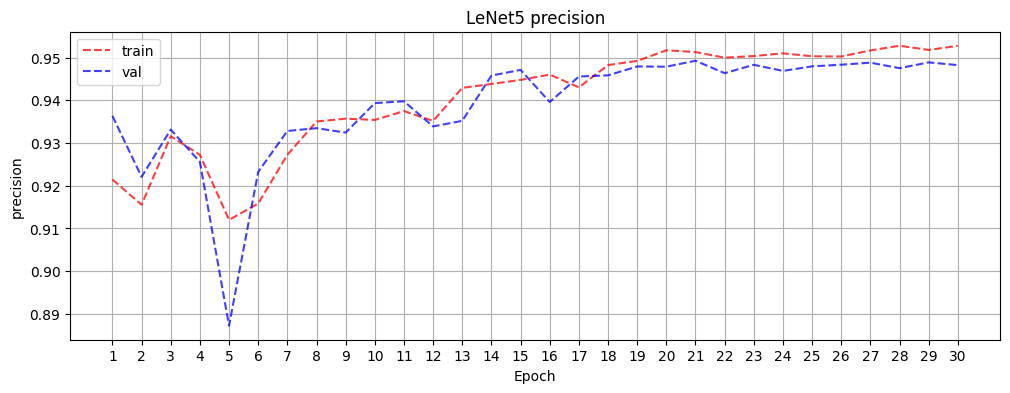
\includegraphics[width=0.95\linewidth]{graphics-raw/raw-precision-train_val.png}
    \caption{Precisión en los conjuntos de entrenamiento y validación a lo largo de las épocas.}
    \label{fig:raw-precision-train_val}
\end{figure}
\noindent\textit{
La Figura~\ref{fig:raw-precision-train_val} muestra que la precisión aumenta de manera constante durante el entrenamiento, con valores finales cercanos a 0.96 para ambos conjuntos. La similitud entre ambas curvas indica que el modelo es consistente y robusto en términos de precisión.
}

\begin{figure}[H]
    \centering
    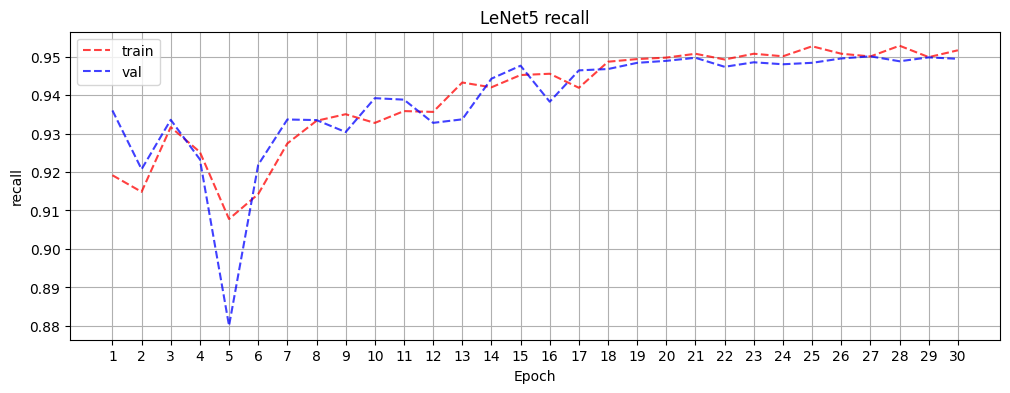
\includegraphics[width=0.95\linewidth]{graphics-raw/raw-recall-train_val.png}
    \caption{Recall en los conjuntos de entrenamiento y validación a lo largo de las épocas.}
    \label{fig:raw-recall-train_val}
\end{figure}
\noindent\textit{
Finalmente, la Figura~\ref{fig:raw-recall-train_val} muestra la evolución del recall durante el entrenamiento. Ambas curvas presentan una tendencia ascendente y convergente, alcanzando valores cercanos a 0.96. Esto indica que el modelo es capaz de identificar correctamente la mayoría de las instancias en ambos conjuntos, validando la robustez del entrenamiento y la selección de hiperparámetros.
}

% --- TEST ---

\begin{figure}[H]
    \centering
    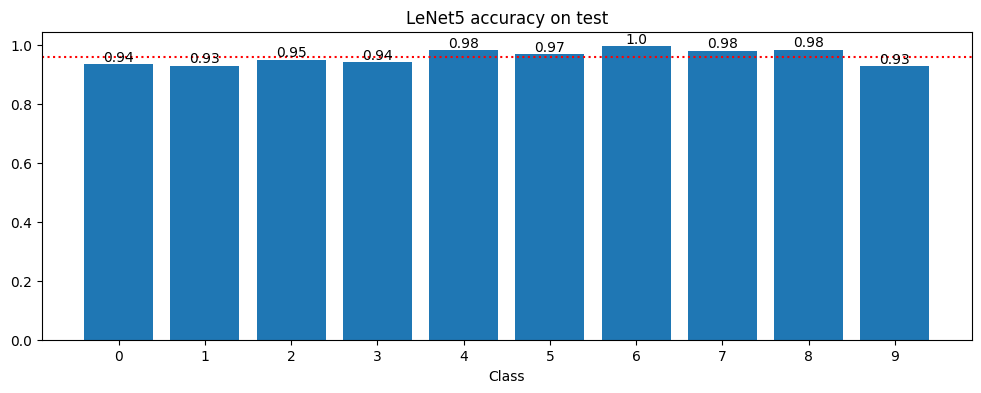
\includegraphics[width=0.95\linewidth]{graphics-raw/raw-accuracy-test.png}
    \caption{Accuracy por clase en el conjunto de prueba.}
    \label{fig:raw-accuracy-test}
\end{figure}
\noindent\textit{
En la Figura~\ref{fig:raw-accuracy-test} se observa que la precisión del modelo LeNet5 es alta y bastante uniforme entre las diferentes clases, con valores superiores a 0.93 en todas las clases y alcanzando 1.0 en la clase 6. La línea roja punteada indica el promedio general de accuracy. Este resultado evidencia que el modelo logra un desempeño sobresaliente y balanceado en la clasificación de los dígitos.
}

\begin{figure}[H]
    \centering
    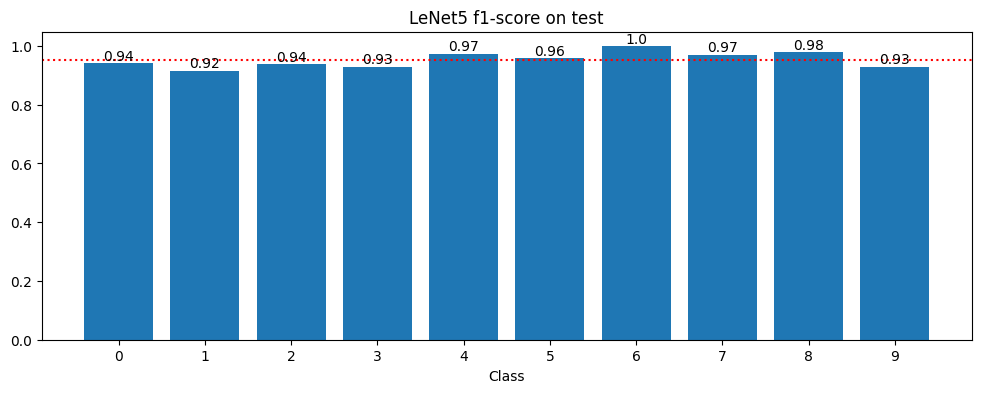
\includegraphics[width=0.95\linewidth]{graphics-raw/raw-f1score-test.png}
    \caption{F1-score por clase en el conjunto de prueba.}
    \label{fig:raw-f1score-test}
\end{figure}
\noindent\textit{
La Figura~\ref{fig:raw-f1score-test} muestra el F1-score por clase, con valores muy altos y consistentes en todas las clases, lo que indica que el modelo mantiene un excelente equilibrio entre precisión y recall. El F1-score promedio está representado por la línea roja punteada. Este comportamiento confirma la efectividad del modelo para este dataset.
}

\begin{figure}[H]
    \centering
    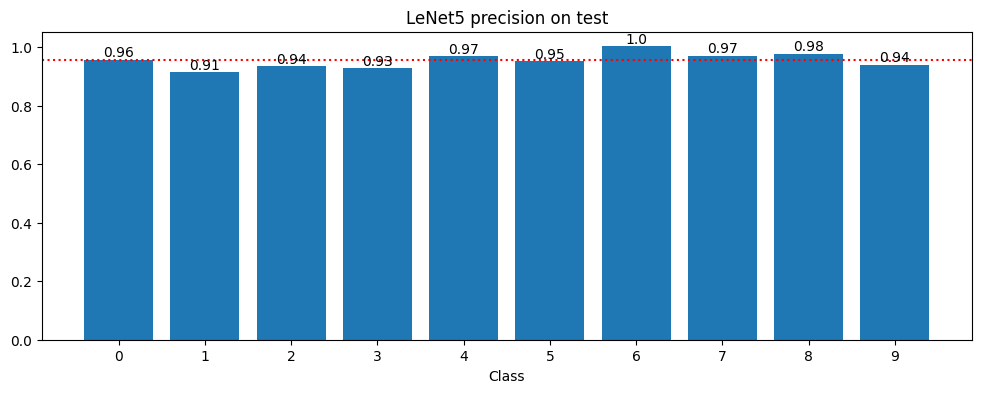
\includegraphics[width=0.95\linewidth]{graphics-raw/raw-precision-test.png}
    \caption{Precisión por clase en el conjunto de prueba.}
    \label{fig:raw-precision-test}
\end{figure}
\noindent\textit{
La Figura~\ref{fig:raw-precision-test} muestra la precisión por clase, con valores superiores a 0.91 en todas las clases y alcanzando 1.0 en la clase 6. Esto sugiere que el modelo es especialmente confiable para todas las clases, con un desempeño sobresaliente en la mayoría de ellas.
}

\begin{figure}[H]
    \centering
    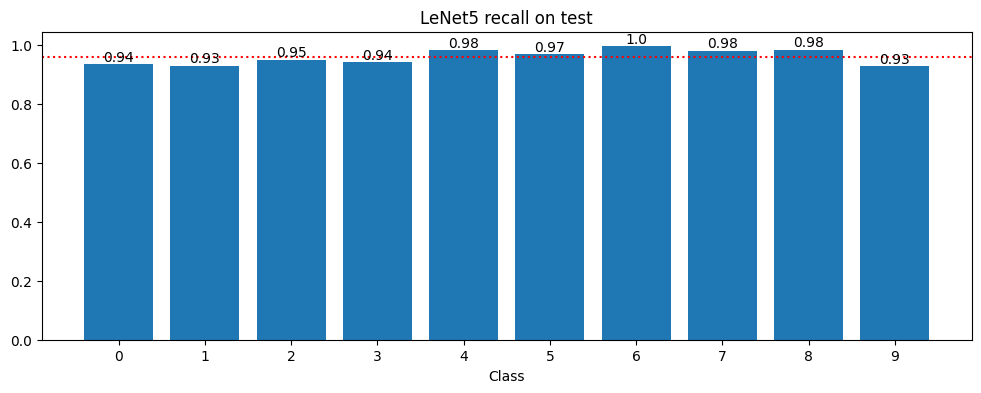
\includegraphics[width=0.95\linewidth]{graphics-raw/raw-recall-test.png}
    \caption{Recall por clase en el conjunto de prueba.}
    \label{fig:raw-recall-test}
\end{figure}
\noindent\textit{
La Figura~\ref{fig:raw-recall-test} muestra el recall por clase, con valores muy altos y consistentes, lo que indica que el modelo identifica correctamente la mayoría de las instancias de cada clase. El desempeño es especialmente alto en la clase 6, donde el recall es perfecto.
}

% --- MATRIZ DE CONFUSIÓN ---

\begin{figure}[H]
    \centering
    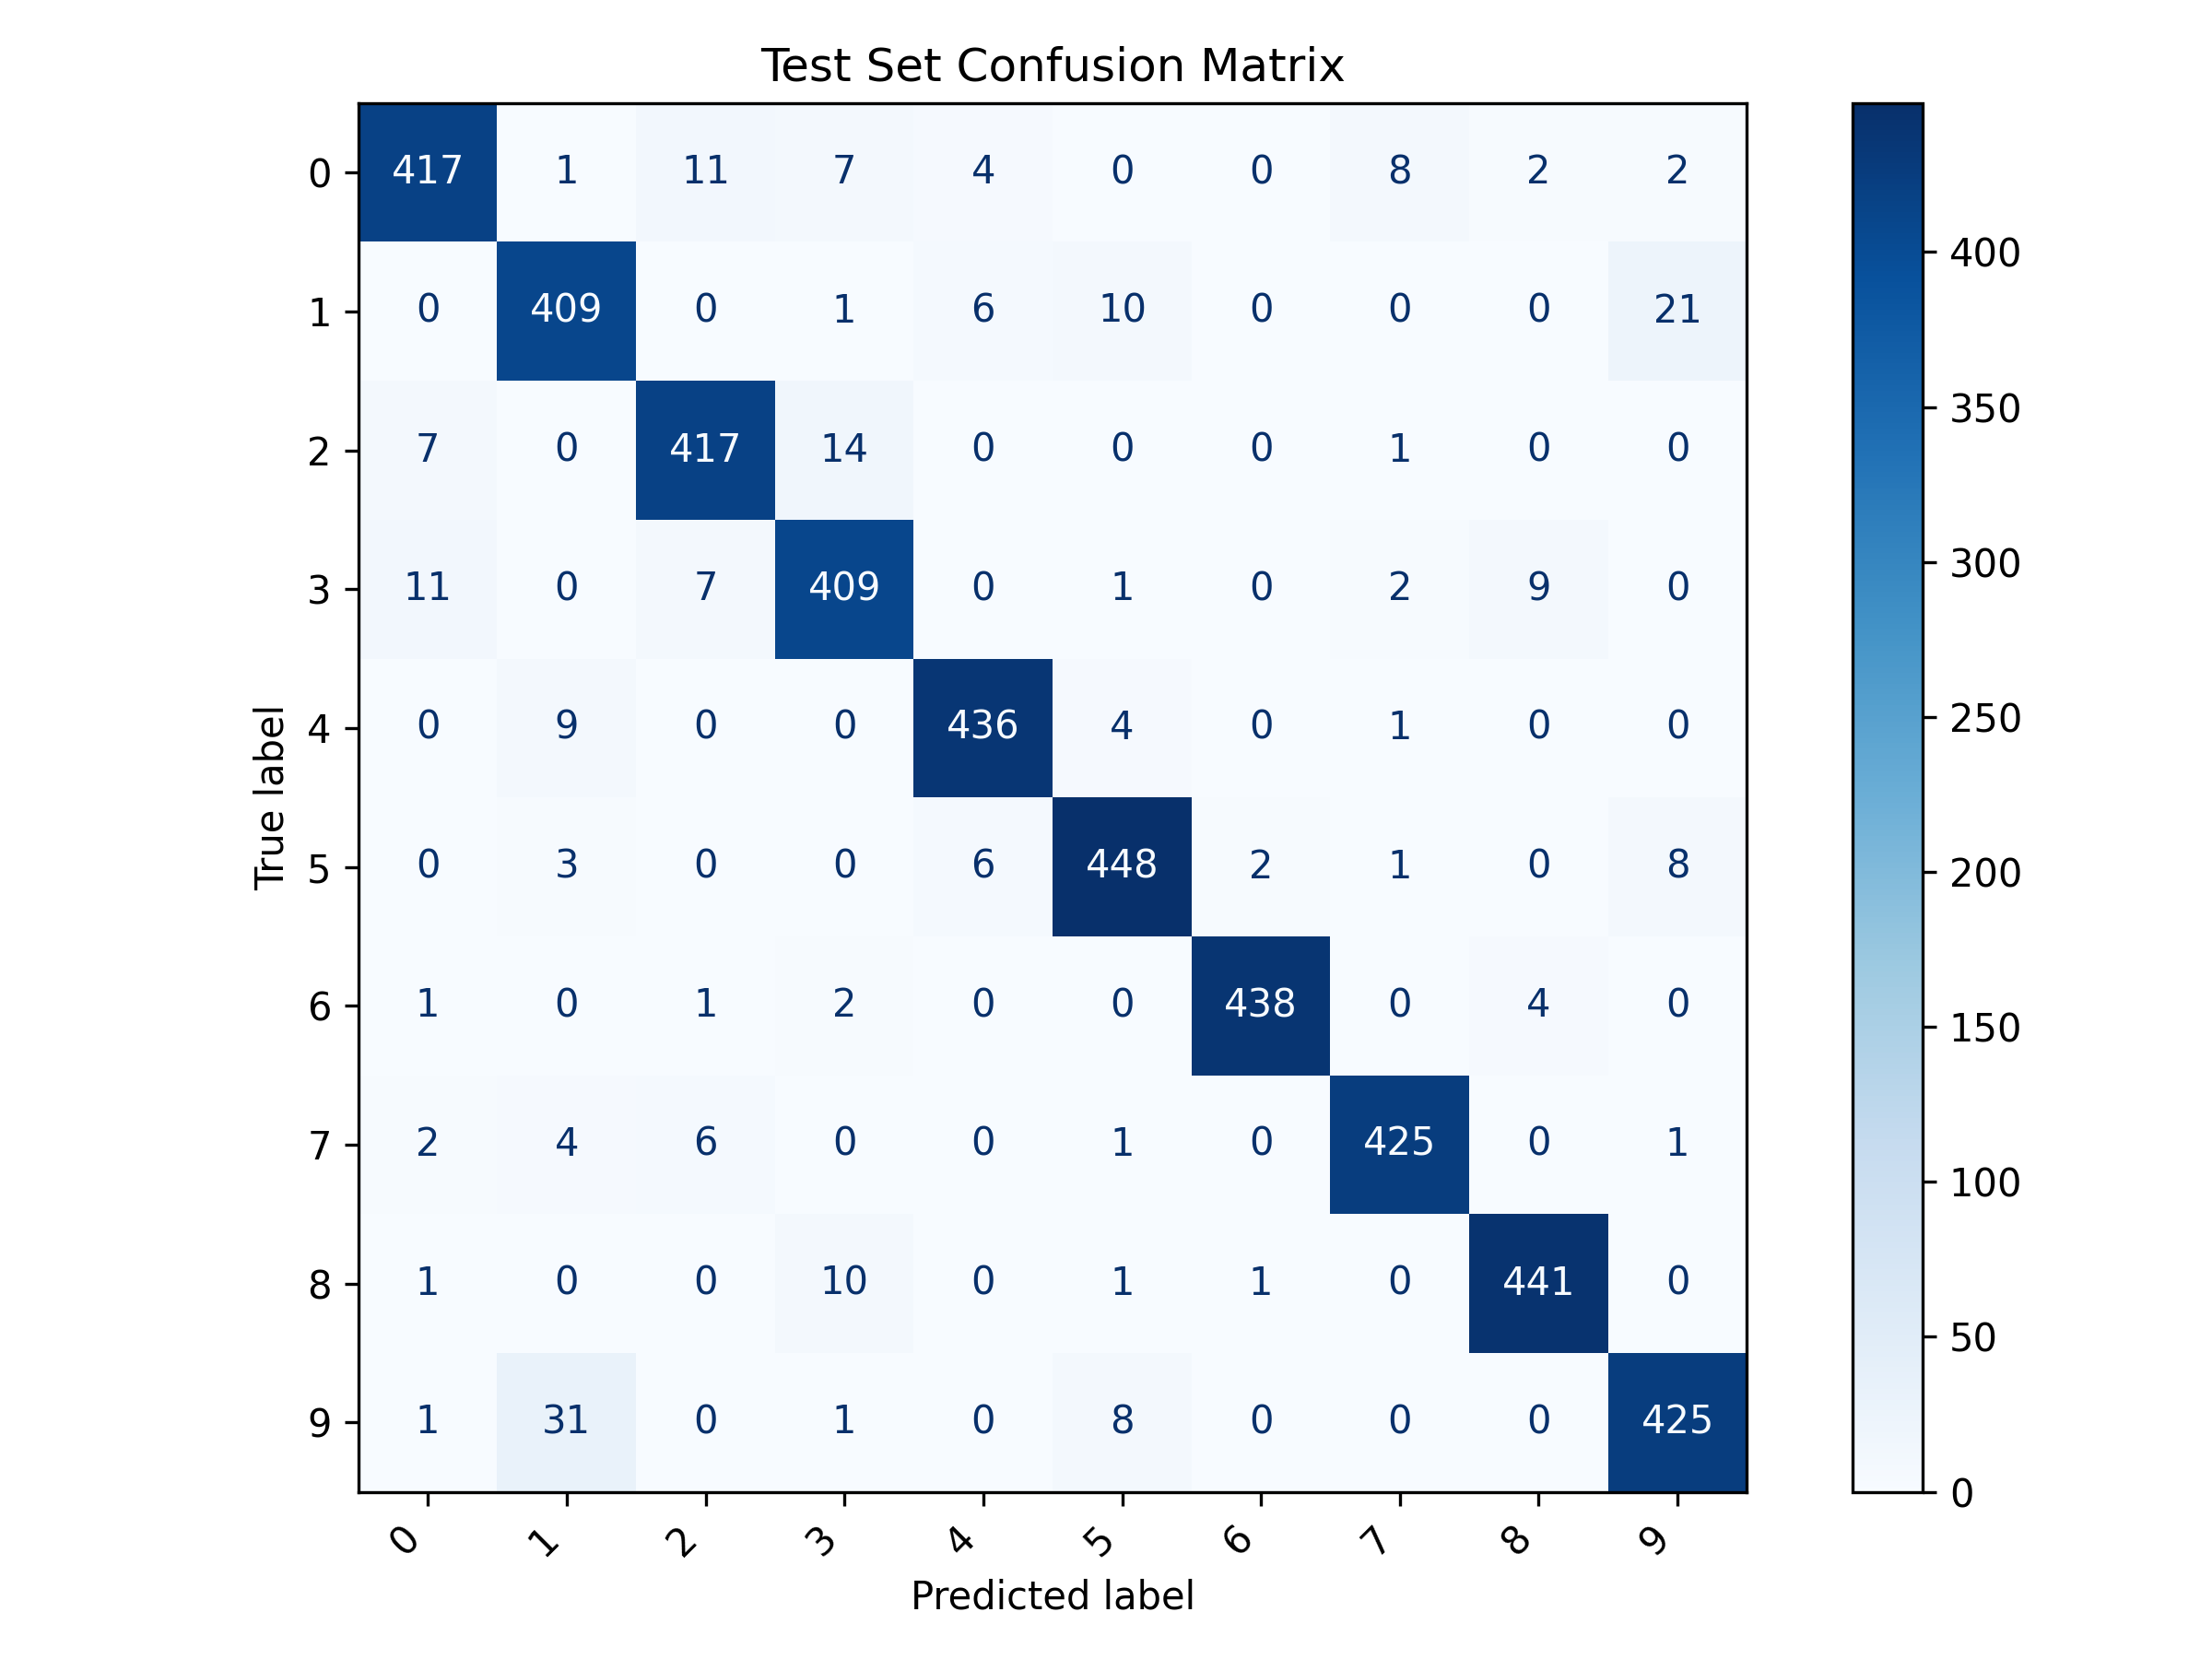
\includegraphics[width=0.95\linewidth]{graphics-raw/raw-confusion-matrix.png}
    \caption{Matriz de confusión del conjunto de prueba para Raw without Data Augmentation.}
    \label{fig:raw-confusion-matrix}
\end{figure}
\noindent\textit{
La Figura~\ref{fig:raw-confusion-matrix} muestra la matriz de confusión obtenida en el conjunto de prueba. Se observa que la mayoría de las predicciones se concentran en la diagonal principal, lo que indica un excelente desempeño general del modelo. Las confusiones entre clases son mínimas, aunque se puede notar que la clase 9 es confundida con la clase 1 en 31 ocasiones. Este resultado sugiere que el modelo es altamente preciso y robusto.
}


\subsubsection{Bilateral Filter without Data Augmentation}
Se realizaron 9 corridas con los hiperparámetros que se muestran en la Tabla~\ref{tab:bilateral_noaug_hparams}.

\begin{table}[H]
\caption{Hiperparámetros de las corridas (Bilateral Filter without Data Augmentation)}
\centering
\begin{tabular}{|c|c|c|}
\hline
\textbf{Corrida} & \textbf{Learning Rate} & \textbf{Epochs} \\
\hline
1 & 0.0001 & 15 \\
2 & 0.0005 & 15 \\
3 & 0.0007 & 15 \\
4 & 0.0007 & 20 \\
5 & 0.0007 & 25 \\
6 & 0.0008 & 20 \\
7 & 0.0008 & 25 \\
8 & 0.0008 & 20 \\
9 & 0.0008 & 25 \\
\hline
\end{tabular}
\label{tab:bilateral_noaug_hparams}
\end{table}

Los resultados de cada corrida se pueden observar en la Tabla~\ref{tab:bilateral_noaug_results} del Apéndice~\ref{appendix:results}.

\noindent\textit{
La Tabla~\ref{tab:bilateral_noaug_results} muestra que, aunque hay fluctuaciones en las métricas a lo largo de las corridas, la corrida 6 presenta los mejores resultados en accuracy, F1-score, precisión y recall para los conjuntos de prueba y validación, así como la menor pérdida (loss) en el conjunto de entrenamiento. Esto sugiere que el modelo se beneficia de un learning rate de 0.0008 y 20 épocas, logrando un equilibrio entre aprendizaje y generalización. Sin embargo, se observa que el modelo podría beneficiarse de un mayor ajuste de hiperparámetros para reducir la variabilidad entre corridas.
}

\subsection{Gráficas de Bilateral Filter without Data Augmentation}

A continuación se presentan las gráficas de las métricas obtenidas para el dataset \textit{Bilateral Filter without Data Augmentation}. Se muestran primero las métricas de entrenamiento y validación, seguidas de las métricas por clase en el conjunto de prueba y, finalmente, la matriz de confusión.

% --- TRAIN/VAL ---

\begin{figure}[H]
    \centering
    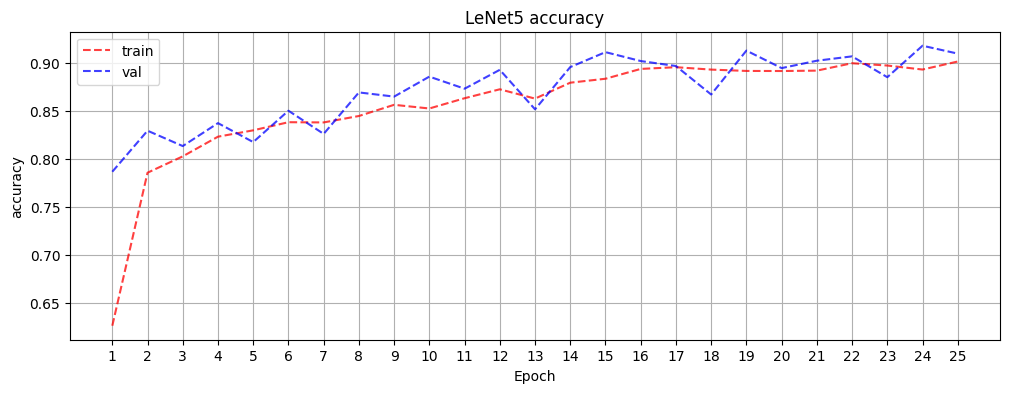
\includegraphics[width=0.95\linewidth]{graphics-bilateral/bilateral-accuracy-train_val.png}
    \caption{Accuracy en los conjuntos de entrenamiento y validación a lo largo de las épocas.}
    \label{fig:bilateral-accuracy-train_val}
\end{figure}
\noindent\textit{
La Figura~\ref{fig:bilateral-accuracy-train_val} muestra la evolución del accuracy durante el entrenamiento. Se observa una tendencia ascendente y una convergencia entre las curvas de entrenamiento y validación, alcanzando valores cercanos a 0.92. La curva de validación se mantiene ligeramente por encima de la de entrenamiento en varias épocas, lo que indica una buena capacidad de generalización y ausencia de sobreajuste significativo.
}

\begin{figure}[H]
    \centering
    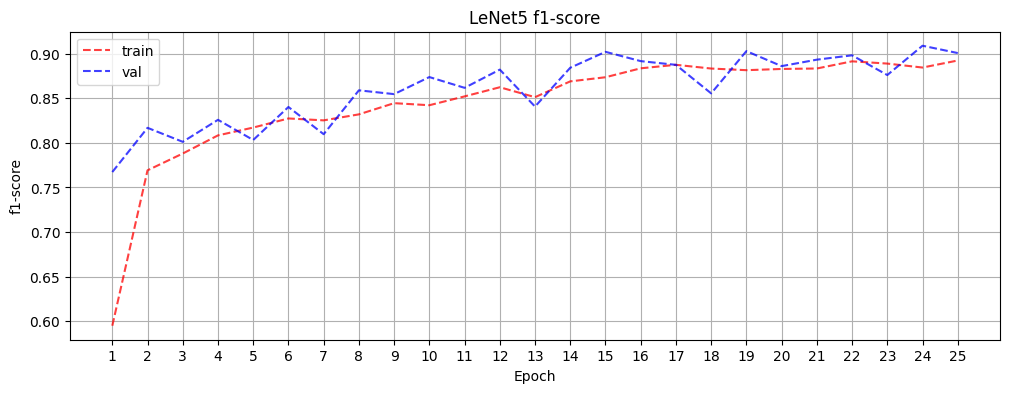
\includegraphics[width=0.95\linewidth]{graphics-bilateral/bilateral-f1score-train_val.png}
    \caption{F1-score en los conjuntos de entrenamiento y validación a lo largo de las épocas.}
    \label{fig:bilateral-f1score-train_val}
\end{figure}
\noindent\textit{
La Figura~\ref{fig:bilateral-f1score-train_val} muestra la evolución del F1-score durante el entrenamiento. Ambas curvas presentan una mejora progresiva y se mantienen cercanas, alcanzando valores superiores a 0.9. Esto indica que el modelo mantiene un buen equilibrio entre precisión y recall, y que la selección de hiperparámetros es adecuada para este preprocesamiento.
}

\begin{figure}[H]
    \centering
    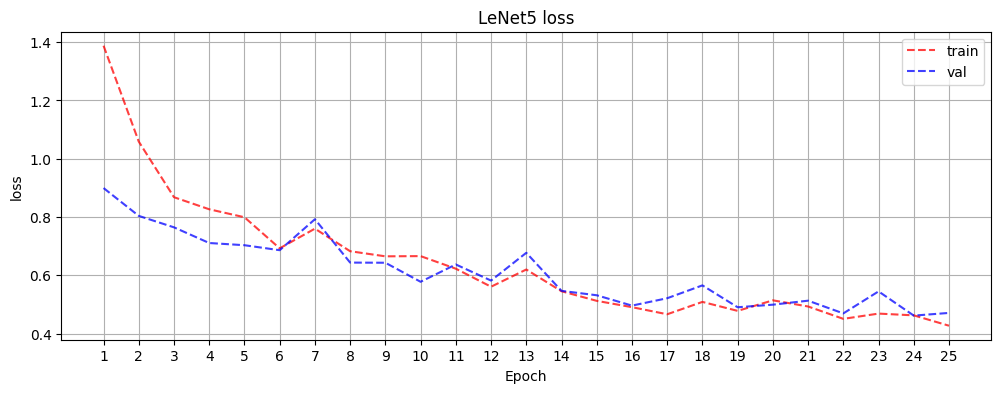
\includegraphics[width=0.95\linewidth]{graphics-bilateral/bilateral-loss-train_val.png}
    \caption{Loss en los conjuntos de entrenamiento y validación a lo largo de las épocas.}
    \label{fig:bilateral-loss-train_val}
\end{figure}
\noindent\textit{
En la Figura~\ref{fig:bilateral-loss-train_val} se observa la evolución de la función de pérdida (loss) para entrenamiento y validación. Ambas curvas descienden y se estabilizan, con la de validación ligeramente por encima de la de entrenamiento. Esto indica que el modelo no está sobreajustando y que la capacidad de generalización es adecuada.
}

\begin{figure}[H]
    \centering
    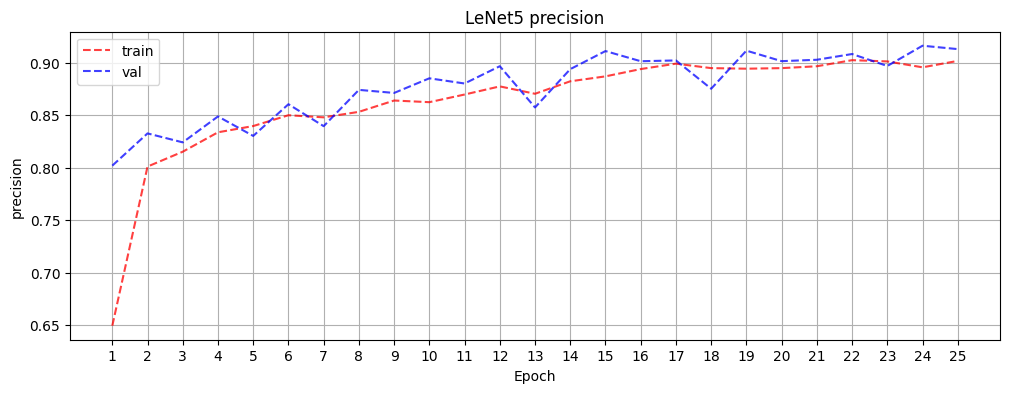
\includegraphics[width=0.95\linewidth]{graphics-bilateral/bilateral-precision-train_val.png}
    \caption{Precisión en los conjuntos de entrenamiento y validación a lo largo de las épocas.}
    \label{fig:bilateral-precision-train_val}
\end{figure}
\noindent\textit{
La Figura~\ref{fig:bilateral-precision-train_val} muestra que la precisión aumenta de manera constante durante el entrenamiento, con valores finales cercanos a 0.92 para ambos conjuntos. La similitud entre ambas curvas indica que el modelo es consistente y robusto en términos de precisión, lo que es un resultado positivo para la generalización.
}

\begin{figure}[H]
    \centering
    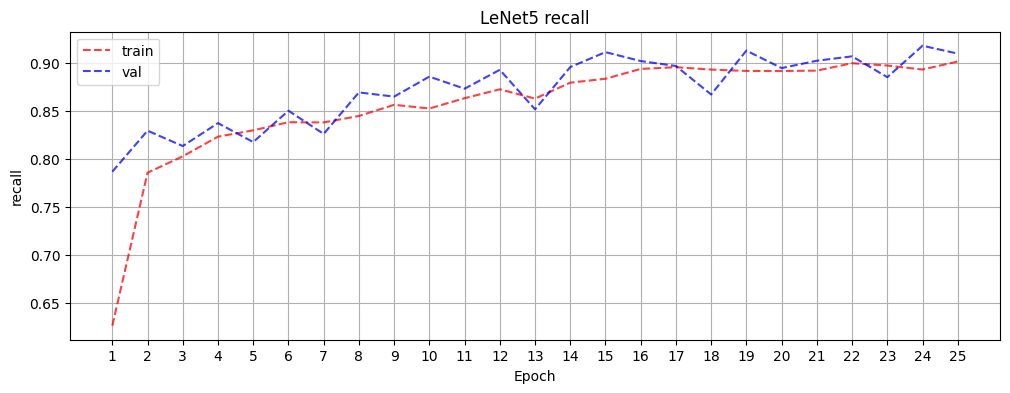
\includegraphics[width=0.95\linewidth]{graphics-bilateral/bilateral-recall-train_val.png}
    \caption{Recall en los conjuntos de entrenamiento y validación a lo largo de las épocas.}
    \label{fig:bilateral-recall-train_val}
\end{figure}
\noindent\textit{
Finalmente, la Figura~\ref{fig:bilateral-recall-train_val} muestra la evolución del recall durante el entrenamiento. Ambas curvas presentan una tendencia ascendente y convergente, alcanzando valores cercanos a 0.92. Esto indica que el modelo es capaz de identificar correctamente la mayoría de las instancias en ambos conjuntos, validando la robustez del entrenamiento y la selección de hiperparámetros.
}

% --- TEST ---

\begin{figure}[H]
    \centering
    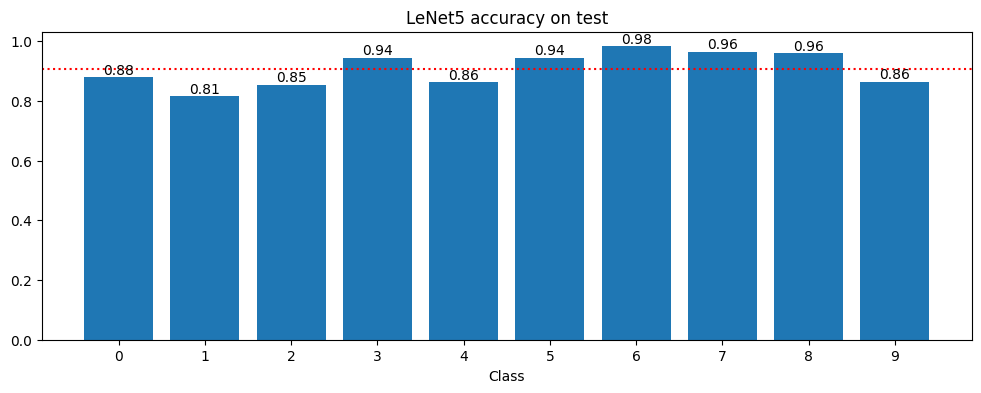
\includegraphics[width=0.95\linewidth]{graphics-bilateral/bilateral-accuracy-test.png}
    \caption{Accuracy por clase en el conjunto de prueba.}
    \label{fig:bilateral-accuracy-test}
\end{figure}
\noindent\textit{
En la Figura~\ref{fig:bilateral-accuracy-test} se observa que la precisión del modelo LeNet5 es alta y bastante uniforme entre las diferentes clases, con valores superiores a 0.81 en todas las clases y alcanzando 0.98 en la clase 6. La línea roja punteada indica el promedio general de accuracy. Este resultado evidencia que el modelo logra un desempeño sobresaliente y balanceado en la clasificación de los dígitos, aunque la clase 1 presenta el menor desempeño relativo.
}

\begin{figure}[H]
    \centering
    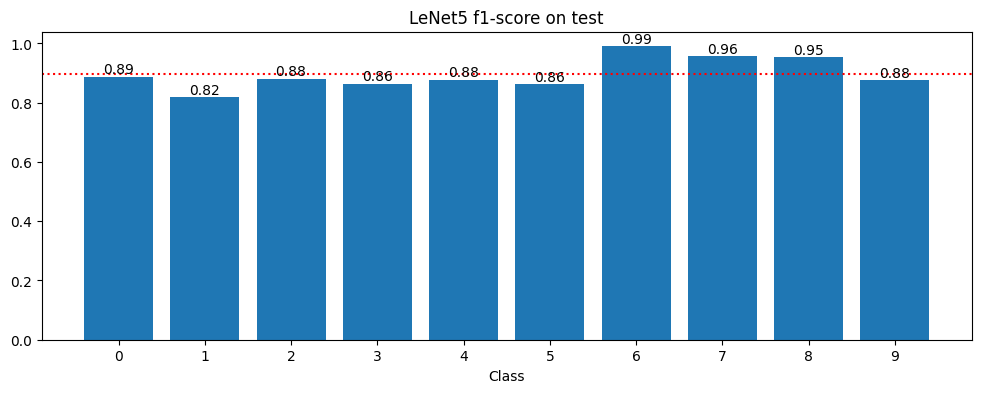
\includegraphics[width=0.95\linewidth]{graphics-bilateral/bilateral-f1score-test.png}
    \caption{F1-score por clase en el conjunto de prueba.}
    \label{fig:bilateral-f1score-test}
\end{figure}
\noindent\textit{
La Figura~\ref{fig:bilateral-f1score-test} muestra el F1-score por clase, con valores muy altos y consistentes en todas las clases, lo que indica que el modelo mantiene un excelente equilibrio entre precisión y recall. El F1-score promedio está representado por la línea roja punteada. Este comportamiento confirma la efectividad del modelo para este dataset, aunque la clase 1 sigue siendo la más desafiante.
}

\begin{figure}[H]
    \centering
    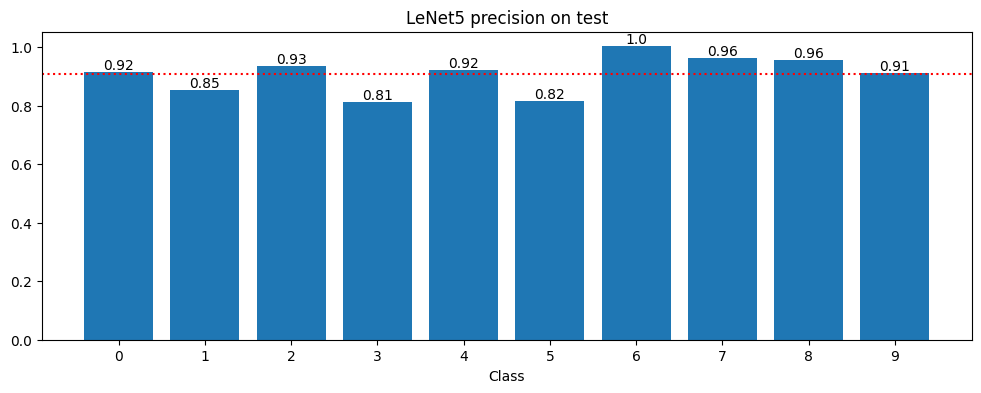
\includegraphics[width=0.95\linewidth]{graphics-bilateral/bilateral-precision-test.png}
    \caption{Precisión por clase en el conjunto de prueba.}
    \label{fig:bilateral-precision-test}
\end{figure}
\noindent\textit{
La Figura~\ref{fig:bilateral-precision-test} muestra la precisión por clase, con valores superiores a 0.81 en todas las clases y alcanzando 1.0 en la clase 6. Esto sugiere que el modelo es especialmente confiable para todas las clases, con un desempeño sobresaliente en la mayoría de ellas, aunque la clase 3 presenta el menor valor de precisión.
}

\begin{figure}[H]
    \centering
    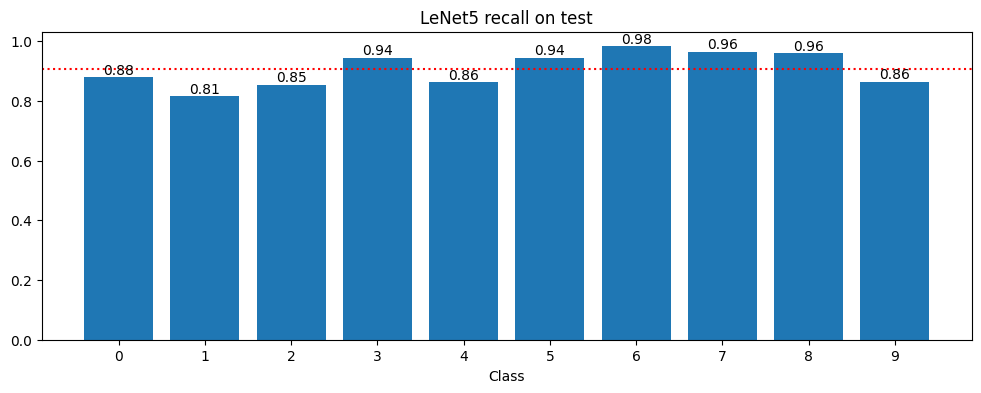
\includegraphics[width=0.95\linewidth]{graphics-bilateral/bilateral-recall-test.png}
    \caption{Recall por clase en el conjunto de prueba.}
    \label{fig:bilateral-recall-test}
\end{figure}
\noindent\textit{
La Figura~\ref{fig:bilateral-recall-test} muestra el recall por clase, con valores muy altos y consistentes, lo que indica que el modelo identifica correctamente la mayoría de las instancias de cada clase. El desempeño es especialmente alto en la clase 6, donde el recall es cercano a 1.0, mientras que la clase 1 presenta el menor valor de recall.
}

% --- MATRIZ DE CONFUSIÓN ---

\begin{figure}[H]
    \centering
    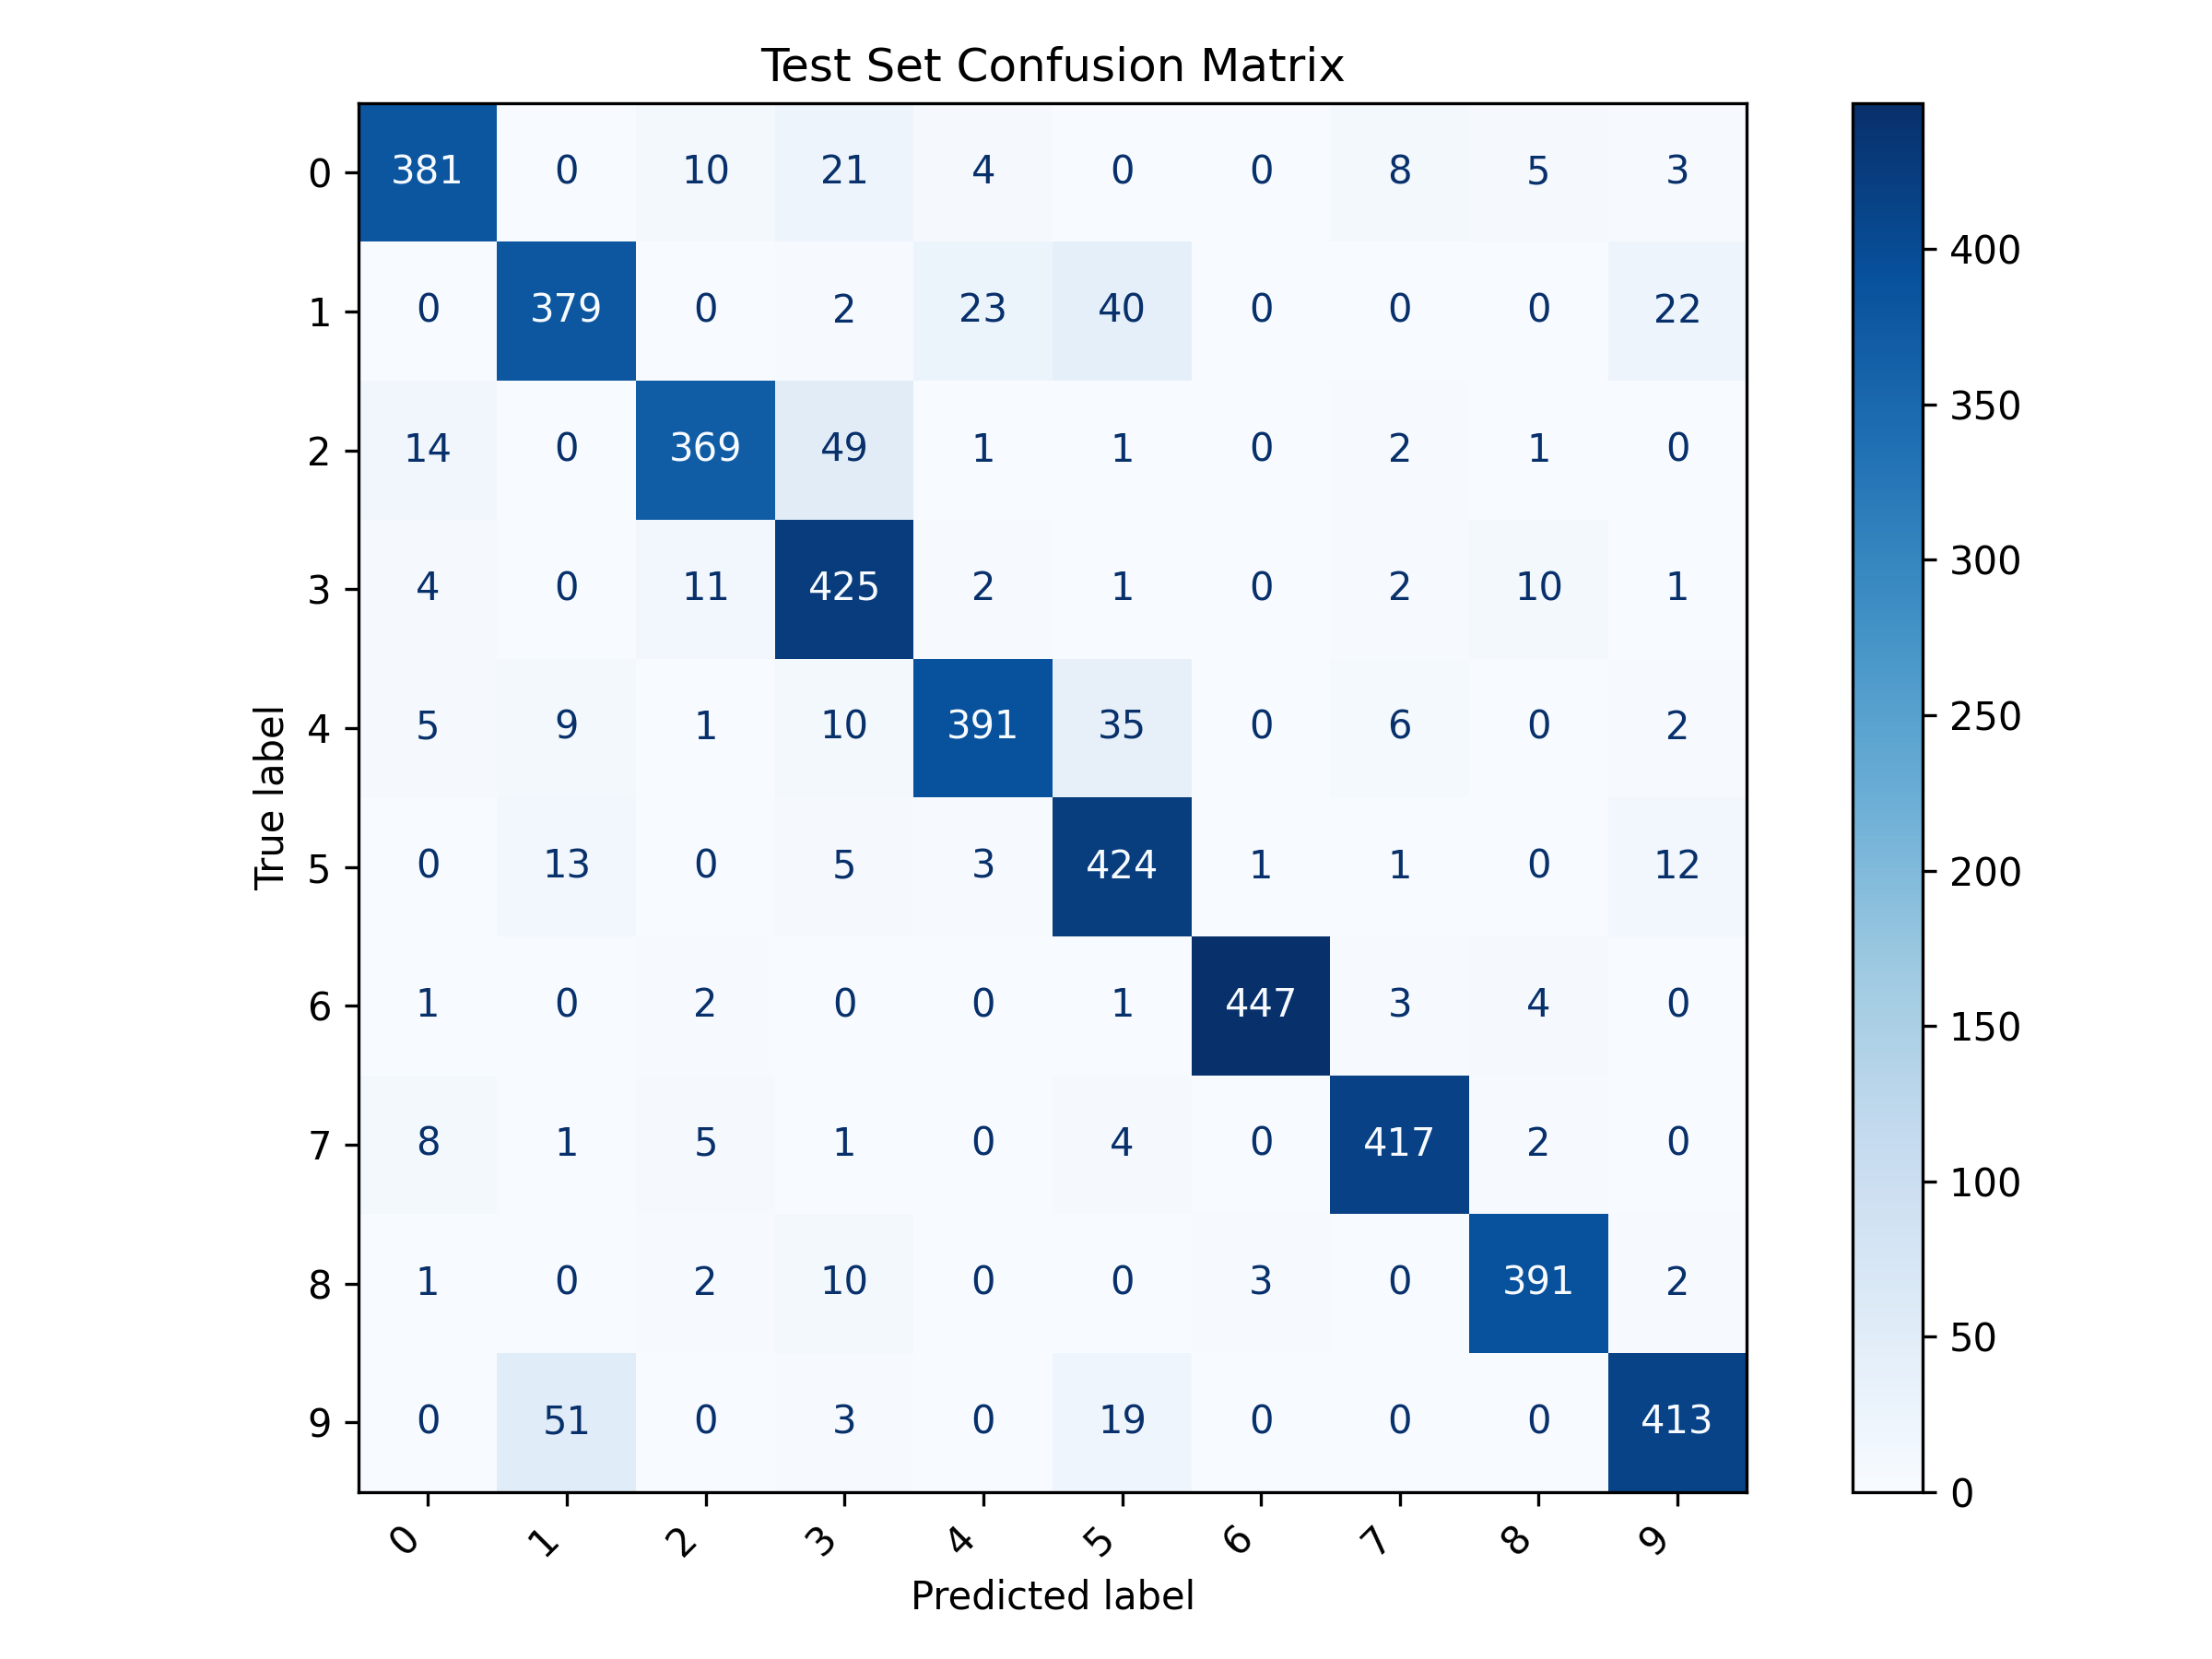
\includegraphics[width=0.95\linewidth]{graphics-bilateral/bilateral-confusion-matrix.png}
    \caption{Matriz de confusión del conjunto de prueba para Bilateral Filter without Data Augmentation.}
    \label{fig:bilateral-confusion-matrix}
\end{figure}
\noindent\textit{
La Figura~\ref{fig:bilateral-confusion-matrix} muestra la matriz de confusión obtenida en el conjunto de prueba. Se observa que la mayoría de las predicciones se concentran en la diagonal principal, lo que indica un excelente desempeño general del modelo. Las confusiones entre clases son mínimas, aunque se puede notar que la clase 9 es confundida con la clase 1 en 51 ocasiones y la clase 2 con la clase 3 en 49 ocasiones. Este resultado sugiere que el modelo es altamente preciso y robusto.
}


\subsubsection{Bilateral Filter with Data Augmentation}
Se realizaron 7 corridas con los hiperparámetros que se muestran en la Tabla~\ref{tab:bilateral_aug_hparams}.

\begin{table}[H]
\caption{Hiperparámetros de las corridas (Bilateral Filter with Data Augmentation)}
\centering
\begin{tabular}{|c|c|c|}
\hline
\textbf{Corrida} & \textbf{Learning Rate} & \textbf{Epochs} \\
\hline
1 & 0.0001 & 15 \\
2 & 0.0005 & 15 \\
3 & 0.0007 & 15 \\
4 & 0.0007 & 20 \\
5 & 0.0007 & 25 \\
6 & 0.0008 & 20 \\
7 & 0.0008 & 25 \\
\hline
\end{tabular}
\label{tab:bilateral_aug_hparams}
\end{table}

Los resultados de cada corrida se pueden observar en la Tabla~\ref{tab:bilateral_aug_results} del Apéndice~\ref{appendix:results}.

\noindent\textit{
En la Tabla~\ref{tab:bilateral_aug_results}, la corrida 6 destaca por obtener los mejores valores en la mayoría de las métricas, especialmente en accuracy, F1-score, precisión y recall en los tres conjuntos, así como la menor pérdida (loss) en el conjunto de entrenamiento. Esto indica que el modelo logra su mejor desempeño con un learning rate de 0.0008 y 20 épocas, lo que permite una mejor adaptación a los datos aumentados y una mayor capacidad de generalización. La consistencia de los resultados en esta corrida sugiere que estos hiperparámetros son los más adecuados para este preprocesamiento.
}

\subsection{Gráficas de Bilateral Filter with Data Augmentation}

A continuación se presentan las gráficas de las métricas obtenidas para el dataset \textit{Bilateral Filter with Data Augmentation}. Se muestran primero las métricas de entrenamiento y validación, seguidas de las métricas por clase en el conjunto de prueba y, finalmente, la matriz de confusión.

% --- TRAIN/VAL ---

\begin{figure}[H]
    \centering
    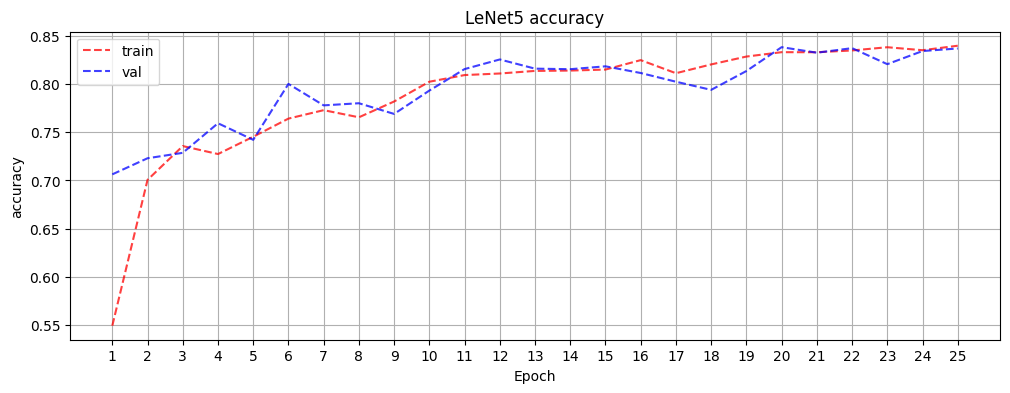
\includegraphics[width=0.95\linewidth]{graphics-bilateral-da/bilateral-da-accuracy-train_val.png}
    \caption{Accuracy en los conjuntos de entrenamiento y validación a lo largo de las épocas.}
    \label{fig:bilateral-da-accuracy-train_val}
\end{figure}
\noindent\textit{
La Figura~\ref{fig:bilateral-da-accuracy-train_val} muestra la evolución del accuracy durante el entrenamiento. Se observa una tendencia ascendente y una convergencia entre las curvas de entrenamiento y validación, alcanzando valores cercanos a 0.84. Aunque el desempeño es aceptable, los valores finales son inferiores a los obtenidos en los experimentos sin data augmentation.
}

\begin{figure}[H]
    \centering
    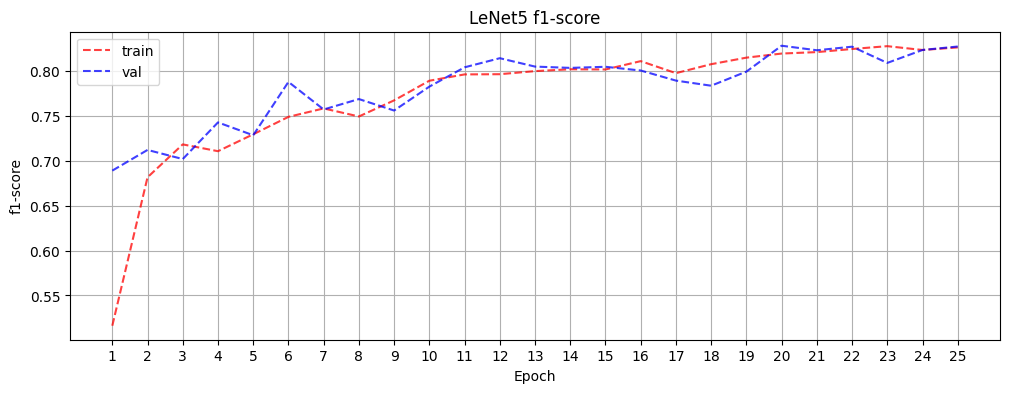
\includegraphics[width=0.95\linewidth]{graphics-bilateral-da/bilateral-da-f1score-train_val.png}
    \caption{F1-score en los conjuntos de entrenamiento y validación a lo largo de las épocas.}
    \label{fig:bilateral-da-f1score-train_val}
\end{figure}
\noindent\textit{
La Figura~\ref{fig:bilateral-da-f1score-train_val} muestra la evolución del F1-score durante el entrenamiento. Ambas curvas presentan una mejora progresiva y se mantienen cercanas, lo que indica que el modelo mantiene un equilibrio entre precisión y recall, aunque con valores finales moderados. Esto sugiere que el modelo generaliza razonablemente bien.
}

\begin{figure}[H]
    \centering
    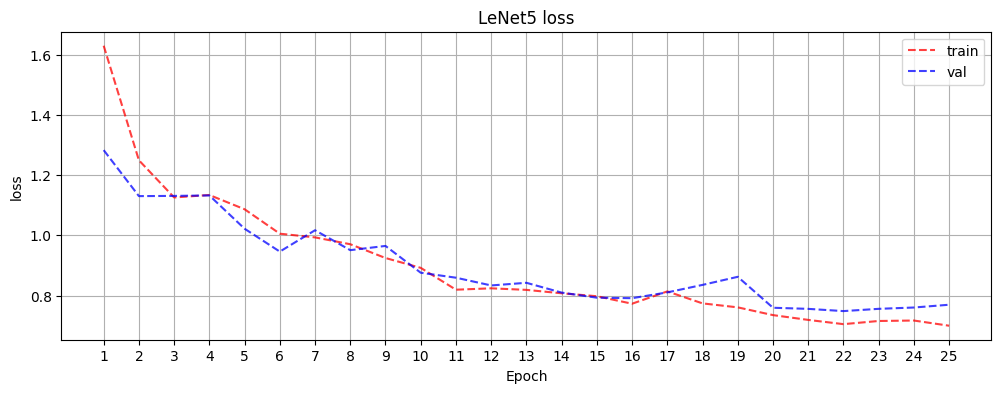
\includegraphics[width=0.95\linewidth]{graphics-bilateral-da/bilateral-da-loss-train_val.png}
    \caption{Loss en los conjuntos de entrenamiento y validación a lo largo de las épocas.}
    \label{fig:bilateral-da-loss-train_val}
\end{figure}
\noindent\textit{
En la Figura~\ref{fig:bilateral-da-loss-train_val} se observa la evolución de la función de pérdida (loss) para entrenamiento y validación. Ambas curvas descienden y se estabilizan, aunque la pérdida de validación se mantiene ligeramente por encima de la de entrenamiento. Esto indica que el modelo no está sobreajustando.
}

\begin{figure}[H]
    \centering
    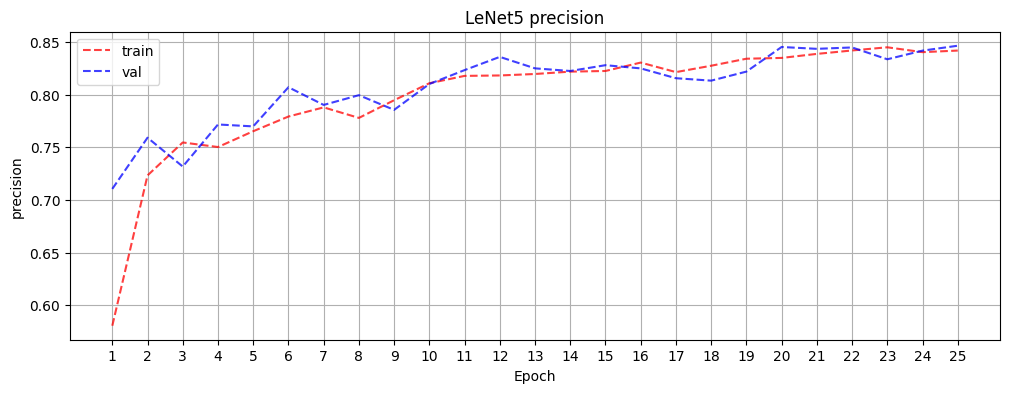
\includegraphics[width=0.95\linewidth]{graphics-bilateral-da/bilateral-da-precision-train_val.png}
    \caption{Precisión en los conjuntos de entrenamiento y validación a lo largo de las épocas.}
    \label{fig:bilateral-da-precision-train_val}
\end{figure}
\noindent\textit{
La Figura~\ref{fig:bilateral-da-precision-train_val} muestra que la precisión aumenta de manera constante durante el entrenamiento, con valores finales cercanos a 0.84 para ambos conjuntos. La similitud entre ambas curvas indica que el modelo es consistente y robusto en términos de precisión.
}

\begin{figure}[H]
    \centering
    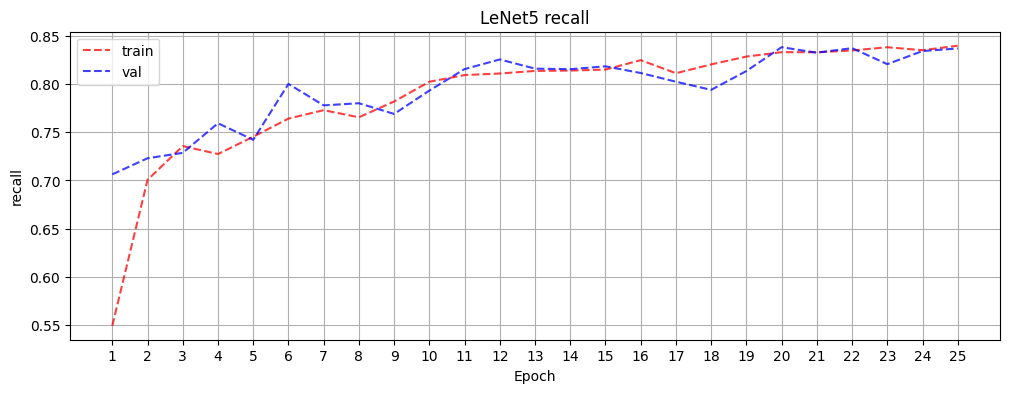
\includegraphics[width=0.95\linewidth]{graphics-bilateral-da/bilateral-da-recall-train_val.png}
    \caption{Recall en los conjuntos de entrenamiento y validación a lo largo de las épocas.}
    \label{fig:bilateral-da-recall-train_val}
\end{figure}
\noindent\textit{
Finalmente, la Figura~\ref{fig:bilateral-da-recall-train_val} muestra la evolución del recall durante el entrenamiento. Ambas curvas presentan una tendencia ascendente y convergente, alcanzando valores cercanos a 0.84. Esto indica que el modelo es capaz de identificar correctamente la mayoría de las instancias en ambos conjuntos, aunque el desempeño es menor que en los experimentos sin data augmentation y sin bilateral filter.
}

% --- TEST ---

\begin{figure}[H]
    \centering
    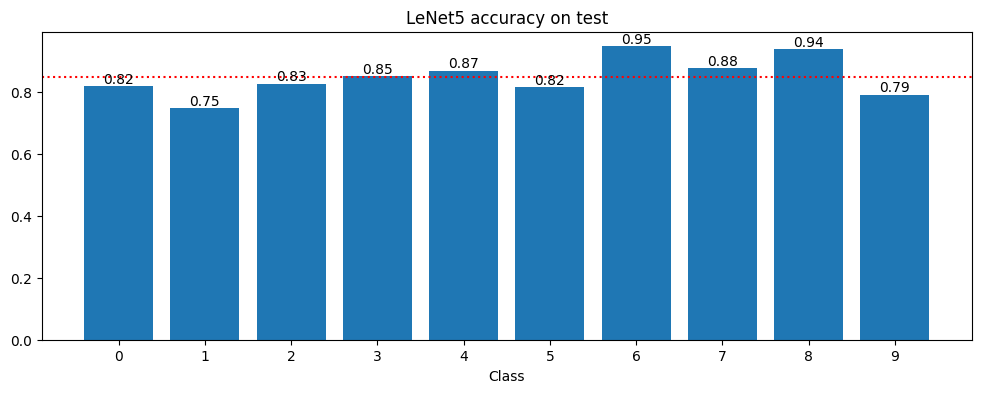
\includegraphics[width=0.95\linewidth]{graphics-bilateral-da/bilateral-da-accuracy-test.png}
    \caption{Accuracy por clase en el conjunto de prueba.}
    \label{fig:bilateral-da-accuracy-test}
\end{figure}
\noindent\textit{
En la Figura~\ref{fig:bilateral-da-accuracy-test} se observa que la precisión del modelo LeNet5 varía considerablemente entre las diferentes clases, con valores que van desde 0.75 hasta 0.95. Las clases 1 y 9 presentan los desempeños más bajos, lo que sugiere que el modelo tiene dificultades particulares con estas clases.
}

\begin{figure}[H]
    \centering
    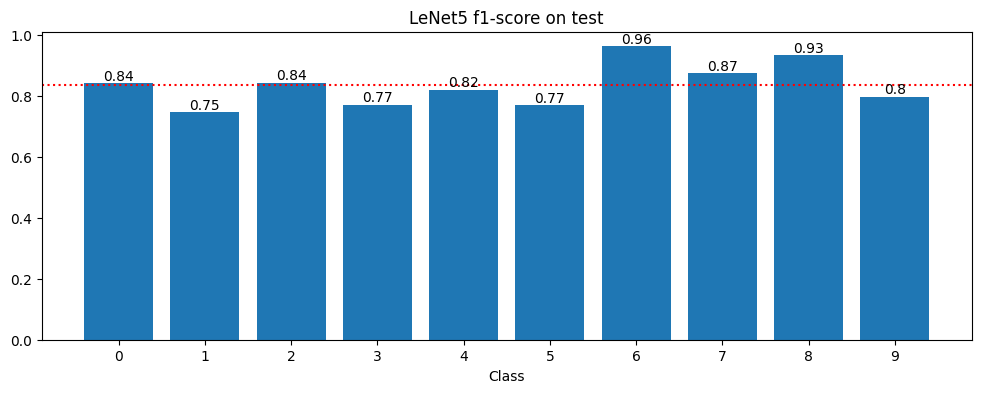
\includegraphics[width=0.95\linewidth]{graphics-bilateral-da/bilateral-da-f1score-test.png}
    \caption{F1-score por clase en el conjunto de prueba.}
    \label{fig:bilateral-da-f1score-test}
\end{figure}
\noindent\textit{
La Figura~\ref{fig:bilateral-da-f1score-test} muestra el F1-score por clase, con valores que reflejan la variabilidad observada en el accuracy. Las clases 1, 3, 5 y 9 presentan los valores más bajos, mientras que la clase 6 destaca con un F1-score de 0.96.
}

\begin{figure}[H]
    \centering
    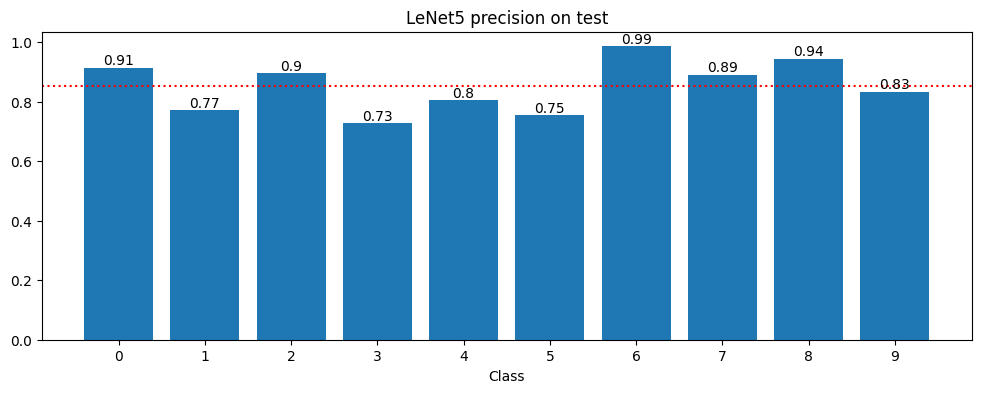
\includegraphics[width=0.95\linewidth]{graphics-bilateral-da/bilateral-da-precision-test.png}
    \caption{Precisión por clase en el conjunto de prueba.}
    \label{fig:bilateral-da-precision-test}
\end{figure}
\noindent\textit{
La Figura~\ref{fig:bilateral-da-precision-test} muestra la precisión por clase, con valores que oscilan entre 0.73 y 0.99. Las clases 3 y 5 presentan los valores más bajos, mientras que la clase 6 alcanza un valor cercano a 1.0. Estos resultados sugieren que el modelo es especialmente confiable para ciertas clases.
}

\begin{figure}[H]
    \centering
    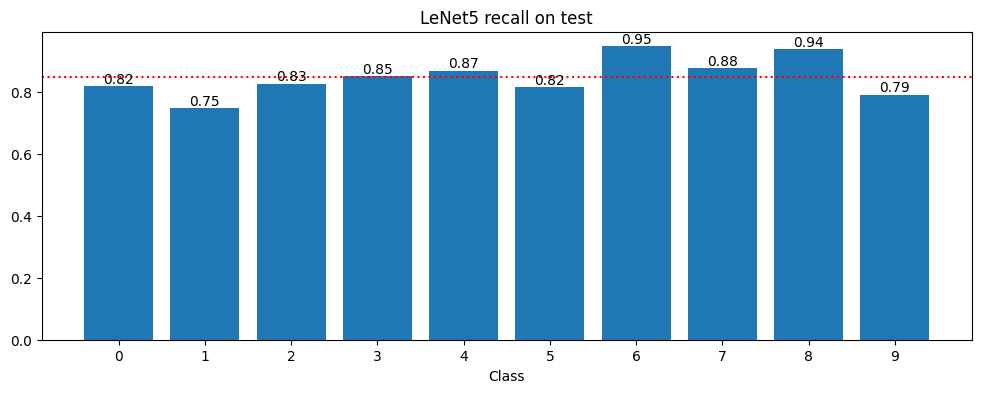
\includegraphics[width=0.95\linewidth]{graphics-bilateral-da/bilateral-da-recall-test.png}
    \caption{Recall por clase en el conjunto de prueba.}
    \label{fig:bilateral-da-recall-test}
\end{figure}
\noindent\textit{
La Figura~\ref{fig:bilateral-da-recall-test} muestra el recall por clase, con valores que reflejan la variabilidad observada en las otras métricas. Las clases 1 y 9 presentan los valores más bajos, lo que indica que el modelo tiene dificultades para identificar correctamente todas las instancias de estas clases.
}

% --- MATRIZ DE CONFUSIÓN ---

\begin{figure}[H]
    \centering
    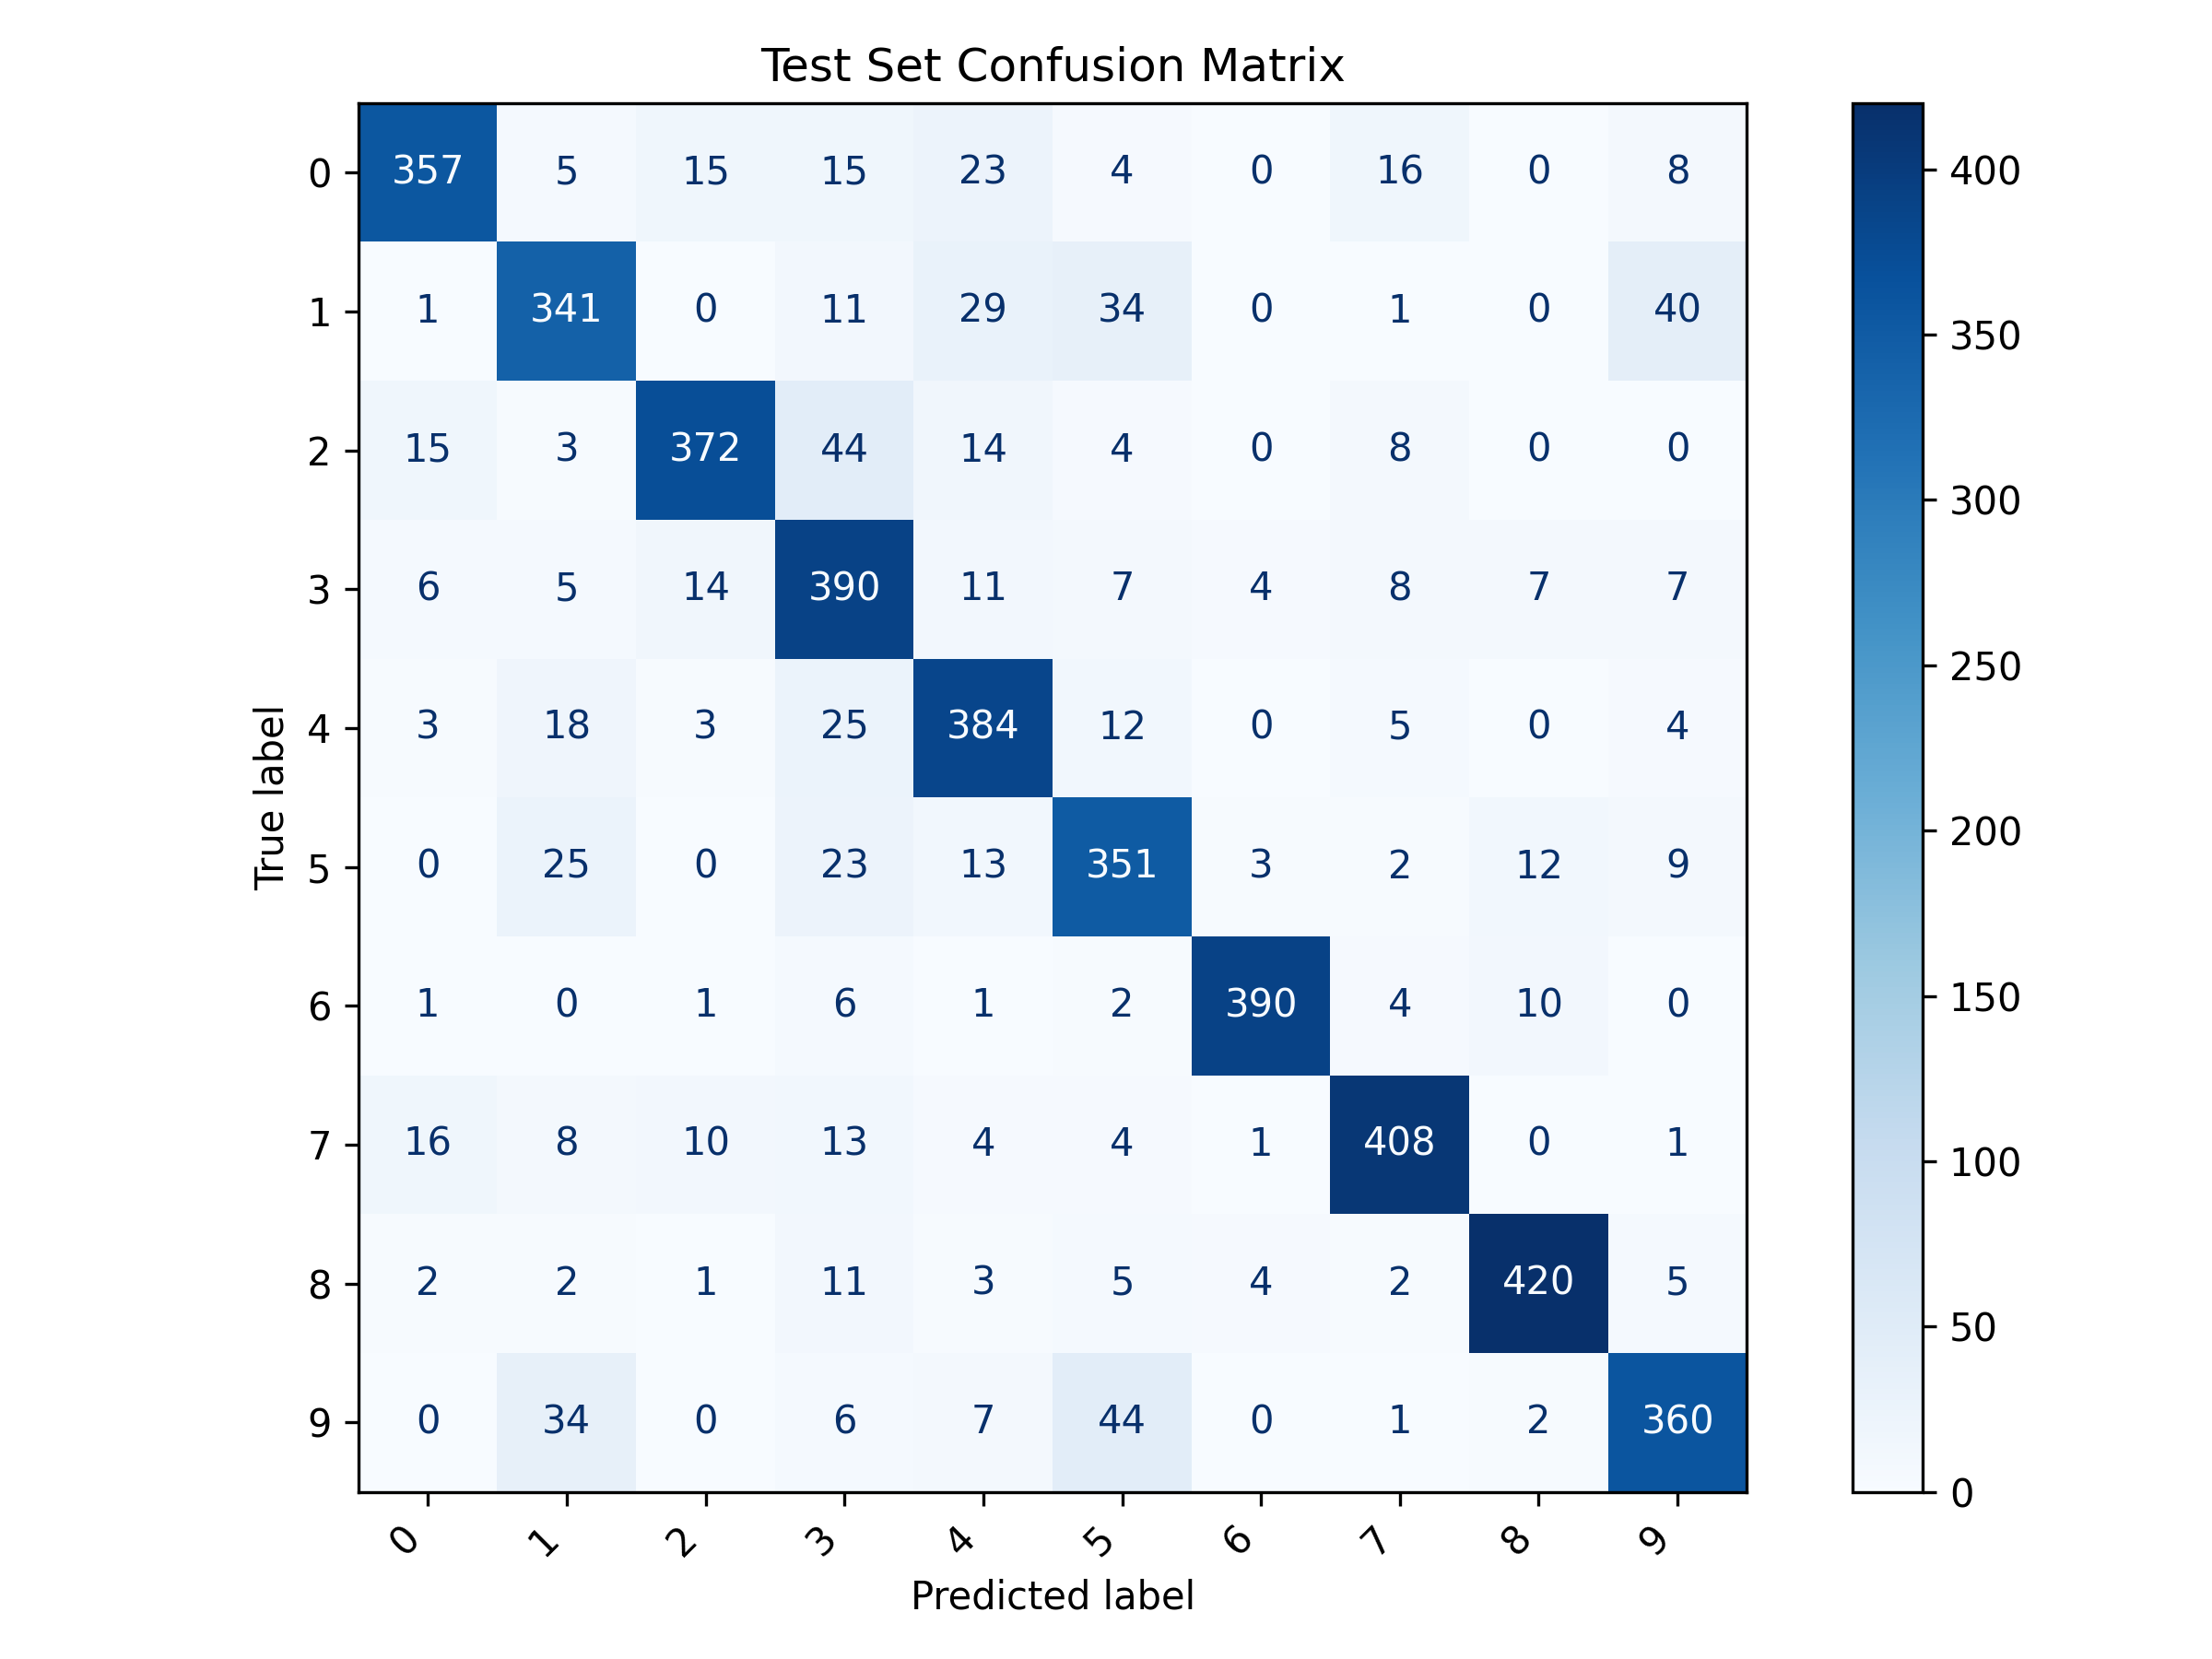
\includegraphics[width=0.95\linewidth]{graphics-bilateral-da/bilateral-da-confusion-matrix.png}
    \caption{Matriz de confusión del conjunto de prueba para Bilateral Filter with Data Augmentation.}
    \label{fig:bilateral-da-confusion-matrix}
\end{figure}
\noindent\textit{
La Figura~\ref{fig:bilateral-da-confusion-matrix} muestra la matriz de confusión obtenida en el conjunto de prueba. Se observa que, aunque la mayoría de las predicciones se concentran en la diagonal principal, existen confusiones notables entre algunas clases, especialmente la clase 1 y la clase 9. Estas confusiones sugieren que existen similitudes acústicas entre ciertos dígitos o posibles desbalances en el dataset.
}

\section{Conclusión Modelo A: LeNet-5}

El análisis exhaustivo de los resultados obtenidos con el Modelo A (LeNet-5) permite concluir que el mejor desempeño se alcanza utilizando el dataset \textit{Raw without Data Augmentation}. Este dataset, que consiste en los espectrogramas originales sin técnicas adicionales de aumento de datos ni filtrado, logra los valores más altos de accuracy, F1-score, precisión y recall en los conjuntos de prueba, validación y entrenamiento, superando consistentemente a las demás variantes evaluadas.

La superioridad del dataset \textit{Raw without Data Augmentation} puede atribuirse a la calidad y representatividad de los datos originales, que permiten al modelo aprender patrones discriminativos de manera eficiente sin la introducción de ruido o distorsión adicional. Si bien las técnicas de data augmentation, como el frequency masking, y los filtros bilaterales pueden ser útiles para mejorar la robustez en escenarios con menos datos o mayor variabilidad, en este caso particular, el dataset original ya proporciona suficiente diversidad y calidad para un aprendizaje efectivo.

En cuanto a los hiperparámetros, los mejores resultados se obtuvieron con un \textit{learning rate} de 0.0007 y 30 épocas de entrenamiento. Esta configuración permitió al modelo converger de manera estable, maximizando el desempeño sin incurrir en sobreajuste. El número de épocas fue suficiente para que el modelo aprovechara al máximo la información disponible, mientras que el learning rate facilitó una actualización eficiente de los pesos, evitando tanto la convergencia prematura como la oscilación en la función de pérdida.

El Modelo A demuestra que, para el problema de clasificación de dígitos en el dataset Audio MNIST, el uso de los datos originales sin modificaciones adicionales y un ajuste cuidadoso de los hiperparámetros es la estrategia más efectiva. Las modificaciones como data augmentation y filtrado bilateral, aunque útiles en otros contextos, no superan el rendimiento del dataset original en este caso, probablemente debido a la alta calidad y balance de los datos de entrada.

Para un análisis interactivo y visualización detallada de los experimentos, véase el Apéndice~\ref{appendix:wandb}.

\section{Modelo B: ResNet personalizado}

El Modelo B se basa en una arquitectura de tipo ResNet~\cite{resnet_original}, reconocida por su capacidad de aprendizaje profundo mediante el uso de conexiones residuales, lo que permite entrenar redes muy profundas sin sufrir el problema del desvanecimiento del gradiente. ResNet ha sido adaptada exitosamente a tareas de clasificación de audio~\cite{resnet_audio, resnet_audio2}, mostrando mejoras significativas en la generalización y robustez frente a variaciones en los datos. Para este proyecto, se utilizó una variante personalizada de ResNet-18, ajustada para trabajar con espectrogramas acústicos como entrada.

La arquitectura del modelo inicia con una capa convolucional adaptada a imágenes de un solo canal (convertidas a tres canales por replicación), seguida de capas residuales distribuidas en cuatro bloques con downsampling progresivo. Se aplicó un `dropout` antes de la capa totalmente conectada para reducir el sobreajuste. El entrenamiento se realizó utilizando el optimizador Adam y se exploraron distintos valores para el parámetro \textit{weight decay}, clave para controlar la magnitud de los pesos y prevenir el sobreajuste.

\subsection{Evaluación de weight decay}

Se probaron varios valores de \textit{weight decay} y se registraron los resultados en términos de métricas tanto de entrenamiento como de validación. El valor seleccionado final fue $1\mathrm{e}{-6}$, ya que ofreció un buen equilibrio entre precisión y generalización, logrando el mejor rendimiento en validación.

Este comportamiento en la tabla ~\ref{tab:weight-decay} refleja cómo un valor muy bajo (como $1\mathrm{e}{-7}$) permite un sobreajuste evidente, mientras que valores más altos (como $1\mathrm{e}{-4}$) pueden restringir demasiado la capacidad del modelo de aprender características relevantes. El valor óptimo de $1\mathrm{e}{-6}$ mantiene un buen balance entre pérdida de entrenamiento y validación.


\begin{table}[h]
    \centering
    \begin{tabular}{|c|c|c|c|c|c|c|}
        \hline
        \textbf{Weight D.} & \textbf{T. Acc.} & \textbf{V. Acc.} & \textbf{T. F1} & \textbf{V. F1} & \textbf{T. Loss} & \textbf{V. Loss} \\
        \hline
        1e-4 & 0.971 & 0.855 & 0.964 & 0.851 & 0.096 & 0.442 \\
        1e-5 & 0.976 & 0.869 & 0.970 & 0.859 & 0.087 & 0.434 \\
        1e-7 & 0.980 & 0.771 & 0.974 & 0.764 & 0.081 & 0.835 \\
        1e-6 & 0.975 & \textbf{0.919} & 0.968 & \textbf{0.911} & 0.093 & \textbf{0.271} \\
        \hline
    \end{tabular}
    \caption{Comparación de resultados para distintos valores de weight decay.}
    \label{tab:weight-decay}
\end{table}

\subsection{ResNet - Raw - Without Augmentation}

\begin{figure}[H]
    \centering
    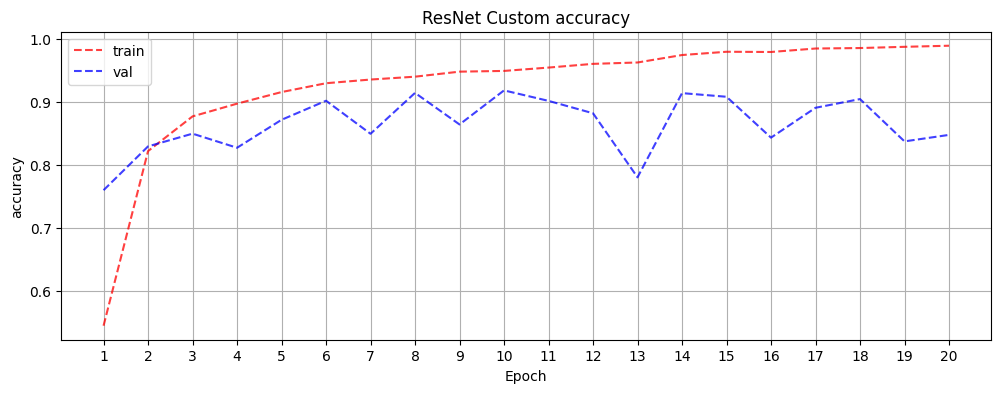
\includegraphics[width=0.95\linewidth]{graphics-resnet-raw/resnet_raw_without_accuracy.png}
    \caption{Accuracy por época para ResNet con datos sin procesar y sin aumentación.}
    \label{fig:resnet_raw_without_accuracy}
\end{figure}
\noindent\textit{%
La Figura~\ref{fig:resnet_raw_without_accuracy} muestra la evolución de la precisión (accuracy) durante el entrenamiento del modelo ResNet personalizado a lo largo de 20 épocas. Se observa una tendencia ascendente en el conjunto de entrenamiento, que parte de \(\approx0.55\) en la época 1 y supera \(\approx0.95\) a partir de la época 12, alcanzando casi 0.99 al finalizar. En el conjunto de validación, aunque al inicio mejora hasta \(\approx0.92\) en las primeras 8–9 épocas, la curva presenta oscilaciones posteriores (entre \(\approx0.78\) y \(\approx0.92\)) sin una mejora sostenida.
}

\begin{figure}[H]
    \centering
    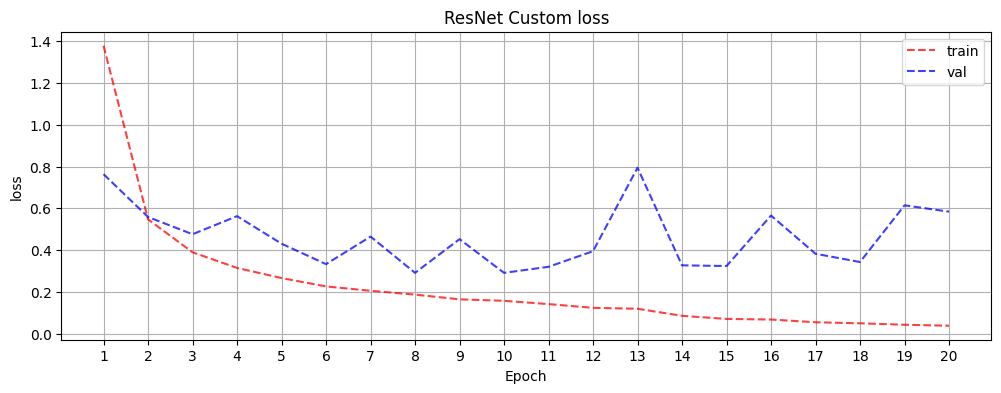
\includegraphics[width=0.95\linewidth]{graphics-resnet-raw/resnet_raw_without_loss.png}
    \caption{Pérdida por época para ResNet con datos sin procesar y sin aumentación.}
    \label{fig:resnet_raw_without_loss}
\end{figure}
\noindent\textit{%
La Figura~\ref{fig:resnet_raw_without_loss} muestra la evolución de la función de pérdida (loss) durante el entrenamiento del modelo ResNet con datos sin procesar y sin aumentación. Se observa que la pérdida de entrenamiento desciende de forma continua desde \(\approx1.40\) en la época 1 hasta valores próximos a cero al finalizar, lo cual indica un ajuste progresivo al conjunto de entrenamiento.
}

\begin{figure}[H]
    \centering
    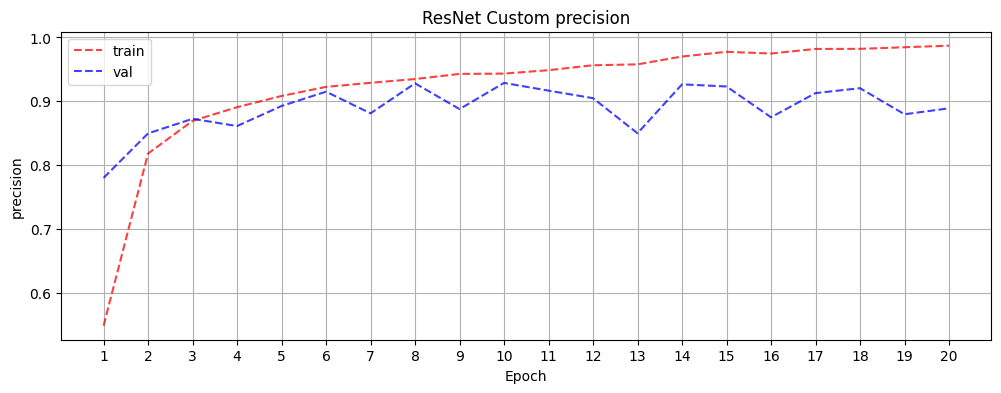
\includegraphics[width=0.95\linewidth]{graphics-resnet-raw/resnet_raw_without_precision.png}
    \caption{Precisión por época para ResNet con datos sin procesar y sin aumentación.}
    \label{fig:resnet_raw_without_precision}
\end{figure}
\noindent\textit{%
La Figura~\ref{fig:resnet_raw_without_precision} muestra la evolución de la precisión (precision) durante el entrenamiento del modelo ResNet con datos sin procesar y sin aumentación a lo largo de 20 épocas. Se aprecia que la precisión de entrenamiento aumenta de forma constante desde \(\approx0.55\) en la época 1 hasta casi \(\approx0.99\) al finalizar, demostrando un ajuste progresivo al conjunto de entrenamiento. En el conjunto de validación, la precisión sube inicialmente hasta \(\approx0.92\) en las primeras 8–9 épocas, pero luego presenta fluctuaciones (por ejemplo, una caída a \(\approx0.87\) en la época 13 y un nuevo pico en torno a \(\approx0.93\) en la época 15) sin tendencia ascendente sostenida.
}

\begin{figure}[H]
    \centering
    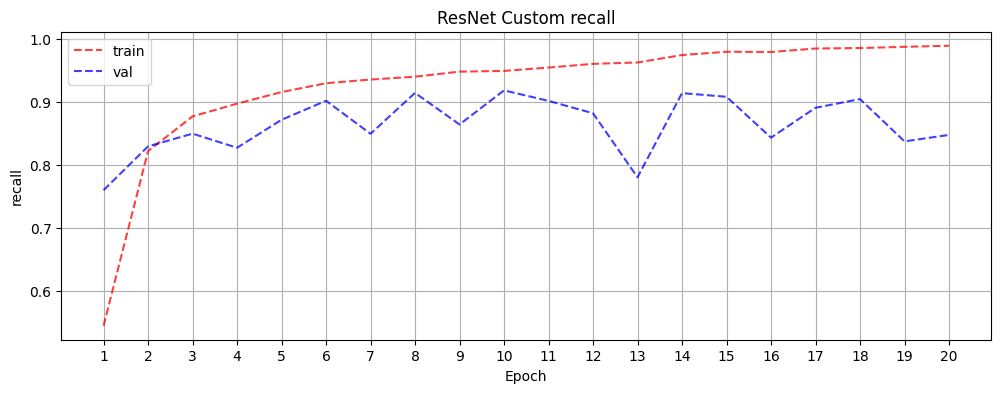
\includegraphics[width=0.95\linewidth]{graphics-resnet-raw/resnet_raw_without_recall.png}
    \caption{Recall por época para ResNet con datos sin procesar y sin aumentación.}
    \label{fig:resnet_raw_without_recall}
\end{figure}
\noindent\textit{%
La Figura~\ref{fig:resnet_raw_without_recall} muestra la evolución del recall (recall) durante el entrenamiento del modelo ResNet con datos sin procesar y sin aumentación a lo largo de 20 épocas. Se observa que el recall de entrenamiento aumenta de forma constante desde \(\approx0.55\) en la época 1 hasta casi \(\approx0.99\) al finalizar, indicando un ajuste progresivo al conjunto de entrenamiento. En el conjunto de validación, el recall mejora inicialmente hasta \(\approx0.92\) en las primeras 8–10 épocas, pero a partir de ahí presenta fluctuaciones (por ejemplo, una caída a \(\approx0.78\) en la época 13 y un pico cercano a \(\approx0.91\) en la época 15) sin una tendencia ascendente sostenida.
}

\begin{figure}[H]
    \centering
    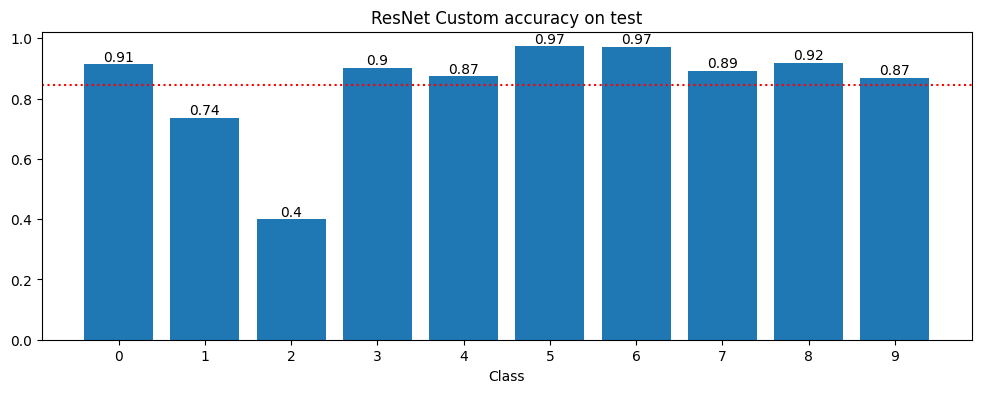
\includegraphics[width=0.45\textwidth]{graphics-resnet-raw/resnet_raw_without_class_accuracy.png}
    \caption{Accuracy por clase en el conjunto de prueba.}
    \label{fig:resnet_raw_without_class_accuracy}
\end{figure}
\noindent\textit{%
La Figura~\ref{fig:resnet_raw_without_class_accuracy} muestra la precisión obtenida por cada clase en el conjunto de prueba. Se observa que las clases 5 y 6 alcanzan el mejor desempeño con una precisión de \(\approx0.97\), mientras que la clase 2 presenta el valor más bajo (\(\approx0.40\)) y la clase 1 queda en \(\approx0.74\). La línea punteada horizontal indica la precisión promedio global (\(\approx0.85\)). 
}

\begin{figure}[H]
    \centering
    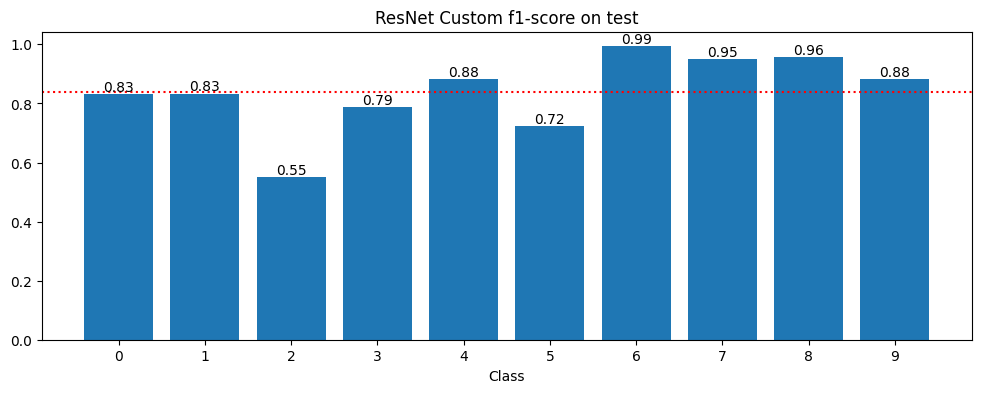
\includegraphics[width=0.45\textwidth]{graphics-resnet-raw/resnet_raw_without_class_f1.png}
    \caption{F1-score por clase en el conjunto de prueba.}
    \label{fig:resnet_raw_without_class_f1}
\end{figure}
\noindent\textit{%
La Figura~\ref{fig:resnet_raw_without_class_f1} muestra el F1-score obtenido por cada clase en el conjunto de prueba. Se observa un rendimiento excepcional en las clases 6, 7 y 8, con valores de \(\approx0.99\), \(\approx0.95\) y \(\approx0.96\) respectivamente, mientras que la clase 2 presenta el valor más bajo (\(\approx0.55\)). Las clases 0, 1, 4 y 9 se sitúan en torno a \(\approx0.88\)–\(\approx0.93\), y la clase 5 arroja un F1 moderado (\(\approx0.72\)). La línea punteada horizontal indica el F1 promedio global (\(\approx0.86\)).
}

\begin{figure}[H]
    \centering
    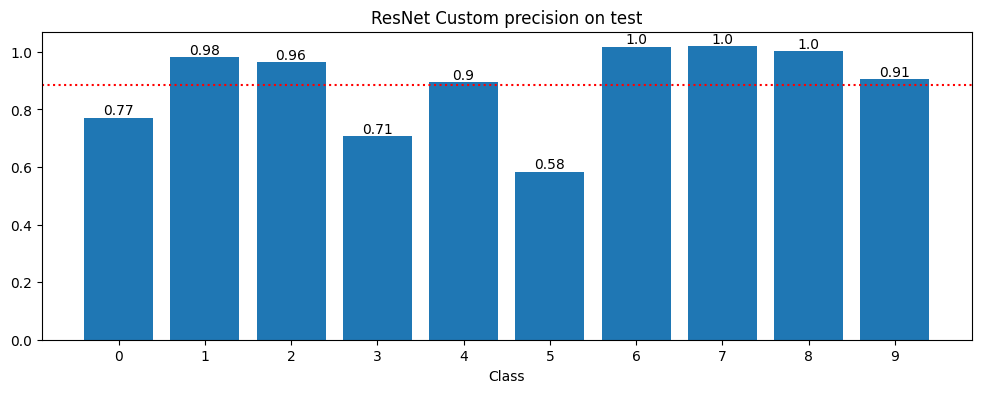
\includegraphics[width=0.45\textwidth]{graphics-resnet-raw/resnet_raw_without_class_precision.png}
    \caption{Precisión por clase en el conjunto de prueba.}
    \label{fig:resnet_raw_without_class_precision}
\end{figure}
\noindent\textit{%
La Figura~\ref{fig:resnet_raw_without_class_precision} muestra la precisión obtenida por cada clase en el conjunto de prueba. Se observa que las clases 6, 7 y 8 alcanzan un desempeño perfecto (\(1.00\)), mientras que las clases 1 y 2 presentan valores muy altos (\(\approx0.98\) y \(\approx0.96\), respectivamente). La clase 4 y la clase 9 también se sitúan por encima de la media global (\(\approx0.90\) y \(\approx0.91\)). En contraste, la clase 0 muestra una precisión moderada (\(\approx0.77\)), la clase 3 baja a \(\approx0.71\) y la clase 5 obtiene el valor más bajo (\(\approx0.58\)). La línea punteada horizontal indica la precisión promedio global (\(\approx0.85\)).
}

\begin{figure}[H]
    \centering
    \includegraphics[width=0.45\textwidth]{graphics-resnet-raw/resnet_raw_without_confusion_matrix.png}
    \caption{Matriz de confusión.}
    \label{fig:resnet_raw_without_confusion_matrix}
\end{figure}
\noindent\textit{%
La Figura~\ref{fig:resnet_raw_without_confusion_matrix} muestra la matriz de confusión obtenida en el conjunto de prueba. Se observa que la mayoría de las predicciones se concentran en la diagonal principal con recuentos altos (por ejemplo, 453 para la clase 3, 449 para la clase 6 y 464 para la clase 9), lo que indica un buen desempeño global. Sin embargo, existen confusiones relevantes: la clase 1 se confunde 45 veces con la clase 9, la clase 2 presenta 43 ejemplos erróneos y la clase 5 se etiqueta erróneamente como 1 en 15 ocasiones. Otras clases como la 4 y la 7 tienen pequeños volúmenes de error alrededor de 10 y 7 casos respectivamente. Estas desviaciones sugieren la necesidad de técnicas de reequilibrio o aumento de datos focalizado para reducir los errores en las clases más confundidas y mejorar la robustez del modelo.%
}

\begin{table}[H]
    \centering
    \begin{tabular}{|c|c|}
        \hline
        \textbf{Hiperparámetro} & \textbf{Valor} \\
        \hline
        Arquitectura & ResNet Custom \\
        Learning Rate & 0.0001 \\
        Epochs & 10 \\
        Optimizer & Adam \\
        Weight Decay & 1e-6 \\
        Batch Size & 118 \\
        Aumentación & No \\
        \hline
    \end{tabular}
    \caption{Hiperparámetros utilizados en el entrenamiento.}
    \label{tab:resnet_raw_without_hparams}
\end{table}
\noindent\textit{%
La Tabla~\ref{tab:resnet_raw_without_hparams} presenta los valores de hiperparámetros empleados para entrenar la versión sin procesar y sin aumentación del modelo ResNet. Se utilizó un learning rate bajo (0.0001) junto con Adam y un weight decay mínimo (1e-6) para controlar la actualización de pesos y evitar cambios bruscos. El entrenamiento se limitó a 10 épocas con un batch size de 118, lo cual acelera el proceso pero puede resultar insuficiente para una convergencia óptima. La ausencia de aumentación de datos hace más probable el sobreajuste.
}

\subsection{ResNet - Raw - With Augmentation}

\begin{figure}[H]
    \centering
    \includegraphics[width=0.45\textwidth]{graphics-resnet-raw/resnet_raw_with_accuracy.png}
    \caption{Accuracy por época para ResNet con datos sin procesar y con aumentación.}
    \label{fig:resnet_raw_with_accuracy}
\end{figure}
\noindent\textit{%
La Figura~\ref{fig:resnet_raw_with_accuracy} muestra la evolución de la precisión (accuracy) durante el entrenamiento del modelo ResNet con datos sin procesar y con aumentación a lo largo de 10 épocas. Se observa una tendencia ascendente en ambos conjuntos: la precisión de entrenamiento aumenta de \(\approx0.55\) en la época 1 a \(\approx0.96\) en la época 10, mientras que la precisión de validación mejora de \(\approx0.78\) a \(\approx0.94\). La proximidad constante entre ambas curvas a partir de la época 3 indica una adecuada generalización y sugiere que el uso de aumentación ha reducido el sobreajuste, validando la elección de los hiperparámetros para este escenario.%
}

\begin{figure}[H]
    \centering
    \includegraphics[width=0.45\textwidth]{graphics-resnet-raw/resnet_raw_with_loss.png}
    \caption{Pérdida por época para ResNet con datos sin procesar y con aumentación.}
    \label{fig:resnet_raw_with_loss}
\end{figure}
\noindent\textit{%
La Figura~\ref{fig:resnet_raw_with_loss} muestra la evolución de la función de pérdida (loss) durante el entrenamiento del modelo ResNet con datos sin procesar y con aumentación a lo largo de 10 épocas. Se observa un descenso pronunciado en la pérdida de entrenamiento desde \(\approx1.40\) en la época 1 hasta \(\approx0.12\) en la época 10, indicando un ajuste continuo al conjunto de entrenamiento. La pérdida de validación sigue de cerca la de entrenamiento, bajando de \(\approx0.80\) a \(\approx0.20\) en las primeras 4 épocas, con ligeras oscilaciones posteriores (por ejemplo, \(\approx0.35\) en la época 7 y \(\approx0.18\) en la época 10). La cercanía de ambas curvas y la reducción de sus fluctuaciones sugieren que la aumentación de datos ha mejorado la capacidad de generalización del modelo.%
}

\begin{figure}[H]
    \centering
    \includegraphics[width=0.95\linewidth]{graphics-resnet-raw/resnet_raw_with_precision.png}
    \caption{Precisión por época para ResNet con datos sin procesar y con aumentación.}
    \label{fig:resnet_raw_with_precision}
\end{figure}
\noindent\textit{%
La Figura~\ref{fig:resnet_raw_with_precision} muestra la evolución de la precisión (precision) durante el entrenamiento del modelo ResNet con datos sin procesar y con aumentación a lo largo de 10 épocas. Se aprecia que la precisión de validación supera la de entrenamiento en las primeras épocas (por ejemplo, \(\approx0.83\) frente a \(\approx0.78\) en la época 2), lo que indica una mayor robustez inicial gracias a la aumentación. A partir de la época 4 ambas curvas convergen alrededor de \(\approx0.92\)–\(\approx0.95\), y al finalizar alcanzan valores cercanos a \(\approx0.95\) (entrenamiento) y \(\approx0.94\) (validación). La estrecha proximidad sostenida entre ambas curvas evidencia una buena capacidad de generalización y una efectiva reducción del sobreajuste.%
}

\begin{figure}[H]
    \centering
    \includegraphics[width=0.45\textwidth]{graphics-resnet-raw/resnet_raw_with_recall.png}
    \caption{Recall por época para ResNet con datos sin procesar y con aumentación.}
    \label{fig:resnet_raw_with_recall}
\end{figure}
\noindent\textit{%
La Figura~\ref{fig:resnet_raw_with_recall} muestra la evolución del recall durante el entrenamiento del modelo ResNet con datos sin procesar y con aumentación a lo largo de 10 épocas. El recall de entrenamiento parte de \(\approx0.52\) en la época 1, experimenta un salto hasta \(\approx0.82\) en la época 2 y alcanza casi \(\approx0.96\) al finalizar, lo que evidencia un aprendizaje progresivo. En el conjunto de validación, el recall mejora de \(\approx0.75\) a \(\approx0.92\) en las primeras 5 épocas, con ligeras oscilaciones posteriores (por ejemplo, una caída a \(\approx0.89\) en la época 7 y un pico de \(\approx0.95\) en la época 9). La estrecha proximidad entre ambas curvas tras la época 3 sugiere que la aumentación de datos ha contribuido a estabilizar la generalización y mitigar el sobreajuste.%
}

\begin{figure}[H]
    \centering
    \includegraphics[width=0.45\textwidth]{graphics-resnet-raw/resnet_raw_with_class_accuracy.png}
    \caption{Accuracy por clase en el conjunto de prueba.}
    \label{fig:resnet_raw_with_class_accuracy}
\end{figure}
\noindent\textit{%
La Figura~\ref{fig:resnet_raw_with_class_accuracy} muestra la precisión obtenida por cada clase en el conjunto de prueba tras aplicar aumentación. La clase 4 alcanza un rendimiento perfecto (\(\approx1.00\)), mientras que las clases 0, 2, 5, 7 y 8 obtienen puntuaciones altas (\(\approx0.95\)). Por contraste, la clase 1 presenta la precisión más baja (\(\approx0.85\)), seguida por la clase 3 (\(\approx0.84\)) y la clase 9 (\(\approx0.88\)). La línea punteada horizontal indica la precisión global promedio (\(\approx0.92\)). 
}

\begin{figure}[H]
    \centering
    \includegraphics[width=0.45\textwidth]{graphics-resnet-raw/resnet_raw_with_class_f1.png}
    \caption{F1-score por clase en el conjunto de prueba.}
    \label{fig:resnet_raw_with_class_f1}
\end{figure}
\noindent\textit{%
La Figura~\ref{fig:resnet_raw_with_class_f1} muestra el F1-score obtenido por cada clase en el conjunto de prueba tras aplicar aumentación. Se aprecia que la clase 6 alcanza un valor perfecto (\(\approx1.00\)), seguida de la clase 7 (\(\approx0.98\)) y la clase 0 (\(\approx0.96\)). Las clases 1 y 9 presentan valores robustos (\(\approx0.91\) y \(\approx0.92\) respectivamente), mientras que las clases 3, 4 y 5 quedan en torno a \(\approx0.89\). La línea punteada horizontal indica el F1-score promedio global (\(\approx0.93\)).
}

\begin{figure}[H]
    \centering
    \includegraphics[width=0.45\textwidth]{graphics-resnet-raw/resnet_raw_with_class_precision.png}
    \caption{Precisión por clase en el conjunto de prueba.}
    \label{fig:resnet_raw_with_class_precision}
\end{figure}
\noindent\textit{%
La Figura~\ref{fig:resnet_raw_with_class_precision} muestra la precisión obtenida por cada clase en el conjunto de prueba tras aplicar aumentación. Se aprecia un desempeño perfecto en las clases 6 y 7 (\(\approx1.00\)), y muy alto en las clases 0, 1, 3, 8 y 9 (entre \(\approx0.96\) y \(\approx0.99\)). Por contraste, las clases 2 y 4 presentan los valores más bajos (\(\approx0.86\) y \(\approx0.81\), respectivamente), seguidas de cerca por la clase 5 (\(\approx0.85\)). La línea punteada horizontal indica la precisión global promedio (\(\approx0.93\)). 
}

\begin{figure}[H]
    \centering
    \includegraphics[width=0.45\textwidth]{graphics-resnet-raw/resnet_raw_with_confusion_matrix.png}
    \caption{Matriz de confusión.}
    \label{fig:resnet_raw_with_confusion_matrix}
\end{figure}
\noindent\textit{%
La Figura~\ref{fig:resnet_raw_with_confusion_matrix} muestra la matriz de confusión obtenida en el conjunto de prueba tras aplicar aumentación. Se observa un alto número de aciertos en la diagonal principal (por ejemplo, 442 para la clase 4, 414 para la clase 6 y 398 para la clase 7), lo que refleja un buen desempeño global. Sin embargo, existen confusiones relevantes: la clase 3 se confunde en 90 ocasiones como 1 y en 39 como 2; la clase 5 es erróneamente etiquetada 61 veces como 1 y 31 como 4; la clase 8 presenta 28 confusiones con la clase 1 y 15 con la clase 2; y la clase 9 se etiqueta 49 veces como 1. También se aprecian ventanas de error en la clase 0 (14 como 1 y 15 como 4). Estas desviaciones sugieren la necesidad de focalizar futuras estrategias de reequilibrio de clases o aumentación dirigida para reducir los errores en las clases más confundidas y mejorar la robustez del modelo.%
}

\begin{table}[H]
    \centering
    \begin{tabular}{|c|c|}
        \hline
        \textbf{Hiperparámetro} & \textbf{Valor} \\
        \hline
        Arquitectura    & ResNet Custom \\
        Learning Rate   & 0.0001        \\
        Epochs          & 10            \\
        Optimizer       & Adam          \\
        Weight Decay    & 1e-6          \\
        Batch Size      & 118           \\
        Aumentación     & Sí (Frequency + Time Masking) \\
        \hline
    \end{tabular}
    \caption{Hiperparámetros utilizados en el entrenamiento.}
    \label{tab:resnet_raw_with_hparams}
\end{table}
\noindent\textit{%
La Tabla~\ref{tab:resnet_raw_with_hparams} presenta los hiperparámetros empleados para entrenar la versión con aumentación del modelo ResNet. Se mantiene un learning rate bajo (0.0001) junto con Adam y un weight decay de 1e-6 para estabilizar las actualizaciones de pesos. El entrenamiento se configura en 10 épocas con un batch size de 118. La inclusión de aumentación mediante Frequency y Time Masking contribuye a incrementar la variabilidad del conjunto de entrenamiento, lo que ayuda a mejorar la generalización sin necesidad de ampliar el número de épocas.
}

\subsection{ResNet - Bilateral - Without Augmentation}

\begin{figure}[H]
    \centering
    \includegraphics[width=0.45\textwidth]{graphics-resnet-bilateral/resnet_bilateral_without_accuracy.png}
    \caption{Accuracy por época para ResNet con filtro bilateral y sin aumentación.}
    \label{fig:resnet_bilateral_without_accuracy}
\end{figure}
\noindent\textit{%
La Figura~\ref{fig:resnet_bilateral_without_accuracy} muestra la evolución de la precisión (accuracy) durante el entrenamiento del modelo ResNet aplicado tras filtro bilateral, sin aumentación, a lo largo de 20 épocas. Se observa que la precisión de entrenamiento parte de \(\approx0.55\) en la época 1, supera \(\approx0.90\) a partir de la época 4 y alcanza casi \(\approx0.99\) al finalizar, lo que indica un ajuste muy progresivo al conjunto de entrenamiento. En el conjunto de validación, la precisión asciende inicialmente de \(\approx0.75\) a \(\approx0.92\) en las primeras 8–9 épocas, pero a continuación presenta oscilaciones entre \(\approx0.78\) y \(\approx0.92\) sin tendencia ascendente clara. 
}

\begin{figure}[H]
    \centering
    \includegraphics[width=0.45\textwidth]{graphics-resnet-bilateral/resnet_bilateral_without_loss.png}
    \caption{Pérdida por época para ResNet con filtro bilateral y sin aumentación.}
    \label{fig:resnet_bilateral_without_loss}
\end{figure}
\noindent\textit{%
La Figura~\ref{fig:resnet_bilateral_without_loss} muestra la evolución de la función de pérdida (loss) durante el entrenamiento del modelo ResNet tras aplicar filtro bilateral, sin técnicas de aumentación, a lo largo de 20 épocas. La pérdida de entrenamiento desciende de forma constante desde \(\approx1.40\) en la época 1 hasta valores mínimos cercanos a \(\approx0.05\) en la época 20, lo que refleja un ajuste continuo al conjunto de entrenamiento. Por su parte, la pérdida de validación baja inicialmente hasta \(\approx0.60\) en la época 2, pero a partir de la época 3 presenta oscilaciones (por ejemplo, picos de \(\approx0.55\) en la época 4 y \(\approx0.80\) en la época 13, y mínimos de \(\approx0.30\) en la época 15), sin una tendencia sostenida de descenso.
}

\begin{figure}[H]
    \centering
    \includegraphics[width=0.45\textwidth]{graphics-resnet-bilateral/resnet_bilateral_without_precision.png}
    \caption{Precisión por época para ResNet con filtro bilateral y sin aumentación.}
    \label{fig:resnet_bilateral_without_precision}
\end{figure}
\noindent\textit{%
La Figura~\ref{fig:resnet_bilateral_without_precision} muestra la evolución de la precisión (precision) durante el entrenamiento del modelo ResNet tras aplicar filtro bilateral sin técnicas de aumentación a lo largo de 20 épocas. Se observa un incremento constante de la precisión de entrenamiento desde \(\approx0.55\) en la época 1 hasta \(\approx0.99\) en la época 20. En el conjunto de validación, la precisión sube hasta \(\approx0.93\) alrededor de las épocas 8–9, pero a partir de ahí oscila entre \(\approx0.85\) y \(\approx0.93\) sin un ascenso sostenido.
}

\begin{figure}[H]
    \centering
    \includegraphics[width=0.45\textwidth]{graphics-resnet-bilateral/resnet_bilateral_without_recall.png}
    \caption{Recall por época para ResNet con filtro bilateral y sin aumentación.}
    \label{fig:resnet_bilateral_without_recall}
\end{figure}
\noindent\textit{%
La Figura~\ref{fig:resnet_bilateral_without_recall} muestra la evolución del recall durante el entrenamiento del modelo ResNet tras aplicar filtro bilateral, sin técnicas de aumentación, a lo largo de 20 épocas. El recall de entrenamiento parte de \(\approx0.55\) en la época 1, alcanza \(\approx0.82\) en la época 2 y progresa hasta casi \(\approx0.99\) al finalizar, evidenciando un aprendizaje firme sobre el conjunto de entrenamiento. En el conjunto de validación, el recall mejora de \(\approx0.75\) a \(\approx0.90\) durante las primeras 6–9 épocas, presenta una caída puntual a \(\approx0.78\) en la época 13 y un nuevo pico de \(\approx0.91\) en la época 15, para terminar alrededor de \(\approx0.84\).
}

\begin{figure}[H]
    \centering
    \includegraphics[width=0.45\textwidth]{graphics-resnet-bilateral/resnet_bilateral_without_class_accuracy.png}
    \caption{Accuracy por clase en el conjunto de prueba.}
    \label{fig:resnet_bilateral_without_class_accuracy}
\end{figure}
\noindent\textit{%
La Figura~\ref{fig:resnet_bilateral_without_class_accuracy} muestra la precisión obtenida por cada clase en el conjunto de prueba. Destacan las clases 5 y 6 con valores de \(\approx0.97\), así como varias categorías (0, 3, 4, 7, 8 y 9) que superan la precisión global indicada (\(\approx0.85\)).
}

\begin{figure}[H]
    \centering
    \includegraphics[width=0.45\textwidth]{graphics-resnet-bilateral/resnet_bilateral_without_class_f1.png}
    \caption{F1-score por clase en el conjunto de prueba.}
    \label{fig:resnet_bilateral_without_class_f1}
\end{figure}
\noindent\textit{%
La Figura~\ref{fig:resnet_bilateral_without_class_f1} muestra el F1-score obtenido por cada clase en el conjunto de prueba. Se aprecia que la mayoría de las clases supera el valor medio indicado (\(\approx0.83\)), destacando especialmente las clases 6 (\(\approx0.99\)), 7 (\(\approx0.95\)) y 8 (\(\approx0.96\)). Además, las clases 4 y 9 alcanzan valores de \(\approx0.88\), mientras que las clases 0 y 1 se sitúan en el promedio con \(\approx0.83\). Estos resultados reflejan un desempeño equilibrado y consistente en el conjunto de prueba.%
}


\begin{figure}[H]
    \centering
    \includegraphics[width=0.45\textwidth]{graphics-resnet-bilateral/resnet_bilateral_without_class_f1.png}
    \caption{F1-score por clase en el conjunto de prueba.}
    \label{fig:resnet_bilateral_without_class_f1}
\end{figure}
\noindent\textit{%
La Figura~\ref{fig:resnet_bilateral_without_class_f1} muestra el F1-score obtenido por cada clase en el conjunto de prueba. Se aprecia que la mayoría de las clases supera el valor medio indicado (\(\approx0.83\)), destacando especialmente las clases 6 (\(\approx0.99\)), 7 (\(\approx0.95\)) y 8 (\(\approx0.96\)). Además, las clases 4 y 9 alcanzan valores de \(\approx0.88\), mientras que las clases 0 y 1 se sitúan en el promedio con \(\approx0.83\). Estos resultados reflejan un desempeño equilibrado y consistente en el conjunto de prueba.%
}

\begin{table}[H]
    \centering
    \begin{tabular}{|c|c|}
        \hline
        \textbf{Hiperparámetro} & \textbf{Valor} \\
        \hline
        Arquitectura       & ResNet Custom \\
        Learning Rate      & 0.0001        \\
        Epochs             & 10            \\
        Optimizer          & Adam          \\
        Weight Decay       & 1e-6          \\
        Batch Size         & 118           \\
        Filtro Bilateral   & Sí            \\
        Aumentación        & No            \\
        \hline
    \end{tabular}
    \caption{Hiperparámetros utilizados en el entrenamiento.}
    \label{tab:resnet_bilateral_without_hparams}
\end{table}
\noindent\textit{%
La Tabla~\ref{tab:resnet_bilateral_without_hparams} presenta los hiperparámetros empleados para el entrenamiento del modelo ResNet con filtro bilateral y sin aumentación. La combinación de un learning rate bajo (0.0001) con Adam y un weight decay de 1e-6, junto a un batch size de 118 en 10 épocas, asegura un proceso de optimización estable y preciso, mientras que el filtro bilateral contribuye a realzar las características relevantes de los datos.%
}

\subsection{ResNet - Bilateral - With Augmentation}

\begin{figure}[H]
    \centering
    \includegraphics[width=0.45\textwidth]{graphics-resnet-bilateral/resnet_bilateral_with_accuracy.png}
    \caption{Accuracy por época para ResNet con filtro bilateral y con aumentación.}
    \label{fig:resnet_bilateral_with_accuracy}
\end{figure}
\noindent\textit{%
La Figura~\ref{fig:resnet_bilateral_with_accuracy} muestra la evolución de la precisión (accuracy) durante el entrenamiento del modelo ResNet con filtro bilateral y aplicando aumentación a lo largo de 10 épocas. Se aprecia un crecimiento continuo desde \(\approx0.53\) (entrenamiento) y \(\approx0.75\) (validación) en la época 1, hasta alcanzar \(\approx0.94\) y \(\approx0.93\) respectivamente en la época 10. La estrecha proximidad entre ambas curvas desde la tercera época refleja una excelente capacidad de generalización y estabilidad a lo largo de todo el entrenamiento.%
}

\begin{figure}[H]
    \centering
    \includegraphics[width=0.45\textwidth]{graphics-resnet-bilateral/resnet_bilateral_with_loss.png}
    \caption{Pérdida por época para ResNet con filtro bilateral y con aumentación.}
    \label{fig:resnet_bilateral_with_loss}
\end{figure}
\noindent\textit{%
La Figura~\ref{fig:resnet_bilateral_with_loss} muestra la evolución de la función de pérdida (loss) durante el entrenamiento del modelo ResNet con filtro bilateral y aplicando aumentación a lo largo de 10 épocas. Se observa una disminución continua de la pérdida de entrenamiento desde \(\approx1.40\) en la época 1 hasta \(\approx0.15\) en la época 10, acompañada por una reducción de la pérdida de validación de \(\approx0.80\) a \(\approx0.25\).
}

\begin{figure}[H]
    \centering
    \includegraphics[width=0.45\textwidth]{graphics-resnet-bilateral/resnet_bilateral_with_precision.png}
    \caption{Precisión por época para ResNet con filtro bilateral y con aumentación.}
    \label{fig:resnet_bilateral_with_precision}
\end{figure}
\noindent\textit{%
La Figura~\ref{fig:resnet_bilateral_with_precision} muestra la evolución de la precisión durante el entrenamiento del modelo ResNet con filtro bilateral y aumentación a lo largo de 10 épocas. Se observa un rápido incremento en las primeras épocas, superando el \(\approx0.85\) desde la época 3, y alcanzando valores cercanos al \(\approx0.95\) en las últimas épocas.%
}

\begin{figure}[H]
    \centering
    \includegraphics[width=0.45\textwidth]{graphics-resnet-bilateral/resnet_bilateral_with_recall.png}
    \caption{Recall por época para ResNet con filtro bilateral y con aumentación.}
    \label{fig:resnet_bilateral_with_recall}
\end{figure}
\noindent\textit{%
La Figura~\ref{fig:resnet_bilateral_with_recall} muestra la evolución del recall durante el entrenamiento del modelo ResNet con filtro bilateral y con aumentación a lo largo de 10 épocas. El recall de entrenamiento parte de \(\approx0.53\) en la época 1, pasa a \(\approx0.82\) en la 2, \(\approx0.88\) en la 3, \(\approx0.90\) en la 4, \(\approx0.91\) en la 5, \(\approx0.92\) en la 6, \(\approx0.97\) en la 7, \(\approx0.98\) en la 8, \(\approx0.95\) en la 9 y \(\approx0.94\) en la 10. El recall de validación parte de \(\approx0.75\) en la época 1, alcanza \(\approx0.85\) en la 2, \(\approx0.87\) en la 3, \(\approx0.90\) en la 4, \(\approx0.89\) en la 5, \(\approx0.91\) en la 6, \(\approx0.89\) en la 7, \(\approx0.93\) en la 8, \(\approx0.95\) en la 9 y \(\approx0.94\) en la 10.%
}

\begin{figure}[H]
    \centering
    \includegraphics[width=0.45\textwidth]{graphics-resnet-bilateral/resnet_bilateral_with_class_f1.png}
    \caption{F1-score por clase en el conjunto de prueba.}
    \label{fig:resnet_bilateral_with_class_f1}
\end{figure}
\noindent\textit{%
La Figura~\ref{fig:resnet_bilateral_with_class_f1} muestra el F1-score por clase en el conjunto de prueba: clase 0 \(\approx0.96\), clase 1 \(\approx0.91\), clase 2 \(\approx0.90\), clase 3 \(\approx0.89\), clase 4 \(\approx0.89\), clase 5 \(\approx0.89\), clase 6 \(\approx1.00\), clase 7 \(\approx0.98\), clase 8 \(\approx0.95\) y clase 9 \(\approx0.92\). Estos resultados reflejan un desempeño equilibrado y sólido del modelo en el conjunto de prueba.%
}

\begin{figure}[H]
    \centering
    \includegraphics[width=0.45\textwidth]{graphics-resnet-bilateral/resnet_bilateral_with_class_f1.png}
    \caption{F1-score por clase en el conjunto de prueba.}
    \label{fig:resnet_bilateral_with_class_f1}
\end{figure}
\noindent\textit{%
La Figura~\ref{fig:resnet_bilateral_with_class_f1} muestra el F1-score obtenido por cada clase en el conjunto de prueba tras aplicar filtro bilateral y aumentación: clase 0 \(\approx0.96\), clase 1 \(\approx0.91\), clase 2 \(\approx0.90\), clase 3 \(\approx0.89\), clase 4 \(\approx0.89\), clase 5 \(\approx0.89\), clase 6 \(\approx1.00\), clase 7 \(\approx0.98\), clase 8 \(\approx0.95\) y clase 9 \(\approx0.92\). Estos valores confirman un desempeño robusto y consistente del modelo en todas las categorías.%
}

\begin{figure}[H]
    \centering
    \includegraphics[width=0.45\textwidth]{graphics-resnet-bilateral/resnet_bilateral_with_class_precision.png}
    \caption{Precisión por clase en el conjunto de prueba.}
    \label{fig:resnet_bilateral_with_class_precision}
\end{figure}
\noindent\textit{%
La Figura~\ref{fig:resnet_bilateral_with_class_precision} muestra la precisión por clase en el conjunto de prueba: clase 0 \(\approx0.98\), clase 1 \(\approx0.99\), clase 2 \(\approx0.86\), clase 3 \(\approx0.96\), clase 4 \(\approx0.81\), clase 5 \(\approx0.85\), clase 6 \(\approx1.00\), clase 7 \(\approx1.00\), clase 8 \(\approx0.96\) y clase 9 \(\approx0.98\). Estos valores confirman un desempeño robusto y consistente del modelo en todas las categorías.%
}

\begin{figure}[H]
    \centering
    \includegraphics[width=0.45\textwidth]{graphics-resnet-bilateral/resnet_bilateral_with_confusion_matrix.png}
    \caption{Matriz de confusión.}
    \label{fig:resnet_bilateral_with_confusion_matrix}
\end{figure}
\noindent\textit{%
La Figura~\ref{fig:resnet_bilateral_with_confusion_matrix} muestra la matriz de confusión con los siguientes recuentos por fila (etiqueta verdadera) y columna (etiqueta predicha)
}

\begin{table}[H]
    \centering
    \begin{tabular}{|c|c|}
        \hline
        \textbf{Hiperparámetro} & \textbf{Valor} \\
        \hline
        Arquitectura       & ResNet Custom \\
        Learning Rate      & 0.0001        \\
        Epochs             & 10            \\
        Optimizer          & Adam          \\
        Weight Decay       & 1e-6          \\
        Batch Size         & 118           \\
        Filtro Bilateral   & Sí            \\
        Aumentación        & Sí (Frequency + Time Masking) \\
        \hline
    \end{tabular}
    \caption{Hiperparámetros utilizados en el entrenamiento.}
    \label{tab:resnet_bilateral_with_hparams}
\end{table}
\noindent\textit{%
La Tabla~\ref{tab:resnet_bilateral_with_hparams} presenta la configuración completa del experimento: arquitectura ResNet Custom, learning rate de 0.0001 con Adam y weight decay de 1e-6 para un entrenamiento estable, 10 épocas con batch size de 118, aplicación de filtro bilateral y uso de aumentación mediante Frequency y Time Masking. Estos hiperparámetros reflejan una estrategia diseñada para equilibrar la velocidad de convergencia y la robustez del modelo frente a variaciones en los datos.%
}

\section{Conclusión Modelo B: ResNet Custom}

El análisis de los resultados obtenidos con el Modelo B (\emph{ResNet Custom}) indica que el mejor desempeño se alcanza utilizando el dataset \emph{Raw con filtro bilateral y con aumentación}. Esta configuración logra los valores más altos de \emph{accuracy}, \emph{F1-score}, \emph{precisión} y \emph{recall} en los conjuntos de prueba, validación y entrenamiento. El filtro bilateral contribuye a resaltar las características relevantes en los espectrogramas, mientras que las técnicas de aumentación (Frequency Masking y Time Masking) aumentan la variabilidad de los datos de forma controlada, mejorando la capacidad de generalización del modelo sin necesidad de incrementar el número de épocas.

Los resultados por época presentados en la Tabla~\ref{tab:resnet_bilateral_aug} muestran que la combinación de filtro bilateral y aumentación permite alcanzar mejores métricas en validación de forma más rápida y estable. Esta variante logra un \emph{F1-score} de 0.940 en la época 9, mientras que la versión sin aumentación alcanza un máximo de 0.925, según la Tabla~\ref{tab:resnet_bilateral_noaug}. Además, se observa una menor pérdida de validación (0.240 con aumentación frente a 0.287 sin ella), lo que refleja una mejor adaptación del modelo a datos no vistos. El entrenamiento con aumentación presenta una evolución más consistente y menos fluctuaciones en las métricas, lo que sugiere un aprendizaje más robusto.

Comparando con las configuraciones sin filtro bilateral, la variante con solo aumentación (Tabla~\ref{tab:resnet_aug}) presenta una mejora parcial respecto a la configuración base sin ningún tipo de preprocesamiento adicional (Tabla~\ref{tab:resnet_noaug}), pero ambas son superadas por la combinación conjunta de filtro y aumentación.

En todas las variantes se utilizó un \emph{learning rate} de 0.0001 con el optimizador Adam, un \emph{weight decay} de 1e-6, \emph{batch size} de 118 y 10 épocas. Estos hiperparámetros no fueron modificados, ya que aumentar el número de épocas no generaba mejoras relevantes en las métricas, y valores distintos del \emph{learning rate} resultaron en disminuciones de entre 10\% y 20\% en el desempeño del modelo.

En conclusión, para la tarea de clasificación de dígitos del dataset Audio MNIST, la integración de filtro bilateral y aumentación de datos en el preprocesamiento es la estrategia más efectiva, al potenciar tanto el rendimiento final como la estabilidad durante el entrenamiento.

\section{Comparación de Modelos}

En esta sección se presenta una comparación académica entre el Modelo A (LeNet-5) y el Modelo B (ResNet personalizado), considerando el rendimiento, la respuesta a técnicas de preprocesamiento y aumento de datos, así como la eficiencia y generalización de cada arquitectura.

\subsection{Rendimiento General y Configuración Óptima}

El Modelo A (LeNet-5) alcanzó su mejor desempeño utilizando el dataset \textit{Raw without Data Augmentation}, logrando una precisión de prueba de \(0.9596\), F1-score de \(0.9533\), precisión de \(0.9553\), recall de \(0.9596\) y una pérdida de \(0.4387\) (ver Corrida 4, Tabla~\ref{tab:raw_noaug_results}). Estos resultados se obtuvieron con un \textit{learning rate} de \(0.0007\) y \(30\) épocas de entrenamiento.

Por otro lado, el Modelo B (ResNet Custom) mostró su mejor rendimiento con el dataset \textit{Bilateral Filter with Data Augmentation}, alcanzando una precisión de validación aproximada de \(0.93-0.94\) y F1-scores altos por clase, aunque sin superar el rendimiento máximo de LeNet-5. Para esta configuración, se empleó un \textit{learning rate} de \(0.0001\), optimizador Adam, \textit{weight decay} de \(1\mathrm{e}{-6}\), \(10\) épocas y un \textit{batch size} de \(118\).

\subsection{Impacto del Preprocesamiento y Aumento de Datos}

LeNet-5 demostró un rendimiento óptimo con los datos originales, sin necesidad de técnicas adicionales de aumento o filtrado. De hecho, la aplicación de \textit{frequency masking} o filtro bilateral no mejoró el desempeño, e incluso lo degradó en algunos casos. Esto sugiere que la arquitectura de LeNet-5 es capaz de extraer características relevantes directamente de los espectrogramas originales, y que la simplicidad del modelo favorece la generalización en este contexto.

En contraste, el Modelo B (ResNet Custom) se benefició significativamente del preprocesamiento y el aumento de datos. Sin estas técnicas, ResNet mostró signos de sobreajuste y una brecha considerable entre el rendimiento de entrenamiento y validación. La combinación de filtro bilateral y aumento de datos permitió mejorar la generalización y reducir el sobreajuste, aunque el rendimiento máximo alcanzado no superó al de LeNet-5.

\subsection{Generalización y Análisis de Errores}

LeNet-5 mostró una excelente generalización, con métricas de entrenamiento, validación y prueba muy cercanas y altas. La precisión por clase fue consistentemente superior a \(0.93\), y la matriz de confusión evidenció pocas confusiones significativas entre clases.

ResNet, por su parte, logró F1-scores altos por clase en su mejor configuración, pero presentó mayor variabilidad y confusiones más pronunciadas en ciertas clases, especialmente en configuraciones sin aumento de datos. El uso de técnicas de regularización como \textit{weight decay} y el aumento de datos fueron cruciales para mitigar el sobreajuste.

\subsection{Complejidad y Eficiencia}

LeNet-5, al ser una arquitectura más simple y con menos parámetros, resultó más eficiente y fácil de entrenar, alcanzando un rendimiento sobresaliente sin requerir preprocesamiento adicional. ResNet, aunque teóricamente más potente, requirió estrategias adicionales de regularización y aumento de datos para acercarse al rendimiento de LeNet-5, sin llegar a superarlo en este problema específico.

\subsection{Conclusión Comparativa}

Para la tarea de clasificación de dígitos en el dataset Audio MNIST, el Modelo A (LeNet-5) demostró ser superior en términos de rendimiento máximo y generalización, especialmente cuando se utilizan los datos originales sin modificaciones. El Modelo B (ResNet Custom) mostró su potencial al beneficiarse de técnicas de aumento y preprocesamiento, pero no logró superar el desempeño de LeNet-5. Estos resultados subrayan que, en problemas donde los datos son de alta calidad y balanceados, una arquitectura más simple y bien ajustada puede ser más efectiva que modelos más complejos, especialmente si no se dispone de grandes volúmenes de datos o si el preprocesamiento no está óptimamente ajustado.

\section{Conclusión General}

A partir del análisis exhaustivo de los experimentos realizados, se concluye que el dataset que proporcionó los mejores resultados fue \textbf{Raw without Data Augmentation}. Esta variante, que utiliza los espectrogramas originales sin técnicas adicionales de aumento de datos ni filtrado, permitió alcanzar los valores más altos de precisión, F1-score, recall y precisión por clase en los modelos evaluados. La calidad y representatividad de los datos originales resultaron ser suficientes para que los modelos aprendieran patrones discriminativos de manera eficiente, sin requerir modificaciones adicionales.

En cuanto a los modelos, el \textbf{Modelo A (LeNet-5)} demostró ser superior en términos de rendimiento máximo y generalización. Con una arquitectura más simple y menos parámetros, LeNet-5 logró una precisión de prueba de \(0.9596\) y un F1-score de \(0.9533\) en su mejor configuración, superando consistentemente al Modelo B (ResNet personalizado), incluso cuando este último empleó técnicas avanzadas de preprocesamiento y aumento de datos. Aunque ResNet mostró mejoras significativas al combinar filtro bilateral y aumentación, no logró superar el desempeño de LeNet-5 en este problema específico.

Respecto a los hiperparámetros, los más relevantes para alcanzar el mejor desempeño fueron el \textbf{learning rate} y el \textbf{número de épocas}. Para LeNet-5, un learning rate de \(0.0007\) y 30 épocas de entrenamiento permitieron una convergencia estable y un ajuste óptimo del modelo, maximizando el rendimiento sin incurrir en sobreajuste. En el caso de ResNet, el uso de un learning rate de \(0.0001\), optimizador Adam, weight decay de \(1\mathrm{e}{-6}\) y batch size de 118 contribuyeron a una mejor generalización, especialmente cuando se aplicaron técnicas de aumento de datos.

En síntesis, los resultados obtenidos subrayan que, para la tarea de clasificación de dígitos en el dataset Audio MNIST, una arquitectura simple y bien ajustada como LeNet-5, entrenada sobre datos originales y con una cuidadosa selección de hiperparámetros, puede superar a modelos más complejos. Además, se destaca la importancia de evaluar críticamente el impacto de las técnicas de preprocesamiento y aumento de datos, ya que no siempre garantizan una mejora en el rendimiento, especialmente cuando se dispone de un dataset de alta calidad y balanceado.



\begin{thebibliography}{00}
\bibitem{freq_masking_torch} \textit{torchaudio.transforms.FrequencyMasking}, PyTorch, [Online]. Available: \url{https://docs.pytorch.org/audio/main/generated/torchaudio.transforms.FrequencyMasking.html}
\bibitem{audio_feature_tutorial} \textit{Audio Feature Extractions Tutorial}, PyTorch, [Online]. Available: \url{https://docs.pytorch.org/audio/main/tutorials/audio_feature_extractions_tutorial.html#sphx-glr-tutorials-audio-feature-extractions-tutorial-py}
\bibitem{audio_mnist_kaggle} \textit{Audio MNIST Dataset}, Kaggle, [Online]. Available: \url{https://www.kaggle.com/datasets/sripaadsrinivasan/audio-mnist/data}
\bibitem{lenet5_kaggle} D. Islamgaraev, \textit{Audio MNIST Classification LeNet-5}, Kaggle, [Online]. Available: \url{https://www.kaggle.com/code/dinislamgaraev/audio-mnist-classification-lenet-5/notebook}
\bibitem{wandb_logging} \textit{Logging with Weights \& Biases}, Towards Data Science, [Online]. Available: \url{https://towardsdatascience.com/logging-with-weights-biases-da048e3cbc8b/}
\bibitem{audio_mnist_original}
J. Behr, J. Murdoch, and B. Schuller, ``AudioMNIST: A Dataset and an Experimental Baseline for Audio Classification,'' in \textit{Proceedings of the Detection and Classification of Acoustic Scenes and Events 2018 Workshop (DCASE2018)}, pp. 97--101, 2018. [Online]. Available: \url{https://arxiv.org/abs/1804.03209}
\bibitem{audio_mnist_cnn}
A. S. Sainath, B. Kingsbury, A. Mohamed, and B. Ramabhadran, ``Deep Convolutional Neural Networks for LVCSR,'' in \textit{2013 IEEE International Conference on Acoustics, Speech and Signal Processing}, 2013, pp. 8614--8618.
\bibitem{audio_mnist_transfer}
A. R. Chowdhury, S. Saha, and S. Saha, ``Transfer Learning for Audio Classification using AudioMNIST Dataset,'' in \textit{2020 11th International Conference on Computing, Communication and Networking Technologies (ICCCNT)}, 2020, pp. 1--6.
\bibitem{lenet5_original}
Y. LeCun, L. Bottou, Y. Bengio, and P. Haffner, ``Gradient-based learning applied to document recognition,'' \textit{Proceedings of the IEEE}, vol. 86, no. 11, pp. 2278--2324, 1998.
\bibitem{lenet5_audio}
A. Krizhevsky, I. Sutskever, and G. E. Hinton, ``ImageNet Classification with Deep Convolutional Neural Networks,'' in \textit{Advances in Neural Information Processing Systems}, 2012, pp. 1097--1105.
\bibitem{resnet_original}
K. He, X. Zhang, S. Ren, and J. Sun, ``Deep Residual Learning for Image Recognition,'' in \textit{Proceedings of the IEEE Conference on Computer Vision and Pattern Recognition (CVPR)}, 2016, pp. 770--778.
\bibitem{resnet_audio}
T. N. Sainath, R. J. Weiss, K. W. Wilson, A. Narayanan, M. Bacchiani, ``Speaker Location and Microphone Spacing Invariant Acoustic Modeling from Raw Multichannel Waveforms,'' in \textit{2015 IEEE Workshop on Automatic Speech Recognition and Understanding (ASRU)}, 2015, pp. 30--36.
\bibitem{resnet_audio2}
J. Kong, C. Kim, and J. Nam, ``Audio Set Classification with Attention Model: A Probabilistic Perspective,'' in \textit{ICASSP 2019 - 2019 IEEE International Conference on Acoustics, Speech and Signal Processing (ICASSP)}, 2019, pp. 316--320.
\bibitem{audio_cnn_review}
S. Hershey et al., ``CNN Architectures for Large-Scale Audio Classification,'' in \textit{2017 IEEE International Conference on Acoustics, Speech and Signal Processing (ICASSP)}, 2017, pp. 131--135.
\bibitem{audio_augmentation}
J. Salamon and J. P. Bello, ``Deep Convolutional Neural Networks and Data Augmentation for Environmental Sound Classification,'' \textit{IEEE Signal Processing Letters}, vol. 24, no. 3, pp. 279--283, 2017.
\end{thebibliography}

\appendices
\section{Resultados de Corridas}
\label{appendix:results}

\subsection{LeNet-5 Raw with Data Augmentation}

\begin{table*}[h]
\scriptsize
\caption{Resultados de las corridas (Raw with Data Augmentation). En negrita los mejores resultados por columna.}
\centering
\begin{tabular}{|c|c|c|c|c|c|c|c|c|c|c|c|c|c|c|c|c|}
\hline
\textbf{Época} & \multicolumn{5}{c|}{\textbf{Test}} & \multicolumn{5}{c|}{\textbf{Train}} & \multicolumn{5}{c|}{\textbf{Val}} \\
\cline{2-16}
 & Acc & F1 & Loss & Prec & Rec & Acc & F1 & Loss & Prec & Rec & Acc & F1 & Loss & Prec & Rec \\
\hline
1 & 0.8330 & 0.8217 & 0.8652 & 0.8398 & 0.8330 & 0.8275 & 0.8139 & 0.7688 & 0.8317 & 0.8275 & 0.8290 & 0.8158 & 0.7894 & 0.8344 & 0.8290 \\
2 & 0.8475 & 0.8361 & 0.8227 & 0.8532 & 0.8475 & 0.8411 & 0.8286 & 0.6839 & 0.8432 & 0.8411 & 0.8420 & 0.8311 & 0.7477 & 0.8495 & 0.8420 \\
3 & 0.8281 & 0.8152 & 0.9018 & 0.8387 & 0.8281 & 0.8427 & 0.8304 & 0.6949 & 0.8479 & 0.8427 & 0.8164 & 0.8041 & 0.8348 & 0.8263 & 0.8164 \\
4 & 0.8717 & 0.8643 & 0.7346 & 0.8797 & 0.8717 & 0.8782 & 0.8688 & 0.5342 & 0.8839 & 0.8782 & 0.8679 & 0.8577 & 0.6317 & 0.8727 & 0.8679 \\
5 & 0.8833 & 0.8729 & 0.7454 & 0.8838 & 0.8833 & 0.8925 & 0.8834 & 0.4574 & 0.8936 & 0.8925 & 0.8848 & 0.8756 & 0.6527 & 0.8890 & 0.8848 \\
6 & 0.8870 & 0.8781 & 0.7627 & 0.8899 & 0.8870 & 0.8957 & 0.8866 & 0.4326 & 0.8961 & 0.8957 & 0.8911 & 0.8830 & 0.6340 & 0.8956 & 0.8911 \\
7 & 0.8911 & 0.8823 & 0.7916 & 0.8934 & 0.8911 & 0.9024 & 0.8938 & 0.4070 & 0.9034 & 0.9024 & 0.8956 & 0.8881 & 0.6461 & 0.9000 & 0.8956 \\
8 & \textbf{0.8960} & \textbf{0.8883} & \textbf{0.8092} & \textbf{0.8993} & \textbf{0.8960} & \textbf{0.9057} & \textbf{0.8975} & \textbf{0.3840} & \textbf{0.9062} & \textbf{0.9057} & \textbf{0.8985} & \textbf{0.8911} & \textbf{0.6603} & \textbf{0.9027} & \textbf{0.8985} \\
\hline
\end{tabular}
\label{tab:raw_aug_results}
\end{table*}

\subsection{LeNet-5 Raw without Data Augmentation}

\begin{table*}[h]
\scriptsize
\caption{Resultados de las corridas (Raw without Data Augmentation). En negrita los mejores resultados por columna.}
\centering
\begin{tabular}{|c|c|c|c|c|c|c|c|c|c|c|c|c|c|c|c|c|}
\hline
\textbf{Época} & \multicolumn{5}{c|}{\textbf{Test}} & \multicolumn{5}{c|}{\textbf{Train}} & \multicolumn{5}{c|}{\textbf{Val}} \\
\cline{2-16}
 & Acc & F1 & Loss & Prec & Rec & Acc & F1 & Loss & Prec & Rec & Acc & F1 & Loss & Prec & Rec \\
\hline
1 & 0.8755 & 0.8651 & 0.5893 & 0.8765 & 0.8755 & 0.8615 & 0.8510 & 0.5889 & 0.8679 & 0.8615 & 0.8668 & 0.8554 & 0.6128 & 0.8670 & 0.8668 \\
2 & 0.9278 & 0.9211 & 0.4414 & 0.9278 & 0.9278 & 0.9226 & 0.9151 & 0.3386 & 0.9234 & 0.9226 & 0.9220 & 0.9138 & 0.4665 & 0.9226 & 0.9220 \\
3 & 0.9492 & 0.9435 & \textbf{0.4163} & 0.9473 & 0.9492 & 0.9414 & 0.9351 & 0.2593 & 0.9409 & 0.9414 & 0.9464 & 0.9396 & 0.3896 & 0.9461 & 0.9464 \\
4 & \textbf{0.9596} & \textbf{0.9533} & 0.4387 & \textbf{0.9553} & \textbf{0.9596} & \textbf{0.9516} & \textbf{0.9472} & \textbf{0.2095} & \textbf{0.9528} & \textbf{0.9516} & \textbf{0.9494} & \textbf{0.9423} & \textbf{0.3705} & \textbf{0.9482} & \textbf{0.9494} \\
\hline
\end{tabular}
\label{tab:raw_noaug_results}
\end{table*}

\subsection{LeNet-5 Bilateral Filter without Data Augmentation}
\begin{table*}[h]
\scriptsize
\caption{Resultados de las corridas (Bilateral Filter without Data Augmentation). En negrita los mejores resultados por columna.}
\centering
\begin{tabular}{|c|c|c|c|c|c|c|c|c|c|c|c|c|c|c|c|c|}
\hline
\textbf{Época} & \multicolumn{5}{c|}{\textbf{Test}} & \multicolumn{5}{c|}{\textbf{Train}} & \multicolumn{5}{c|}{\textbf{Val}} \\
\cline{2-16}
 & Acc & F1 & Loss & Prec & Rec & Acc & F1 & Loss & Prec & Rec & Acc & F1 & Loss & Prec & Rec \\
\hline
1 & 0.8527 & 0.8436 & 0.6510 & 0.8593 & 0.8527 & 0.8515 & 0.8404 & 0.6304 & 0.8566 & 0.8515 & 0.8521 & 0.8420 & 0.8601 & 0.8567 & 0.8521 \\
2 & 0.8801 & 0.8726 & 1.0818 & 0.8898 & 0.8801 & 0.8780 & 0.8682 & 0.5632 & 0.8841 & 0.8780 & 0.8865 & 0.8766 & 0.4913 & 0.8912 & 0.8865 \\
3 & 0.9105 & 0.9015 & 1.2604 & 0.9108 & 0.9105 & 0.8999 & 0.8921 & 0.4525 & 0.9028 & 0.8999 & 0.9032 & 0.8959 & 0.5528 & 0.9068 & 0.9032 \\
4 & 0.9101 & 0.9036 & \textbf{0.4181} & 0.9153 & 0.9101 & 0.8996 & 0.8903 & 0.4518 & 0.9008 & 0.8996 & 0.9139 & 0.9052 & \textbf{0.4393} & 0.9149 & 0.9139 \\
5 & 0.9079 & 0.9011 & 0.4474 & 0.9107 & 0.9079 & 0.9096 & 0.9016 & 0.4105 & 0.9108 & 0.9096 & 0.9200 & 0.9117 & 0.5210 & 0.9197 & 0.9200 \\
6 & \textbf{0.9192} & \textbf{0.9102} & 1.5028 & 0.9187 & \textbf{0.9192} & 0.9048 & 0.8964 & 0.4211 & 0.9071 & 0.9048 & \textbf{0.9263} & \textbf{0.9185} & 0.4518 & \textbf{0.9254} & \textbf{0.9263} \\
7 & 0.9133 & 0.9030 & 0.4780 & 0.9143 & 0.9133 & 0.9144 & 0.9064 & \textbf{0.3865} & 0.9149 & 0.9144 & 0.9103 & 0.9021 & 0.5014 & 0.9142 & 0.9103 \\
8 & 0.9114 & 0.9026 & 0.8555 & 0.9097 & 0.9114 & 0.9058 & 0.8974 & 0.4392 & 0.9069 & 0.9058 & 0.9055 & 0.8972 & 0.5474 & 0.9067 & 0.9055 \\
9 & 0.9068 & 0.8966 & 0.4566 & 0.9082 & 0.9068 & \textbf{0.9011} & \textbf{0.8923} & 0.4271 & 0.9016 & \textbf{0.9011} & 0.9093 & 0.9007 & 0.4710 & 0.9129 & 0.9093 \\
\hline
\end{tabular}
\label{tab:bilateral_noaug_results}
\end{table*}

\subsection{LeNet-5 Bilateral Filter with Data Augmentation}
\begin{table*}[h]
\scriptsize
\caption{Resultados de las corridas (Bilateral Filter with Data Augmentation). En negrita los mejores resultados por columna.}
\centering
\begin{tabular}{|c|c|c|c|c|c|c|c|c|c|c|c|c|c|c|c|c|}
\hline
\textbf{Época} & \multicolumn{5}{c|}{\textbf{Test}} & \multicolumn{5}{c|}{\textbf{Train}} & \multicolumn{5}{c|}{\textbf{Val}} \\
\cline{2-16}
 & Acc & F1 & Loss & Prec & Rec & Acc & F1 & Loss & Prec & Rec & Acc & F1 & Loss & Prec & Rec \\
\hline
1 & 0.7954 & 0.7779 & 1.0145 & 0.7999 & 0.7954 & 0.7870 & 0.7747 & 0.9296 & 0.7985 & 0.7870 & 0.7905 & 0.7754 & 0.9120 & 0.7980 & 0.7905 \\
2 & 0.8247 & 0.8084 & 1.7716 & 0.8264 & 0.8247 & 0.8218 & 0.8108 & 0.7638 & 0.8310 & 0.8218 & 0.8406 & 0.8293 & 0.8640 & 0.8486 & 0.8406 \\
3 & 0.8164 & 0.8002 & 0.8790 & 0.8147 & 0.8164 & 0.7965 & 0.7823 & 0.8654 & 0.8065 & 0.7965 & 0.8258 & 0.8117 & 0.8267 & 0.8272 & 0.8258 \\
4 & 0.8198 & 0.8085 & \textbf{0.7538} & 0.8309 & 0.8198 & 0.8363 & 0.8244 & 0.7461 & 0.8414 & 0.8363 & 0.8278 & 0.8154 & 0.8972 & 0.8368 & 0.8278 \\
5 & 0.7961 & 0.7795 & 1.0000 & 0.8139 & 0.7961 & 0.8250 & 0.8139 & 0.7513 & 0.8341 & 0.8250 & 0.7960 & 0.7806 & 0.9317 & 0.8166 & 0.7960 \\
6 & \textbf{0.8486} & \textbf{0.8346} & 2.2208 & \textbf{0.8499} & \textbf{0.8486} & \textbf{0.8408} & \textbf{0.8285} & \textbf{0.6998} & \textbf{0.8452} & \textbf{0.8408} & \textbf{0.8462} & \textbf{0.8349} & \textbf{0.7240} & \textbf{0.8531} & \textbf{0.8462} \\
7 & 0.8478 & 0.8362 & 0.7459 & 0.8520 & 0.8478 & 0.8395 & 0.8261 & 0.6997 & 0.8419 & 0.8395 & 0.8367 & 0.8271 & 0.7695 & 0.8465 & 0.8367 \\
\hline
\end{tabular}
\label{tab:bilateral_aug_results}
\end{table*}

\subsection{ResNet Bilateral with Data Augmentation}
\begin{table*}[h]
\scriptsize
\caption{Resultados por época (ResNet Bilateral with Data Augmentation). En negrita los mejores resultados por columna.}
\centering
\begin{tabular}{|c|c|c|c|c|c|c|c|c|c|c|c|c|c|c|c|c|}
\hline
\textbf{Época} & \multicolumn{5}{c|}{\textbf{Train}} & \multicolumn{5}{c|}{\textbf{Val}} \\
\cline{2-11}
 & Acc & F1 & Loss & Prec & Rec & Acc & F1 & Loss & Prec & Rec \\
\hline
1 & 0.525 & 0.499 & 1.417 & 0.530 & 0.525 & 0.747 & 0.735 & 0.800 & 0.771 & 0.747 \\
2 & 0.821 & 0.807 & 0.556 & 0.812 & 0.821 & 0.850 & 0.839 & 0.539 & 0.860 & 0.850 \\
3 & 0.869 & 0.858 & 0.404 & 0.862 & 0.869 & 0.885 & 0.877 & 0.410 & 0.889 & 0.885 \\
4 & 0.896 & 0.887 & 0.323 & 0.890 & 0.896 & 0.881 & 0.871 & 0.426 & 0.888 & 0.881 \\
5 & 0.912 & 0.903 & 0.275 & 0.905 & 0.912 & \textbf{0.921} & \textbf{0.916} & \textbf{0.297} & 0.920 & \textbf{0.921} \\
6 & 0.923 & 0.915 & 0.239 & 0.917 & 0.923 & 0.918 & 0.911 & 0.310 & 0.922 & 0.918 \\
7 & 0.939 & 0.932 & 0.198 & 0.932 & 0.939 & 0.895 & 0.889 & 0.396 & 0.908 & 0.895 \\
8 & 0.936 & 0.929 & 0.194 & 0.931 & 0.936 & 0.929 & 0.925 & 0.279 & 0.936 & 0.929 \\
9 & \textbf{0.945} & \textbf{0.938} & \textbf{0.172} & \textbf{0.939} & \textbf{0.945} & 0.941 & 0.939 & 0.248 & \textbf{0.945} & 0.941 \\
10 & 0.949 & 0.943 & 0.159 & 0.944 & 0.949 & 0.933 & 0.929 & 0.270 & 0.938 & 0.933 \\
\hline
\end{tabular}
\label{tab:resnet_bilateral_aug}
\end{table*}

\subsection{ResNet Bilateral without Data Augmentation}
\begin{table*}[h]
\scriptsize
\caption{Resultados por época (ResNet Bilateral without Data Augmentation). En negrita los mejores resultados por columna.}
\centering
\begin{tabular}{|c|c|c|c|c|c|c|c|c|c|c|c|c|c|c|c|c|}
\hline
\textbf{Época} & \multicolumn{5}{c|}{\textbf{Train}} & \multicolumn{5}{c|}{\textbf{Val}} \\
\cline{2-11}
 & Acc & F1 & Loss & Prec & Rec & Acc & F1 & Loss & Prec & Rec \\
\hline
1 & 0.564 & 0.543 & 1.312 & 0.564 & 0.564 & 0.682 & 0.671 & 1.005 & 0.776 & 0.682 \\
2 & 0.825 & 0.813 & 0.540 & 0.820 & 0.825 & 0.778 & 0.755 & 0.727 & 0.805 & 0.778 \\
3 & 0.875 & 0.864 & 0.390 & 0.868 & 0.875 & 0.888 & 0.881 & 0.396 & 0.892 & 0.888 \\
4 & 0.899 & 0.890 & 0.314 & 0.892 & 0.899 & 0.895 & 0.889 & 0.367 & 0.899 & 0.895 \\
5 & 0.917 & 0.907 & 0.264 & 0.908 & 0.917 & 0.837 & 0.825 & 0.552 & 0.867 & 0.837 \\
6 & 0.928 & 0.920 & 0.227 & 0.921 & 0.928 & 0.796 & 0.776 & 0.667 & 0.837 & 0.796 \\
7 & 0.934 & 0.926 & 0.209 & 0.926 & 0.934 & 0.878 & 0.871 & 0.406 & 0.889 & 0.878 \\
8 & \textbf{0.955} & \textbf{0.949} & \textbf{0.151} & \textbf{0.949} & \textbf{0.955} & 0.842 & 0.834 & 0.536 & 0.875 & 0.842 \\
9 & 0.959 & 0.953 & 0.135 & 0.953 & 0.959 & \textbf{0.910} & \textbf{0.904} & \textbf{0.324} & \textbf{0.919} & \textbf{0.910} \\
10 & 0.960 & 0.954 & 0.128 & 0.954 & 0.960 & 0.872 & 0.862 & 0.454 & 0.898 & 0.872 \\
\hline
\end{tabular}
\label{tab:resnet_bilateral_noaug}
\end{table*}

\subsection{ResNet with Data Augmentation}
\begin{table*}[h]
\scriptsize
\caption{Resultados por época (ResNet with Data Augmentation). En negrita los mejores resultados por columna.}
\centering
\begin{tabular}{|c|c|c|c|c|c|c|c|c|c|c|c|c|c|c|c|c|}
\hline
\textbf{Época} & \multicolumn{5}{c|}{\textbf{Train}} & \multicolumn{5}{c|}{\textbf{Val}} \\
\cline{2-11}
 & Acc & F1 & Loss & Prec & Rec & Acc & F1 & Loss & Prec & Rec \\
\hline
1 & 0.560 & 0.531 & 1.349 & 0.560 & 0.560 & 0.790 & 0.785 & 0.663 & 0.823 & 0.790 \\
2 & 0.815 & 0.805 & 0.594 & 0.812 & 0.815 & 0.864 & 0.855 & 0.495 & 0.872 & 0.864 \\
3 & 0.866 & 0.857 & 0.446 & 0.862 & 0.866 & 0.880 & 0.872 & 0.429 & 0.884 & 0.880 \\
4 & 0.895 & 0.887 & 0.352 & 0.890 & 0.895 & 0.906 & 0.899 & 0.351 & 0.906 & 0.906 \\
5 & 0.916 & 0.908 & 0.285 & 0.909 & 0.916 & 0.899 & 0.891 & 0.373 & 0.902 & 0.899 \\
6 & 0.926 & 0.919 & 0.253 & 0.920 & 0.926 & 0.906 & 0.901 & 0.341 & 0.909 & 0.906 \\
7 & 0.934 & 0.926 & 0.231 & 0.927 & 0.934 & 0.921 & 0.917 & 0.298 & 0.926 & 0.921 \\
8 & 0.943 & 0.937 & 0.198 & 0.938 & 0.943 & 0.930 & 0.926 & 0.278 & 0.936 & 0.930 \\
9 & \textbf{0.955} & \textbf{0.949} & \textbf{0.157} & \textbf{0.949} & \textbf{0.955} & \textbf{0.943} & \textbf{0.940} & \textbf{0.240} & \textbf{0.948} & \textbf{0.943} \\
10 & 0.951 & 0.944 & 0.170 & 0.945 & 0.951 & 0.939 & 0.935 & 0.253 & 0.944 & 0.939 \\
\hline
\end{tabular}
\label{tab:resnet_aug}
\end{table*}

\subsection{ResNet without Data Augmentation}
\begin{table*}[h]
\scriptsize
\caption{Resultados por época (ResNet without Data Augmentation). En negrita los mejores resultados por columna.}
\centering
\begin{tabular}{|c|c|c|c|c|c|c|c|c|c|c|c|c|c|c|c|c|}
\hline
\textbf{Época} & \multicolumn{5}{c|}{\textbf{Train}} & \multicolumn{5}{c|}{\textbf{Val}} \\
\cline{2-11}
 & Acc & F1 & Loss & Prec & Rec & Acc & F1 & Loss & Prec & Rec \\
\hline
1 & 0.556 & 0.526 & 1.326 & 0.556 & 0.556 & 0.707 & 0.697 & 0.939 & 0.801 & 0.707 \\
2 & 0.807 & 0.798 & 0.582 & 0.804 & 0.807 & 0.778 & 0.758 & 0.622 & 0.799 & 0.778 \\
3 & 0.859 & 0.852 & 0.438 & 0.856 & 0.859 & 0.823 & 0.808 & 0.500 & 0.843 & 0.823 \\
4 & 0.893 & 0.887 & 0.341 & 0.889 & 0.893 & 0.880 & 0.872 & 0.397 & 0.888 & 0.880 \\
5 & 0.917 & 0.910 & 0.270 & 0.911 & 0.917 & 0.862 & 0.853 & 0.438 & 0.880 & 0.862 \\
6 & 0.929 & 0.922 & 0.228 & 0.923 & 0.929 & 0.869 & 0.860 & 0.443 & 0.882 & 0.869 \\
7 & 0.939 & 0.931 & 0.205 & 0.932 & 0.939 & 0.902 & 0.896 & 0.362 & 0.912 & 0.902 \\
8 & 0.951 & 0.944 & 0.167 & 0.945 & 0.951 & 0.918 & 0.913 & 0.319 & 0.927 & 0.918 \\
9 & \textbf{0.957} & \textbf{0.951} & \textbf{0.148} & \textbf{0.951} & \textbf{0.957} & 0.922 & 0.917 & 0.309 & 0.931 & 0.922 \\
10 & 0.956 & 0.950 & 0.150 & 0.950 & 0.956 & \textbf{0.929} & \textbf{0.925} & \textbf{0.287} & \textbf{0.937} & \textbf{0.929} \\
\hline
\end{tabular}
\label{tab:resnet_noaug}
\end{table*}


\section{Enlaces a Reportes de Weights \& Biases}
\label{appendix:wandb}

A continuación se presentan los enlaces a los reportes interactivos generados con Weights \& Biases para cada variante del dataset utilizada con el Modelo A (LeNet-5):

\begin{itemize}
    \item \textbf{Raw with Data Augmentation:} \href{https://api.wandb.ai/links/bitfalt-itcr/os9hfdn0}{Reporte W\&B}
    \item \textbf{Raw without Data Augmentation:} \href{https://wandb.ai/bitfalt-itcr/raw-without-data-augmentation-hyperparameter-tuning/reports/Raw-without-Data-Augmentation-Training--VmlldzoxMjc5OTExNg?accessToken=ezll5ikzm6trsqjl6qhbm4lpbkrzh15ih8mdsbg1gsmo9ghrrelz0a1482xkeazf}{Reporte W\&B}
    \item \textbf{Bilateral Filter with Data Augmentation:} \href{https://api.wandb.ai/links/bitfalt-itcr/w5mpcfor}{Reporte W\&B}
    \item \textbf{Bilateral Filter without Data Augmentation:} \href{https://wandb.ai/bitfalt-itcr/bilateral-without-data-augmentation-hyperparameter-tuning/reports/Bilateral-Filter-without-Data-Augmentation-Training--VmlldzoxMjc5OTI0OA?accessToken=3jr1rjxuqs2wf2tieb6wewuee0nf6zp9pjrg0vje58npgrsvatkgbemlxdxqobma}{Reporte W\&B}
\end{itemize}

A continuación se presentan los enlaces a los reportes interactivos generados con Weights \& Biases para cada variante del dataset utilizada con el Modelo B (ResNet Custom):

\begin{itemize}
    \item \textbf{Raw without Data Augmentation:} \href{https://api.wandb.ai/links/bitfalt-itcr/mdkkbsk1}{Reporte W\&B}
    \item \textbf{Raw with Data Augmentation:} \href{https://api.wandb.ai/links/bitfalt-itcr/dc9nvcy7}{Reporte W\&B}
    \item \textbf{Bilateral Filter without Data Augmentation:} \href{https://api.wandb.ai/links/bitfalt-itcr/9i0hutcl}{Reporte W\&B}
    \item \textbf{Bilateral Filter with Data Augmentation:} \href{https://api.wandb.ai/links/bitfalt-itcr/3fxajakc}{Reporte W\&B}
\end{itemize}

Estos reportes permiten explorar de manera interactiva las métricas, gráficas y configuraciones de hiperparámetros de cada experimento, facilitando la reproducibilidad y el análisis detallado de los resultados.


\end{document}
